\chapter{\gkchapter{La topologie}{Ordre des mots, linéarisation et regroupements}}\label{sec:3.5}

\section{La linéarité de la langue}\label{sec:3.5.0}

Une des caractéristiques de la langue est la \textstyleTermes{linéarité} de la chaîne parlée : les sons sont prononcés les uns à la suite des autres et il en va ainsi en général des unités de la langue et notamment des mots et des syntaxèmes. Les syntaxèmes, sauf rares exceptions (voir encadré ci-dessous), se suivent selon un \textstyleTermes{ordre linéaire}. (Un ordre linéaire est encore dit \textstyleTermes{total}, car \hi{tous les éléments sont ordonnés les uns par rapport aux autres}.)

La \textstyleTermes{place} qu’occupe chaque syntaxème dans l’ordre linéaire participe pleinement au sens de l’énoncé. Elle peut permettre de décider comment les unités sont combinées, et même si une combinaison est possible ou non. Par exemple, on peut envisager de placer les trois mots \textit{Marie}, \textit{Pierre} et \textit{poursuit} selon 6 ordres linéaires différents :

\ea\label{ex:poursuit}
\ea \textit{Marie poursuit Pierre}
\ex \textit{Pierre poursuit Marie}
\ex \textit{Pierre Marie poursuit}
\ex \textit{Marie Pierre poursuit}
\ex \textit{poursuit Marie Pierre}
\ex \textit{poursuit Pierre Marie}
\z
\z

Seules les combinaisons (\ref{ex:poursuit}a et b) portent des sens clairs en français. Et ces sens sont différents : les \hi{fonctions syntaxiques} de \textit{Marie} et \textit{Pierre}, sujet \textit{vs} objet du verbe \textsc{poursuivre}, et les rôles sémantiques qu’ils expriment, agent \textit{vs} patient du prédicat ‘poursuivre’, sont \hi{attribués en fonction de la place} des unités dans la phrase : l’élément devant le verbe est interprété comme sujet, celui après le verbe comme objet.

Les autres combinaisons ne sont pas nécessairement dépourvues de sens (si un étranger prononçait ces énoncés, on pourrait au moins comprendre qu’il s’agit d’une histoire de poursuite entre Pierre et Marie), mais elles ne respectent pas la syntaxe du français. Il est clair que la description précise d’une langue doit inclure les \hi{contraintes sur l’ordre} des syntaxèmes et sur la façon dont ils se regroupent. C’est ce que nous appelons la \textstyleTermes{topologie}, du grec \textit{topos}+\textit{logos} ‘étude des lieux’. Ce chapitre a comme but de proposer un modèle, appelé \textstyleTermes{modèle topologique} ou \textstyleTermes{interface syntaxe-topologie}, permettant d’exprimer facilement les différentes contraintes qui existent selon les langues dans la correspondance entre la structure syntaxique et la représentation qui exprime l’ordre linéaire et les regroupements linéaires, que nous appelons la \textstyleTermes{structure topologique}.

\loupe[sec:3.5.1]{Les exceptions à la segmentabilité}{%
    Nous venons d’insister sur la linéarité de la langue et le fait que les syntaxèmes sont essentiellement prononcés les uns à la suite des autres. On appelle cette dernière propriété la \textstyleTermesapprof{segmentabilité~}: la chaîne linéaire est segmentable en une succession d’unités élémentaires (voir la \sectref{sec:3.2.6} \textit{Structure syntaxique et structure topologique}).

    La segmentabilité possède un certain nombre d’exceptions.

    
    \tcbsubtitle{Prosodie} Malgré le caractère linéaire de la chaîne parlée, il est possible de jouer sur les différents paramètres du son pour communiquer deux informations simultanément. Ainsi, certains éléments de sens, comme par exemple les marqueurs d’interrogation ou de doute, ou la mise en avant de certains éléments de sens sont réalisés en utilisant la prosodie (l’intonation et le rythme – la mélodie de la phrase). Ces unités – les \textstyleTermesapprof{prosodèmes} – sont dites \textstyleTermesapprof{supra-segmentales}, car elles se superposent à la chaîne des unités segmentales que sont les phonèmes. À noter que la prosodie véhicule aussi, en plus de cela, des informations utiles pour le calcul des regroupements des unités linguistiques~et que les émotions du locuteur modifient également de manière significative la prosodie.
   
   \tcbsubtitle{Fusion} Dans les langues flexionnelles, certaines combinaisons de syntaxèmes \hi{fusionnent} en un unique morphe, tant et si bien qu’on ne peut plus discerner les signifiants des différents syntaxèmes et qu’il n’y a donc plus d’ordre entre eux (voir la \sectref{sec:2.2.22} sur \textit{Amalgame, alternance et mégamorphe}). Il existe aussi des syntaxèmes qui s’enchevêtrent, comme dans la conjugaison des langues sémitiques, où les lexèmes verbaux sont réalisés par des consonnes et la flexion par des voyelles intercalées (voir l’\encadref{sec:3.1.15} sur les \textit{Syntaxèmes discontinus}). Pour une typologie des différents cas de non-segmentabilité des syntaxèmes flexionnels, voir l’encadré sur les \textit{Langues isolantes, agglutinantes et flexionnelles} du \chapfuturef{14}).
    
    \tcbsubtitle{Phrasèmes} Si les syntaxèmes sont globalement continus (à l’exception des situations rappelées ci-dessus), ce n’est pas le cas des sémantèmes. Les phrasèmes peuvent être réalisés par des configurations de syntaxèmes qui ne se placeront pas nécessairement les uns à côté des autres : \textit{il ne} \textbf{\textit{bris}}\textit{a pas immédiatement} \textbf{\textit{la glace}}, «~\textit{Fais pas} \textbf{\textit{ci}}, \textit{fais pas} \textbf{\textit{ça~}}!~». Il faut néanmoins remarquer que la réalisation de sémantèmes discontinus passe presque uniquement par le recours à des constructions syntaxiques qui sont utilisées par ailleurs pour réaliser des combinaisons libres de syntaxèmes et qui s’appliquent aux différentes composantes du sémantème (voir le \chapref{sec:2.3}).
    
    \tcbsubtitle{Langues des signes} Il est important de souligner que les contraintes sur la linéarité sont l’apanage des \hi{langues vocales} (c’est-à-dire utilisant la voix comme canal de communication) et de leurs contreparties écrites. Les \hi{langues des signes}, réalisées par des gestes dans l’espace à trois dimensions, échappent en partie à la contrainte de linéarité. Il est possible en réalisant le signe associé à un sens donné (‘chien’, ‘voiture’, ‘maison’, ‘maladie’, etc.) de produire en même temps toutes sortes de modifieurs en adaptant la réalisation du geste : un chien agressif ou au contraire affectueux, une voiture rapide ou aux mouvements chaotiques, une grande maison, etc. Cette particularité des langues des signes par rapport aux langues vocales est généralement appelée l’\textstyleTermesapprof{iconicité} : il s’agit de la possibilité de réaliser des signes iconiques, c’est-à-dire qui ont une ressemblance avec l’objet qu’il dénote. Même sans utiliser l’iconicité, la réalisation d’un signe verbal comme ‘demander’ (réalisé en joignant les mains à plat en langue des signe française) indiquera en fonction de l’orientation du geste (vers le locuteur, l’interlocuteur ou un autre point de l’espace) qui demande à qui, sans qu’il soit nécessaire d’ajouter des pronoms. La diathèse du lexème est donc réalisée en même temps que le lexème. C’est bien la réalisation du signal dans un espace tridimensionnel qui permet de cumuler autant d’informations en un seul geste.
}
\section{Ordre des mots \textit{vs.} topologie}\label{sec:3.5.2}

On renvoie traditionnellement à la branche de la syntaxe qui s’intéresse aux questions d’ordre en parlant d’\textstyleTermes{ordre des mots}. Nous préférons parler de \textstyleTermes{topologie} et cela pour au moins trois raisons.

Premièrement, nous considérons que les unités minimales de la syntaxe sont les syntaxèmes et non les mots et donc que les questions d’ordre commencent avec l’ordre des syntaxèmes à l’intérieur des mots.

Deuxièmement, nous ne nous intéressons pas seulement à l’ordre relatif des syntaxèmes (ou des mots ou des unités syntaxiques en général), mais plus généralement à la \textstyleTermes{position} qu’occupent ces éléments dans une structure qui est plus riche qu’un simple ordre linéaire. C’est ce que désigne la topologie, qui est l’étude des lieux ou places (du grec \textit{topos} ‘lieu’).

Troisièmement, le terme \textit{topologie} (du grec \textit{logos} ‘étude’), à la différence de \textit{ordre des mots}, renvoie clairement à un domaine d’étude de la langue ; il permet de plus de dériver l’adjectif \textit{topologique} et de parler par exemple de \textit{structure topologique}, de \textit{constituant topologique} ou de \textit{niveau topologique}.

Le terme \textit{topologie} provient de la tradition grammaticale allemande où le terme est d’usage depuis le milieu du 20\textsuperscript{e} siècle (voir l'\encadref{sec:3.5.38} sur \textit{l’Historique de la description topologique}). Les mathématiques ont également un sous-domaine nommé \textit{topologie}, qui s'intéresse aussi lui aussi à la façon dont les éléments se placent les uns par rapport aux autres dans des ensembles munis d’une structure, mais sans rapport direct avec la topologie linguistique.

\section{Place linéaire et position syntaxique}\label{sec:3.5.3}

Toute unité linguistique (phonologique, morphologique, syntaxique ou sémantique) émise en contexte, dès qu’elle est segmentable, a une place dans l’ordre linéaire. Dans tout cet ouvrage, nous opposons les termes \textstyleTermes{place (linéaire)} et \textstyleTermes{position (structurelle)} : \textit{place} est toujours associé à un lieu dans l’ordre linéaire, tandis que \textit{position} est associé à un lieu dans une structure plus complexe. On peut penser, comme moyen mnémotechnique, à une personne assise sur une chaise : cette personne peut changer de position sans changer de place. Les syntaxèmes sont comme des personnes assises sur des chaises les unes à la suite des autres : chacun à une place sur une chaise et peut adopter une position particulière en s'adressant à son voisin de gauche ou de droite ou à quelqu'un de plus éloigné ; il peut changer de position en restant à la même place (on parlera d’\textstyleTermes{ambiguïté syntaxique}) ou changer de place en gardant la même position (on parlera d’\textstyleTermes{ordre libre}).

Nous avons défini aux chapitres précédents la structure syntaxique. La position d’un élément dans la structure syntaxique est appelée sa \textstyleTermes{position syntaxique}. La syntaxe s’intéresse aux combinaisons libres (voir la \sectref{sec:3.1.6} sur \textit{Syntaxe et morphologie}) et la position syntaxique d’un élément indique donc avec quoi il se combine, sans référence à l’ordre linéaire. Deux éléments occupent la même position syntaxique s’ils jouent un rôle similaire et s’excluent mutuellement. Ainsi dans :

\ea
  \ea \textit{{Pierre regarde} \textbf{{Marie}}.}
  \ex \textit{{Pierre} \textbf{{la}}  {regarde.}}
  \ex \textit{\textbf{{Qui}}  {Pierre regarde-t-il} ?}
  \z
\z
les unités  \textit{Marie}, \textit{la} et \textit{qui} occupent la même position syntaxique, car elles correspondent toutes à la personne que Pierre regarde et elles \textbf{s’excluent} \textbf{mutuellement~}:

\ea
\ea[*]{\textit{{Pierre} \textbf{{la}}  {regarde} \textbf{{Marie}}.}}
\ex[*]{\textit{\textbf{Qui}  {Pierre} \textbf{{la}} \textit{regarde-t-il} ?}}
\ex[*]{\textit{\textbf{Qui}  {Pierre regarde-t-il} \textbf{{Marie}} ?}}
\z
\z

Cette impossibilité pour les unités \textit{Marie, la} et \textit{qui} de cooccurrer implique qu’elles \hi{occupent une même position à un certain niveau structurel}, et cela alors qu’elles n’occupent pas la même place. Ceci nous permet de conclure que la place linéaire et la position syntaxique sont bien deux notions distinctes.

\section{Position topologique}\label{sec:3.5.4}

Nous venons de voir que des éléments occupant la même position syntaxique pouvaient être à des places linéaires différentes. À l’inverse, des éléments de positions syntaxiques différentes peuvent venir occuper la même place linéaire.

Par exemple, en français, le sujet du verbe se place généralement devant le verbe :

\ea
\textit{\textbf{{Des guirlandes}}  {pendaient au plafond}.}
\z

Mais il est parfois possible que le sujet se place après le verbe, notamment lorsqu’un complément locatif est placé devant le verbe :

\ea
\textit{\textbf{{Au plafond}}  {pendaient des guirlandes}.}
\z

On peut ici considérer que le complément locatif vient occuper la place qu’occupe usuellement le sujet, puisqu’il n’est pas possible que le sujet se place après le verbe si le locatif ne vient pas devant le verbe :

\ea
\ea[\textsuperscript{??}]{\textit{Pendaient au plafond des guirlandes.}}
\ex[\textsuperscript{?}*]{\textit{Pendaient des guirlandes au plafond.}}
\z
\z

Par ailleurs, lorsque le locatif et le sujet sont tous les deux devant le verbe, le locatif est obligatoirement dans une position détachée, avec un contour prosodique particulier, sanctionné à l’écrit par une virgule :

\ea \textit{Au plafond, des guirlandes pendaient.} \z

Lorsque le locatif est entre le sujet et le verbe, il est immédiatement interprété comme faisant partie du sujet :

\ea[\textsuperscript{\#}]{\itshape Des guirlandes au plafond pendaient.}\z

Cette exclusion mutuelle dans un lieu de l’ordre linéaire laisse supposer qu’un tel lieu est plus qu’une simple place, qu’il y a de la structure qui est en jeu. Cette structure, nous l’appellerons la \textstyleTermes{structure topologique} et un lieu de cette structure, comme celui où \textit{des guirlandes} et \textit{au plafond} commutent devant le verbe, sera appelé une \textstyleTermes{position topologique}. On peut ainsi reformuler ce que nous venons de dire concernant le sujet et le complément locatif : en français, il existe devant le verbe fini une position topologique qui accueille en général le sujet, mais qui peut être aussi remplie par un complément locatif, le sujet allant dans ce cas dans une autre position topologique.

\globe[sec:3.5.5]{Le cas des langues V2}{%
    Il existe différentes langues, dites \textstyleTermes{V2}, où la tête de la phrase, généralement un verbe, occupe nécessairement la \hi{deuxième place}. Autrement dit, il existe devant le verbe une unique position topologique qui doit être remplie par une et une seule unité syntaxique. Tel est le cas des langues germaniques.

    Contrairement au français, où toute phrase peut contenir un nombre quelconque de compléments circonstanciels antéposés au verbe, l’allemand contraint toute phrase déclarative à avoir un unique constituant devant le verbe. Et contrairement au français, ce constituant n’a pas plus à être le sujet que n’importe quel autre dépendant du verbe. Ainsi la phrase française \textit{Malheureusement, Peter se crotte encore le nez} permet-elle des traductions à ordres variés. Parmi elles :
    
    \ea \label{ex:Nase1}
    \ea \gll   Peter popelt leider {mal wieder}  in seiner Nase.\\
                Peter   creuse   malheureusement {une fois de plus}   dans son nez.\\
    \ex     \textit{Leider       popelt   Peter   mal wieder  in seiner Nase.}
    \ex     \textit{Mal wieder   popelt   leider   Peter    in seiner Nase.}
    \ex     \textit{In seiner Nase   popelt   leider   mal wieder   Peter.}
    \z
    \z
    Par contre, une traduction qui suivrait le même ordre des mots que la phrase française initiale serait agrammaticale :
    \ea[*]{\itshape Leider Peter popelt mal wieder in seiner Nase.}\z

    Ceci parce que \textit{leider} ‘malheureusement’ et \textit{Peter} ne forment pas ensemble un seul constituant. Ce constituant initial de toute phrase déclarative de l’allemand est dit occuper le \textstyleTermesapprof{champ initial} (ou \textit{Vorfeld} ‘pré-champ’), le verbe fini juste après est dit être en position \textstyleTermesapprof{V2}. Le champ initial (mis entre crochets dans les exemples suivants) peut être occupé par un seul constituant quelle que soit sa complexité, y compris un participe passé comme dans les exemples suivants :

    \ea\label{ex:Nase-participe}
    \ea
    \gll [In seiner Nase gepopelt]   hat leider {mal wieder} Peter.\\
         {\db}Dans son nez creusé   a   malheureusement   {une fois de plus}   Peter.\\
    \glt   ‘Peter s’est malheureusement à nouveau crotté le nez.’
    \ex
    \gll [Vor allen {mal wieder} in seiner Nase zu popeln gewagt] hat leider Peter.\\
     {\db}Devant tous {une fois de plus} dans son nez de creuser osé   a   malheureusement   Peter.\\
    \glt   ‘Peter a malheureusement {une fois de plus}  osé se crotter le nez devant tout le monde.’
    \z
    \z

Nous présenterons plus en détail la modélisation de l'ordre des mots en allemand dans l'\encadref{sec:3.5.36} sur \textit{La structure topologique de l'allemand}.

    Comme nous l’avons montré dans la \sectref{sec:3.5.4} qui précède, le français possède aussi une forme de syntaxe V2 avec une position devant le verbe qui doit être occupée soit par le sujet, soit par un complément locatif en cas d’inversion du sujet. De ce point de vue, le français conserve des traces d’une syntaxe germanique héritée de l’époque où le latin a évolué en roman, puis en ancien français par l’intégration de peuples germaniques dans l’espace latinophone. Lorsqu’un groupe important de locuteurs non natifs est contraint de parler une nouvelle langue (ici le latin), il en adopte le lexique, tout en conservant partiellement la syntaxe de sa langue d’origine (ici des langues germaniques, et notamment le francique, la langue des Francs).

    On retrouve des restes de ce caractère V2 en anglais, qui est aussi une langue d’origine germanique (voir l’exercice 7 sur la topologie de l’anglais). Les langues germaniques ne sont pas les seules langues V2 de par le monde : on peut mentionner par exemple le breton, une langue celtique, ou le wolof, une langue Niger-Congo parlée au Sénégal. Le serbe, une langue slave, possède un phénomène comparable avec un amas de clitiques qui vient se placer en deuxième position.
}
\section{Linéarisation}\label{sec:3.5.6}
\begin{sloppypar}
Il est important de souligner que nous concevons l’ordre des syntaxèmes comme le résultat d’un processus nécessaire dans l’expression du sens. Le sens n’est pas linéaire a priori (ni même hiérarchisé, voir la \sectref{sec:1.2.9} sur la \textit{Structure hiérarchique}), mais l’usage du canal vocal oblige à un encodage linéaire de l’information. La question de l’ordre des syntaxèmes est donc vue comme un processus de \textstyleTermes{linéarisation} de l’information.
\end{sloppypar}

La linéarisation est modélisée comme une correspondance entre deux structures de niveaux différents : une structure hiérarchique non ordonnée – la structure syntaxique (voir le \chapref{sec:3.3}) – et une structure ordonnée. Cette idée est centrale dans les \textit{Éléments de syntaxe structurale} de Lucien \citet{tesniere1959elements}, qui distingue l’\hi{ordre structural} et de l’\hi{ordre linéaire}. On trouve déjà chez Claude \citet{buffier1709grammaire} la distinction entre syntaxe et style, puis chez Dumarsais entre syntaxe et construction. Voici ce que ce dernier en dit dans l’article «~Construction~» de l’\textit{Encyclopédie} :

\begin{quote}
    «~Je crois qu’on ne doit pas confondre \textit{construction} avec \textit{syntaxe}. Construction ne présente que l’idée de combinaison et d’arrangement. Cicéron a dit selon trois combinaisons différentes, \textit{accepi litteras tuas, tuas accepi litteras}, et \textit{litteras accepi tuas} : il y a là trois \textit{constructions}, puisqu’il y a trois différents arrangements de mots ; cependant il n’y a qu’une syntaxe ; car dans chacune de ces constructions il y a les mêmes signes des rapports que les mots ont entre eux, ainsi ces rapports sont les mêmes dans chacune de ces phrases.~» (\citealt{Dumarsais1754} : 72)
\end{quote}

Nous pensons pour notre part que la structure ordonnée est plus complexe qu’un ordre linéaire et qu’il s’agit d’un emboîtement de constituants, que nous appelons les \textstyleTermes{constituants topologiques}. Ceux-ci jouent un rôle dans la linéarisation et calcul de l'ordre des mots, mais aussi dans le calcul de la prosodie (voir l’\encadref{sec:3.5.35} sur \textit{Topologie et prosodie}).

La partie de la grammaire qui assure la correspondance entre la structure syntaxique et la structure topologique, et donc en particulier la linéarisation, s’appelle le \textstyleTermes{modèle topologique}. Dans la suite, nous allons présenter le cadre général de la construction d’un modèle topologique et nous construirons notamment les modèles topologiques du français et de l’allemand.

\loupe[sec:3.5.7]{Une représentation syntaxique non ordonnée ?}{%
    La linéarisation est une étape dans le processus de synthèse d’un énoncé à partir d’un sens (voir l'\encadref{sec:1.1.1} \textit{La langue comme correspondance sens-texte} et le \chapref{sec:1.2} \textit{Production d’un énoncé}). Nous pensons que l’information à communiquer par un locuteur, qui va constituer le sens de son message, n’est pas linéarisée, ni même hiérarchisée a priori. C’est le processus de communication qui oblige à linéariser. La \textstyleTermesapprof{structure communicative}, qui encode la façon dont l’information est structurée pour être communiquée (voir l’\encadref{sec:1.2.4} sur \textit{Les composantes du sens}), joue ainsi dans de nombreuses langues un rôle primordial dans l’ordre des syntaxèmes (voir l’\encadref{sec:3.5.24} sur l’\textit{Ordre communicativement dirigé}).

    Nous considérons que la structure communicative fait partie de la représentation du sens à communiquer et ceci quelle que soit la langue, alors que l’ordre linéaire, qui en découle parfois directement, ne fait pas lui-même partie du sens. En procédant ainsi, nous pouvons nous abstraire des idiosyncrasies d’une langue particulière et nous rapprocher d’une représentation du sens plus universelle. Une telle représentation permet alors de modéliser la traduction ou le paraphrasage (qui est une traduction intra-langue) : en effet, des traductions ou paraphrases peuvent partager le même sens et des structures communicatives similaires, tout en ayant des ordres linéaires très différents (voir l’\encadref{sec:3.5.13} sur l’\textit{Ordre dominant}).

    Même si l’on admet que le sens est non ordonné, on est en droit de se demander pourquoi nous considérons une \hi{représentation syntaxique non ordonnée} (l’arbre de dépendance) entre le sens et l’ordre linéaire.

    Premièrement, on a vu qu’il est possible de définir une structure hiérarchique qui rend compte de propriétés importantes de l’énoncé sur la combinaison des unités entre elles (voir le \chapref{sec:3.2}) et de considérer cette structure indépendamment de l’ordre linéaire. 

    Deuxièmement, il y a de bonnes raisons de penser que la structure hiérarchique est bien un intermédiaire entre le sens et l’ordre linéaire. Avant tout parce que le sens est multidimensionnel, la structure hiérarchique bidimensionnel et l’ordre linéaire unidimensionnel (voir l'\encadref{sec:1.2.10} \textit{Du sens au texte : de 3D à 1D}). Ensuite, comme nous l’avons vu au \chapref{sec:1.2}, on peut associer assez naturellement une structure hiérarchique à un sens et comme nous le verrons ici on peut associer tout aussi naturellement un ordre linéaire à la structure hiérarchique. Il serait beaucoup moins simple d’associer directement un ordre linéaire à un sens.

    Cette dernière affirmation doit quand même être modulée : dans le processus de synthèse d’un texte à partir d’un sens, l’ordre linéaire semble parfois prévaloir sur la structure hiérarchique. On a notamment cette impression lorsqu’on compare des constructions de français oral avec des constructions plus écrites, comme dans ces exemples classiques :

    \ea
    \ea  \textit{Moi, mon frère, son vélo, le guidon, il est cassé.}
    \ex  \textit{Le guidon du vélo de mon frère est cassé.}
    \z
    \z

    Comme on le voit dans le premier énoncé, le plus oral des deux, chaque élément de sens forme un îlot rectionnel indépendant et cet énoncé échappe ainsi à une structure hiérarchique complète, à l’inverse du deuxième énoncé. On est en droit de se demander si dans ce premier énoncé, la structure communicative n’a pas d’abord permis de construire une structure topologique avec des places qu’on est ensuite venu remplir avec de petits segments organisés hiérarchiquement. Cela ne remet toutefois pas en cause la possibilité de considérer la structure linéaire et la structure hiérarchique indépendamment l’une de l’autre.

    Dire que l’on peut considérer ces deux structures indépendamment l’une de l’autre ne signifie absolument pas qu’elles soient indépendantes l’une de l’autre. Bien au contraire, elles se contraignent l’une l’autre par un ensemble de propriétés qui constituent les règles du modèle topologique. Dans la suite, nous allons donc nous intéresser au «~produit~» de ces deux structures, l’arbre de dépendance ordonné.
}
\loupe[sec:3.5.8]{Mouvement et ordre de base}{%
    Notre conception de l’ordre des syntaxèmes s’oppose à une autre conception, celle de la grammaire générative, développée autour de Noam Chomsky depuis la fin des années 1950. Dans cette conception, une unique structure syntaxique de base \hi{ordonnée} est postulée pour chaque construction de chaque langue. Les différents ordres observés sont obtenus par des \textstyleTermesapprof{mouvements} au sein de la structure syntaxique de base.

    La notion de mouvement repose sur l’idée que tout changement de place linéaire est aussi un changement de position syntaxique. Nous distinguons pour notre part position topologique et position syntaxique : à chaque position syntaxique correspondent au moins autant de positions topologiques qu’il y a de placements possibles. Que l’on considère \textit{le livre que} \textbf{\textit{Zoé lit}} ou \textit{le livre que}\textbf{ \textit{lit} \textit{Zoé}}, le nom \textit{Zoé} occupe toujours la même position syntaxique de sujet de la forme verbale \textit{lit} ; seule sa position topologique change. Autrement dit, à partir de la structure syntaxique commune à ces deux syntagmes, on aura deux linéarisations possibles.

    Nous renvoyons également à l’\encadref{sec:3.2.7} \textit{De la non-séparation des ordres aux mouvements}, où nous montrons que l’introduction du mouvement dans un modèle linguistique est une conséquence immédiate de la non-distinction de la position syntaxique et de la place linéaire, caractéristique des modèles générativistes. Dans ces modèles, il est supposé que toute construction possède un \hi{ordre de base}. Ainsi en français, l’ordre de base entre le verbe et son sujet est l’ordre sujet-verbe (\textbf{\textit{Zoé lit}} \textit{un livre}). Lorsque le sujet est après le verbe (\textit{le livre que} \textbf{\textit{lit Zoé}}), on parle traditionnellement de \hi{sujet inversé}. C’est une terminologie traditionnelle, mais problématique, car elle suggère qu’il y a une opération d\hi{’inversion} (\textit{le livre que Zoé lit} \textrm{→} \textit{le livre que lit Zoé}) à partir de l’ordre de base.

    Nous rejetons pour notre part la notion d’ordre de base. Nous considérons qu’il y a un processus de linéarisation qui permet de calculer à partir d’une structure syntaxique non ordonnée différents ordres possibles. Il est bien sûr possible qu’un des ordres soit \hi{privilégié}, voire \hi{obligatoire}, et nous parlerons alors d’\textstyleTermesapprof{ordre dominant} (voir l'\encadref{sec:3.5.13} sur l’\textit{Ordre dominant} et l'\encadref{sec:3.5.23} sur \textit{Les langues dites à ordre libre}). L’ordre dominant est un \hi{ordre par défaut}, généralement peu marqué communicativement, mais qui ne sert en aucun cas de base au calcul des autres ordres possibles.

    L’idée d’un ordre de base et la notion d’inversion par rapport à l’ordre de base remonte au moins au 18\textsuperscript{e} siècle. L’article «~Inversion~» de l’\textit{Encyclopédie} écrit par Nicolas Beauzée et publié en \citeyear{Beauzée1765} s’inscrit parfaitement dans son temps en faisant référence à un ordre analytique supposé l’ordre naturel de la pensée et donc universel : «~C’est l’ordinaire dans toutes ces langues que le sujet précède le verbe, parce qu’il est dans l’ordre que l’esprit voie d’abord un être avant qu’il en observe la manière d’être ; que le verbe soit suivi de son complément, parce que toute action doit commencer avant que d’arriver à son terme ; que la préposition ait de même son complément après elle, parce qu’elle exprime de même un sens commencé que le complément achève.~» Voir également, dans l’\encadref{sec:3.5.24} \textit{Ordre communicativement dirigé,} la distinction entre langues analogues et langues transpositives introduite par \citet{girard1747vrais}. Néanmoins, à cette époque déjà, le débat est vif et d’autres linguistes ont une approche beaucoup plus nuancée, comme Dumarsais, qui dans l’article «~Construction~» de l’\textit{Encyclopédie} publié en \citeyear{Dumarsais1754}, souligne que, s’il peut y avoir un ordre dominant, celui-ci est avant tout acquis : 
    \begin{quote}
   «~La construction simple est aussi appelée construction naturelle, parce que c’est celle que nous avons apprise sans maître, par la seule constitution mécanique de nos organes, par notre attention et notre penchant à l’imitation. […] Telle est la relation établie entre la pensée et les mots, c’est-à-dire, entre la chose et les signes qui la font connaître : connaissance acquise dès les premières années de la vie, par des actes si souvent répétés, qu’il en résulte une habitude que nous regardons comme un effet naturel.~»
    \end{quote}
}
\section{Arbre de dépendance ordonné}\label{sec:3.5.9}

Nous avons vu au \chapref{sec:3.3} comment représenter la structure syntaxique à l’aide d’un arbre de dépendance. Nous envisageons la linéarisation comme la correspondance entre un arbre de dépendance (non ordonné) et un ordre linéaire. 

\Definition{\textstyleTermesapprof{arbre de dépendance ordonné}}{
La structure combinant un arbre de dépendance et un ordre linéaire sur les nœuds de cet arbre est appelé un \textstyleTermesapprof{arbre de dépendance ordonné}.
}

Si nous reprenons l’exemple des chapitres précédents (\textit{Beaucoup de gens aimeraient passer Noël en Laponie}), nous devons mettre en correspondance les deux structures de la figure \ref{fig:noel-double}, où l’ordre linéaire est représentée par la relation de précédence qui unit les nœuds successifs (sur le lien entre la relation d’ordre et la relation de précédence, on pourra consulter l’\encadref{sec:3.3.30} sur \textit{Dépendance, dominance et transitivité}).


\begin{figure}
\begin{tikzpicture}
    \begin{scope}[every node/.style={CircleNode},level distance=2\baselineskip,
                  level 1/.style={sibling distance=30mm},
                  level 2/.style={sibling distance=15mm},
                  level 3/.style={sibling distance=10mm}
                  ]
      \node (root) {}
        child { node{} child { node{} child { node{} } } }
        child { node{} child { node{} } 
                       child { node{} 
                            child { node{} }
                       }
              };
    \end{scope}
    \begin{scope}[every node/.style={font=\itshape\strut}]
    \node [above=1pt of root] {aimeraient};
    \node [left=1pt of root-1] {beaucoup};
    \node [left=1pt of root-1-1] {de};
    \node [left=1pt of root-1-1-1] {gens};
    \node [right=1pt of root-2] {passer};
    \node [left=1pt of root-2-1] {Noël};
    \node [right=1pt of root-2-2] {en};
    \node [right=1pt of root-2-2-1] {Laponie};
    \end{scope}
\end{tikzpicture}\bigskip\\
\begin{tikzpicture}
\begin{scope}[every node/.style={CircleNode},grow=right]
\node (root) {} child { node {} child { node{} child { node{} child { node{}  
                    child { node{} child { node{} child { node{} } } } } } } }; 
\end{scope}
\foreach \pos/\text in {/beaucoup, -1/de, -1-1/gens, -1-1-1/aimeraient, -1-1-1-1/passer,
                        -1-1-1-1-1/Noël, -1-1-1-1-1-1/en, -1-1-1-1-1-1-1/Laponie} 
      {\node [font={\itshape\strut}, below=1pt of root\pos] {\text};}
\end{tikzpicture}
\caption{\label{fig:noel-double}Arbre de dépendance et ordre linéaire}
\end{figure}


On peut représenter la correspondance entre les deux structures, l’arbre de dépendance et l’ordre linéaire, en alignant les nœuds qui se correspondent deux à deux, comme dans la figure \ref{fig:noel-Lecerf}. Cette représentation qui apparaît dans les travaux d'Yves \citet{lecerf1960programme}, sera appelée l'\textstyleTermesapprof{arbre de dépendance projeté} ou la  \textstyleTermesapprof{représentation à la Lecerf} de l'arbre de dépendance ordonné. Dans cette représentation, les deux structures en correspondance sont bien séparées et la correspondance est représentée de manière explicite par des lignes verticales (en pointillée), que Lecerf appelle des \textstyleTermesapprof{projetantes}.

\begin{figure}
\begin{tikzpicture}
\begin{scope}[every node/.style={CircleNode},grow=right]
\node (root) {} child { node {} child { node{} child { node{} child { node{}  
                    child { node{} child { node{} child { node{} } } } } } } }; 
\end{scope}
\foreach \pos/\text/\distance/\place in 
            {
             /beaucoup/6/above, 
             -1/de/4/above, 
             -1-1/gens/2/above, 
             -1-1-1/aimeraient/8/above, 
             -1-1-1-1/passer/6/above,
             -1-1-1-1-1/Noël/4/below left, 
             -1-1-1-1-1-1/en/4/above, 
             -1-1-1-1-1-1-1/Laponie/2/above
            } 
      {
        \node [ font={\itshape\strut}, below=1pt of root\pos ] {\text};
        \node [
                above=\distance\baselineskip of root\pos,
                label=\place:{\itshape\strut\text},
                CircleNode
              ] (\text) {};
        \draw [ dashed ] (\text) -- (root\pos);
      }
      \begin{scope}[on background layer]
        \draw (aimeraient) -- (beaucoup) -- (de) -- (gens);
        \draw (aimeraient) -- (passer) -- (Noël); 
        \draw (passer) -- (en) -- (Laponie);
      \end{scope}
\end{tikzpicture}
\caption{représentation à la Lecerf d'un arbre de dépendance ordonné\label{fig:noel-Lecerf}}

\end{figure}

L’ordre linéaire et l’arbre de dépendance sont en fait deux structures sur \hi{un même ensemble} d’éléments.  Une structure combinant ainsi deux structures est appelée une \textstyleTermesapprof{structure produit} en mathématique.
Une représentation de la structure produit que forment ensemble l’ordre linéaire et l’arbre de dépendance est donnée dans la figure \ref{fig:noel-Hudson}. Dans cette représentation, introduite par Richard \citet{hudson1984word}, toutes les dépendances sont représentées dans le même demi-plan au-dessus de la ligne formée par la chaîne linéaire. Une dépendance verticale (sans gouverneur) vient en plus marquer la position de la racine de l'arbre de dépendance. L’intérêt de cette dépendance apparaîtra clairement lorsque nous parlerons de projectivité (\sectref{sec:3.5.14} sur \textit{Projectivité et dépendances projectives}). Nous appellerons cette représentation l'\textstyleTermesapprof{arbre de dépendance en ligne} ou la  \textstyleTermesapprof{représentation à la Hudson} d'un arbre de dépendance ordonné.

\begin{figure}
\begin{tikzpicture}
\begin{scope}[every node/.style={CircleNode},grow=right]
\node (root) {} child { node {} child { node{} child { node{} child { node{}  
                    child { node{} child { node{} child { node{} } } } } } } }; 
\end{scope}
\foreach \pos/\text in {/beaucoup, -1/de, -1-1/gens, -1-1-1/aimeraient, -1-1-1-1/passer,
                        -1-1-1-1-1/Noël, -1-1-1-1-1-1/en, -1-1-1-1-1-1-1/Laponie} 
      {\node [font={\itshape\strut}, below=1pt of root\pos] {\text};}
      
\path (root) edge[bend left,-{Triangle[]}] (root-1)
      (root-1) edge[bend left,-{Triangle[]}] (root-1-1)
      (root-1-1-1) edge[bend right,-{Triangle[]},out=315,in=225] (root)
                   edge[bend left,-{Triangle[]}] (root-1-1-1-1)
      (root-1-1-1-1) edge[bend left,-{Triangle[]}] (root-1-1-1-1-1)
                     edge[bend left,-{Triangle[]},out=60,in=120] (root-1-1-1-1-1-1)
      (root-1-1-1-1-1-1) edge[bend left,-{Triangle[]}] (root-1-1-1-1-1-1-1);

\draw[{Triangle[]}-] (root-1-1-1) -- ++(0,1cm);
\end{tikzpicture}
\caption{Arbre de dépendance ordonné\label{fig:noel-Hudson}}
\end{figure}




\loupe[sec:3.5.10]{Format tabulaire et treebanks}{%
    Un arbre de dépendance ordonné peut être encodé dans un \textstyleTermesapprof{format tabulaire} comme dans la table \ref{tab:conll}.
    
    \begin{table}[H]
    \caption{Encodage tabulaire d'un arbre de dépendance ordonné\label{tab:conll}}
    \begin{tabular}{cllcl}
    \lsptoprule
    Identifiant & Mot & Catégorie & Gouverneur & Fonction\\
    \midrule
    1 & Beaucoup & Adverbe & 4 & sujet\\
    2 & de & Préposition & 1 & complément\\
    3 & gens & Nom & 2 & complément\\
    4 & aimeraient & Verbe & 0 & racine\\
    5 & passer & Verbe & 4 & objet\\
    6 & Noël & Nom & 5 & objet\\
    7 & en & Préposition & 5 & complément\\
    8 & Laponie & Nom & 7 & complément\\
    \lspbottomrule
    \end{tabular}
    \end{table}

    Ce tableau a 5 colonnes. La deuxième contient les mots de la phrase dans l’ordre. Pour chacun de ces mots, on peut donner autant d’informations qu’on veut : ici on donne leur catégorie syntaxique dans la troisième colonne. La première colonne attribue un identifiant à chaque mot. Grâce à cet identifiant, on peut faire référence à n’importe quel mot de la même phrase. Ainsi dans la quatrième colonne, on indique pour chaque mot quel est son gouverneur. On peut ensuite ajouter des informations sur cette relation : la dernière colonne indique la fonction syntaxique que remplit chaque mot par rapport à son gouverneur.

    Le tableau se lit donc ainsi : le mot 5 est \textit{passer}. Ce mot est un verbe qui a pour gouverneur le mot 4 dont il est l’objet. Le mot 4 est \textit{aimeraient}. Ce verbe est la racine de l’arbre de dépendance. Il n’a donc pas de gouverneur, ce qu'on indique par un identifiant 0 dans la colonne du gouverneur.

    On peut représenter l’information contenue dans la table \ref{tab:conll} par la structure étiquetée de la figure \ref{fig:noel-conll}.

    \begin{figure}[H]
    \small
    \caption{Arbre de dépendance ordonné étiqueté\label{fig:noel-conll}}
    \begin{tikzpicture}[scale=0.925]
        \begin{scope}[every node/.style={CircleNode},grow=right]
        \node (root) {} child { node {} child { node{} child { node{} child { node{}  
                            child { node{} child { node{} child { node{} } } } } } } }; 
        \end{scope}
        \foreach \pos/\text/\i/\type in {
                    /beaucoup/1/Adverbe,
                    -1/de/2/Prép,
                    -1-1/gens/3/Nom,
                    -1-1-1/aimeraient/4/Verbe,
                    -1-1-1-1/passer/5/Verbe,
                    -1-1-1-1-1/Noël/6/Nom, 
                    -1-1-1-1-1-1/en/7/Prép, 
                    -1-1-1-1-1-1-1/Laponie/8/Nom
                } 
            {\node [font={\strut}, align=center, below=1pt of root\pos] (\text) {\i\\\itshape\text\\\type};}
        
        \begin{scope}[>={Triangle[]},every node/.style={above,midway,font=\footnotesize}]
        \path (root) edge[bend left,->] node  {comp} (root-1)
            (root-1) edge[bend left,->] node  {comp} (root-1-1)
            (root-1-1-1) edge[bend right,->,out=285,in=255] node  {sujet} (root)
                        edge[bend left,->] node  {objet} (root-1-1-1-1)
            (root-1-1-1-1) edge[bend left,->] node  {objet} (root-1-1-1-1-1)
                            edge[bend left,->,out=75,in=105] node  {comp} (root-1-1-1-1-1-1)
            (root-1-1-1-1-1-1) edge[bend left,->] node  {comp} (root-1-1-1-1-1-1-1);
        \end{scope}

        \draw[{Triangle[]}-] (root-1-1-1) -- ++(0,1cm) node [at end,above,font=\footnotesize] {racine};
    \end{tikzpicture} 
    \end{figure}

    Un format tabulaire de ce type a été imaginé par l'abbé Louis Gaultier pour enseigner la grammaire au début du 19\textsuperscript{e} siècle (voir l'\encadref{sec:3.3.5} sur l'\textit{Historique des représentations syntaxiques par des diagrammes en dépendance}). Un format tabulaire appelé \textstyleTermesapprof{format CoNLL} (d’après la conférence éponyme en apprentissage automatique, \textit{Conference in Natural Language Learning}) a été adopté à partir de 2006 comme standard pour l'encodage des analyses en dépendance sur des corpus de textes (voir \citealt{buchholz2006conll}). Ce format extrêmement économique, inspiré du format proposé un an plus tôt par \citet{hall2006generic}, est un des éléments qui a contribué à populariser l'analyse en dépendance dans le domaine du traitement automatique des langues et tout particulièrement de l'analyse syntaxique automatique (voir la \sectref{sec:1.3.10} sur \textit{Modélisation des langues et ordinateur}).
    
    Les corpus annotés avec des arbres de dépendance sont appelés des \textstyleTermesapprof{corpus arborés en dépendance} ou \textstyleTermesapprof{banques d’arbres de dépendance} ou encore, en anglais, \textstyleTermesapprof{dependency treebanks}. Ils servent pour des études sur les propriétés d’une langue donnée, aussi bien qu’à l’apprentissage automatique d’outils logiciels comme des analyseurs syntaxiques automatiques. Il existe aujourd'hui des treebanks en dépendance pour un grand nombre de langues. La plus importante collection de treebanks actuelle est la collection \textit{Universal Dependencies} (\textit{UD}), entièrement accessible en ligne à l'adresse \url{universaldependencies.org}. Cette collection, développée depuis 2014, comprend des corpus annotés en dépendance pour plus d'une centaine de langues et ne cesse de grossir (voir \citealt{nivre2016universal}). De plus, tous ces treebanks sont annotés dans un même schéma d'annotation âprement discuté par l'ensemble de la communauté scientifique UD. Ces treebanks sont également convertis dans un schéma d'annotation plus proche des analyses que nous présentons dans ce livre, nommé \textit{Surface-Syntactic UD} (\textit{SUD}) et disponible sur le site \url{https://surfacesyntacticud.github.io} (voir \citealt{gerdes2018sud}).
}
\maths[sec:3.5.11]{Notation polonaise inverse}{%
    Nous allons nous intéresser à la structure d’un calcul algébrique élémentaire et voir que le rapport entre une structure arborescente et l’ordre n’est pas qu’une question interne à la linguistique. La question a d’ailleurs intéressé les mathématiciens avant les linguistes.

    Considérons la formule algébrique (7 \textrm{${\times}$} 19) + (5 \textrm{${\times}$} 31). Pour effectuer ce calcul, il faut nécessairement effectuer les deux multiplications avant de les sommer, ce que l’on peut représenter, comme dans la figure \ref{fig:formule-calcul}, par un diagramme où le résultat de chaque calcul intermédiaire est donné sous une barre horizontale.

\begin{figure}[H]
      \caption{Calcul du résultat de la formule (7 × 19) + (5 × 31)\label{fig:formule-calcul}}
      \begin{tabular}{@{}c@{ }c@{ }c@{}}
         $(7\times 19)$& + &$(5\times 31)$\\\hhline{-~-}
         133 & & 155\\\hline
         \multicolumn{3}{@{}c@{}}{288}
         \end{tabular}
  \end{figure}

    On peut alors donner une représentation arborescente de la structure de ce calcul. Les signes + et \textrm{${\times}$} représentent des opérateurs binaires qui combinent deux nombres pour en fournir un troisième. Ces opérateurs ont donc deux arguments à l’image d’un verbe transitif et une représentation similaire, par un arbre de dépendance, peut être adoptée. La figure \ref{fig:formule-arbre} donne l'arbre de dépendance de notre formule.
   
   \begin{figure}[H]
    \centering
   \caption{Arbre de dépendance de la formule (7 × 19) + (5 × 31)}
    \label{fig:formule-arbre}
   \begin{forest}
    [$+$
      [$\times$
        [7] [19]
      ]
      [$\times$
        [5] [31]
      ]
    ]
    \end{forest}
 \end{figure}


    De telles structures de dépendance pour les formules ont été introduites à la suite des travaux du logicien polonais Jan Łukasiewicz, qui a montré vers 1920 qu’il y avait plusieurs façons d’encoder linéairement une formule. Une première façon est celle que nous utilisons quand nous écrivons la formule sous la forme (7 \textrm{${\times}$} 19) + (5 \textrm{${\times}$} 31), où à chaque fois l’opérateur binaire a été placé entre ses deux dépendants. Cette écriture, dite \textstyleTermesapprof{infixée}, nécessite des parenthèses pour ne pas être ambiguë : en effet, 7 \textrm{${\times}$} 19 + 5 \textrm{${\times}$} 31 peut tout aussi bien correspondre à 7 \textrm{${\times}$} (19 + (5 \textrm{${\times}$} 31)) ou bien (7 \textrm{${\times}$} (19 + 5)) \textrm{${\times}$} 31.

    Une autre écriture, dite \textstyleTermesapprof{écriture polonaise} ou \textstyleTermesapprof{préfixée}, consiste à lire l’arbre de dépendance de la formule en ramassant toujours le gouverneur avant ses dépendants et les dépendants de gauche à droite : + \textrm{${\times}$} 7 19 \textrm{${\times}$} 5 31 . Cette formule n’est pas ambiguë, malgré l’absence de parenthèses : il suffit de connaître l’\textstyleTermesapprof{arité} de chaque symbole, c’est-à-dire le nombre d’arguments et donc de dépendants qu’il a pour reconstruire l'arbre (voir les \textit{Exercices} en fin de chapitre). Les opérateurs + et \textrm{${\times}$} sont \textstyleTermesapprof{binaires}, c’est-à-dire d’arité 2, tandis que les nombres sont d’arité 0.

    La \textstyleTermesapprof{lecture}\textstyleTermes{} \textstyleTermesapprof{postfixée} ou \textstyleTermesapprof{polonaise inverse}, où le gouverneur est ramassé après ses dépendants, est particulièrement appropriée au calcul et utilisée par les calculateurs automatiques, y compris certaines machines à calculer d’usage courant : en effet, pour effectuer le calcul 7 19 \textrm{${\times}$} 5 31 + \textrm{${\times}$}, il suffit d’empiler les nombres au fur et à mesure de la lecture et à la lecture de chaque opérateur binaire d’effectuer l’opération sur les nombres des deux lignes qui précèdent en les supprimant (voir la figure \ref{fig:formule-calcul2}).

\begin{figure}[H]
    \caption{Calcul du résultat de la formule  7 19 \textrm{${\times}$} 5 31 + \textrm{${\times}$}\label{fig:formule-calcul2}}
%     \attop{%
    \begin{tikzpicture}
      \matrix (matrix) [matrix of math nodes, nodes in empty cells, 
               nodes={minimum width=9mm,draw,font=\strut}, ampersand replacement=\&]
        {
          7 \& \& \&\\
          19 \& \& \& \\
          \times \& \textit{133} \& \textit{133} \&\\
                 \& 5 \& \& \\
                 \& 31 \& \& \\
                 \& \times \& \textit{155} \&\\
                 \& \& + \& \textit{288}\\
        };
        \node at ($(matrix-3-1) !.5! (matrix-3-2) $) [inner sep=0pt,font=\Large] {▶};
        \node at ($(matrix-6-2) !.5! (matrix-6-3) $) [inner sep=0pt,font=\Large] {▶};
        \node at ($(matrix-7-3) !.5! (matrix-7-4) $) [inner sep=0pt,font=\Large] {▶};
    \end{tikzpicture}
%     }
\end{figure}

    Ces différentes stratégies pour passer d’une structure hiérarchique à un ordre linéaire se retrouvent dans les langues naturelles (voir l’\encadref{sec:3.5.12} qui suit). Ceci montre la nécessité de distinguer, pour les calculs comme pour les énoncés linguistiques, la structure et son encodage linéaire. Notre calcul, encodé par la formule (7 \textrm{${\times}$} 19) + (5 \textrm{${\times}$} 31), aussi bien que par les formules + \textrm{${\times}$} 7 19 \textrm{${\times}$} 5 31 ou 7 19 \textrm{${\times}$} 5 31 + \textrm{${\times}$}, est totalement indépendant de la convention qui sert à l’encoder linéairement. Autrement dit la structure du calcul n’est pas ordonnée : seule la structure hiérarchique encodée par l’arbre de dépendance est pertinente. (Avec des opérateurs non commutatifs, comme la soustraction ou la division, l’ordre sur les fils d’un opérateur peut également être pertinent.) L’ordre linéaire résulte uniquement d’une convention d’encodage. Ceci est en grande partie vrai des langues naturelles : l’ordre linéaire des syntaxèmes imposé par la grammaire de la langue est une convention pour encoder la structure syntaxique de l’énoncé. Autrement dit, la structure syntaxique d’un énoncé, qui indique comment les éléments de cet énoncé se combinent les uns aux autres, est une structure qui est fondamentalement indépendante de l’ordre conventionnellement utilisé pour l’encoder linéairement.
}
\globe[sec:3.5.12]{Langues à têtes finales et langues à têtes initiales}{%
    Les travaux en typologie, notamment le travail fondateur de Joseph Greenberg (\textit{Universals of Language}, \citeyear{greenberg1963universals}), puis l’étude de Matthew S. \citet{dryer1992greenbergian} sur plus de 500 langues, ont pu montrer une corrélation entre la place du verbe dans la phrase et la place du nom dans le groupe nominal ou de l’adjectif dans le groupe adjectival : ainsi les langues qui placent le verbe en fin de phrase tendent très fortement à placer les noms en fin de groupe nominal et vice versa.

    Henri \citet{weil1844de} a anticipé ces résultats en classant les langues selon la place de la tête par rapport à ses dépendants. Il distingue ainsi les \textstyleTermesapprof{langues descendantes} où la tête précède ses dépendants (et où en avançant dans la phrase on descend dans l’arbre et on s’éloigne de la racine) des \textstyleTermesapprof{langues montantes} où la tête suit ses dépendants (et où en avançant dans la phrase on monte dans l’arbre et on se rapproche de la racine). Lucien Tesnière, en comparant près de 200 langues (comme on peut le voir dans ses archives conservées à la Bibliothèque National de France), a repris cette classification en distinguant, dans son ouvrage posthume de \citeyear{tesniere1959elements}, les \textstyleTermesapprof{langues centrifuges} (du latin \textit{centrum} ‘centre’ et \textit{fugio} ‘fuir’) où les dépendants suivent leur gouverneur des \textstyleTermesapprof{langues centripètes} (de \textit{peto} ‘tendre vers’) ou les dépendants précèdent leur tête. On parle aujourd’hui de \textstyleTermesapprof{langues à têtes finales} et de \textstyleTermesapprof{langues à têtes initiales} (et en anglais de \textit{head-final} et \textit{head-initial languages}).

    Nous allons comparer des langues représentatives de ces deux tendances, en nous basant sur l’exemple suivant en \hi{français} et ses traductions en \hi{coréen} et en \hi{arabe standard}. Les syntaxèmes flexionnels dans les gloses de \REF{ex:motives} sont : \Q = translatif en qualificatif, \textsc{sg} = singulier, \PL = pluriel, \NOM = nominatif, \ACC = accusatif, \IND = indicatif, \PRS = présent, \textsc{def} = défini, \textsc{indef} = indéfini, \textsc{masc} = masculin.

\ea \label{ex:motives}
    \ea \textit{{Les étudiants très motivés organisent une conférence internationale.}} 
    \ex \glll {\cjkfont 매우}  {\cjkfont 의욕적인}  {\cjkfont 학생들이}  {\cjkfont 국제}  {\cjkfont 학회를}   {\cjkfont 조직한다}\\
         \textit{maeu}  \textit{euiyokjeok-i-n}  \textit{haksaeng-deul-i}  \textit{kukje}  \textit{hakhoi-leu}   \textit{jojikha-nda}\\
         très   {motivé-être-\Q}   {étudiant-\PL-\NOM}  international  {conférence-\ACC}  organiser-\IND.\PRS\\
    \ex \gll junaðʕimu  atʕ-tʕul\=ab-u al-mutaħammis-\=una ʒiddan muʔtamar-a-n  dawlij-a-n\\
    organiser.\textsc{prs.3sg.masc} \textsc{def}-étudiant.\textsc{pl-nom} \textsc{def}-enthousiasmé.\textsc{pl-nom}  très conférence.\textsc{sg-acc-indef}  international.\textsc{sg-acc-indef}\\
  \z
\z
    
    Le coréen est une langue à têtes finales : la traduction de (\ref{ex:motives}a) en coréen donne la phrase (\ref{ex:motives}b) où tous les gouverneurs se trouvent à droite de leurs dépendants, comme on peut le voir dans la figure \ref{fig:motives-coreen}. La même phrase traduite en arabe standard possède une structure inversée : comme on peut le voir dans la figure \ref{fig:motives-coreen}, tous les gouverneurs se trouvent devant leurs dépendants, y compris le verbe qui se trouve au tout début de la phrase. L’arabe standard est une langue à têtes initiales, même si, notamment sous l'influence des arabes dialectaux, eux-mêmes influencés par le français et l'anglais, il y a beaucoup exceptions à la règle du placement de la tête en premier. Les notions de «~têtes initiales~» et «~têtes finales~» doivent être vue comme des tendances, plutôt que des règles absolues.
    
    Le français est une langue intermédiaire. L’arbre de dépendance linéarisé de la phrase 1 possède des dépendances dans les deux directions, comme le montre la  figure \ref{fig:motives-francais}.


   
\begin{figure}[H]
    \caption{Arbre de dépendance de la phrase (\ref{ex:motives}b) en coréen\label{fig:motives-coreen}}
    \begin{dependency}[font=\footnotesize,arc edge, arc angle=80, text only label, label style={above}]
    \begin{deptext}
    \textit{maeu}  \& \textit{euiyokjeok-i-n} \& \textit{haksaeng-deul-i} \& \textit{kukje} \& \textit{hakhoi-leu} \& \textit{jojikha-nda}\\
    très  \& {motivé-être}  \& étudiant   \& international \& conférence \& organiser\\
    \end{deptext}
    \deproot{6}{}
    \depedge{6}{5}{}
    \depedge{6}{3}{}
    \depedge{5}{4}{}
    \depedge{3}{2}{}
    \depedge{2}{1}{}
    \end{dependency}
\end{figure}

    
\begin{figure}[H]
     \caption{Arbre de dépendance de la phrase (\ref{ex:motives}c) en arabe standard}
    \label{fig:motives-arabe}
  \begin{dependency}[font=\footnotesize,arc edge, arc angle=80, text only label, label style={above}]
    \begin{deptext}
    \textit{junaðʕimu} \& \textit{atʕ-tʕul\=ab-u} \& \textit{al-mutaħammis-\=una} \& \textit{ʒiddan} \& \textit{muʔtamar-a-n} \& \textit{dawlij-a-n}\\
   organiser  \& étudiant \& enthousiasmé \& très \& conférence \& international\\
    \end{deptext}
    \deproot{1}{}
    \depedge{1}{2}{}
    \depedge{2}{3}{}
    \depedge{3}{4}{}
    \depedge{1}{5}{}
    \depedge{5}{6}{}
    \end{dependency}
\end{figure}

    
    \begin{figure}[H]
    \caption{Arbre de dépendance de la phrase (\ref{ex:motives}a)}
    \begin{dependency}[font=\normalfont\itshape,arc edge, arc angle=80, text only label, label style={above}]
    \begin{deptext}
    Les \& étudiants \& très \& motivés \& organisent \& une \& conférence \& internationale\\
    \end{deptext}
    \deproot{5}{}
    \depedge{2}{1}{}
    \depedge{2}{4}{}
    \depedge{4}{3}{}
    \depedge{5}{2}{}
    \depedge{5}{7}{}
    \depedge{7}{6}{}
    \depedge{7}{8}{}
    \end{dependency}    
\label{fig:motives-francais}
\end{figure}
}\largerpage
\globe[sec:3.5.13]{Classification des langues selon l’ordre entre V, S et O}{%
    Depuis les travaux de Greenberg, il est d’usage de classer les langues selon l’ordre dominant entre le verbe (V), son sujet (S) et son objet (O). On considère qu’il y a un \textstyleTermesapprof{ordre dominant} lorsqu’un des six ordres possibles entre V, S et O domine significativement les autres. C’est le cas du français où l’ordre SVO domine largement. La place des S et O pronominaux n’est pas prise en compte, car celle-ci diffère parfois de l’ordre dominant, comme en français où la cliticisation de l’objet (\textit{il} \textbf{\textit{la}} \textit{regarde}) entraine un ordre SOV.

    Le \textit{World Atlas of Language Structures online} (\url{wals.info}) recense actuellement :

    \begin{itemize}
    \item 565 langues SOV, soit 41\%
    \item 488 langues SVO, soit 35\%
    \item 95 langues VSO, soit 7\%
    \item 25 langues VOS, soit 1,8\%
    \item 11 langues OVS, soit 0,8\%
    \item 4 langues OSV, soit 0,3\%
    \item et 189 langues sans ordre dominant, soit 14\%.
    \end{itemize}

    Comme on le voit, les langues à têtes finales sont beaucoup plus répandues que les langues à têtes initiales et le sujet a nettement tendance à se placer avant l’objet. Il existe une grande proportion de langues SVO, comme le français, où le verbe tend à se placer entre son sujet et son objet, mais l’ordre le plus répandu est quand même l’ordre SOV, celui du coréen. Il est à noter que le classement des langues selon ce principe présuppose que les notions de sujet et d’objet soient pertinentes pour n’importe quelle langue et qu’on soit capable de les identifier. Nous verrons au \chapfuturef{17} sur les \textit{Relations syntaxiques} que la question est loin d’être simple en raison de l’existence de langues dite \hi{ergatives}. Dans le classement ci-dessus, c’est en fait l’\hi{agent} et le \hi{patient}, plus simple à identifier que le sujet et l’objet, qui correspondent à S et O.

    Nous poursuivrons la discussion sur topologie et typologie dans l’\encadref{sec:3.5.23} sur les \textit{Langues dites à ordre libre}, qui n’ont généralement pas d’ordre dominant.
}
\section{Projectivité}\label{sec:3.5.14}

Nous avons déjà évoquée la projectivité à deux reprises au travers du \hi{test d’insertion} (\sectref{sec:3.2.16} \textit{Tests pour la connexion}) et du \hi{test de recouvrement} (\sectref{sec:3.3.32} éponyme).

La \textstyleTermes{projectivité} est une propriété qui contraint la linéarisation, c’est-à-dire la correspondance entre un arbre de dépendance et un ordre linéaire. Ce n’est ni une propriété de la structure de dépendance, ni une propriété de la structure d’ordre : c’est une \hi{propriété} de la structure produit (voir la \sectref{sec:3.5.9} sur l'\textit{Arbre de dépendance ordonné}), c’est-à-dire de l'\hi{arbre de dépendance ordonné}.\pagebreak


Intuitivement, un arbre de dépendance dont tous les mots se placent autour de leur gouverneur est dit projectif. Donnons une première définition formelle de la projectivité :\largerpage

\Definition{\textstyleTermes{projectivité (1)}}
{Un arbre de dépendance ordonné est dit \textstyleTermes{projectif} si chacune de ses \hi{projections maximales} est \hi{continue}, c’est-à-dire forme une portion continue de la chaîne linéaire.}

Le terme \textit{projectivité}, forgé par le mathématicien Yves Lecerf en \citeyear{lecerf1960programme}, renvoie directement à la notion de projection. Dire que la projection de A est continue revient à dire que les dépendants de A se sont placés autour de A et les dépendants de ses dépendants aussi et ainsi de suite et que donc l’ensemble forme un segment continu autour de A.

L’arbre de dépendance ordonné de la figure \ref{fig:noel-proj}, déjà présenté dans la figure \ref{fig:noel-Hudson}, est projectif : chaque projection maximale est continue. Par exemple, la projection de \textit{passer}, qui est l’ensemble des mots \textit{passer, Noël, en} et \textit{Laponie} forme le segment \textit{passer Noël en Laponie}, qui est un segment linéairement continu.

\begin{figure}
\begin{tikzpicture}
\begin{scope}[every node/.style={CircleNode},grow=right]
\node (root) {} child { node {} child { node{} child { node{} child { node{}  
                    child { node{} child { node{} child { node{} } } } } } } }; 
\end{scope}
\foreach \pos/\text in {/beaucoup, -1/de, -1-1/gens, -1-1-1/aimeraient, -1-1-1-1/passer,
                        -1-1-1-1-1/Noël, -1-1-1-1-1-1/en, -1-1-1-1-1-1-1/Laponie} 
      {\node [font={\itshape\strut}, below=1pt of root\pos] {\text};}
      
\path (root) edge[bend left,-{Triangle[]}] (root-1)
      (root-1) edge[bend left,-{Triangle[]}] (root-1-1)
      (root-1-1-1) edge[bend right,-{Triangle[]},out=315,in=225] (root)
                   edge[bend left,-{Triangle[]}] (root-1-1-1-1)
      (root-1-1-1-1) edge[bend left,-{Triangle[]}] (root-1-1-1-1-1)
                     edge[bend left,-{Triangle[]},out=60,in=120] (root-1-1-1-1-1-1)
      (root-1-1-1-1-1-1) edge[bend left,-{Triangle[]}] (root-1-1-1-1-1-1-1);

\draw[{Triangle[]}-] (root-1-1-1) -- ++(0,1cm);
\end{tikzpicture}
\caption{\label{fig:noel-proj}Arbre de dépendance projectif}
\end{figure}



La projectivité entraîne une certaine asymétrie entre les deux extrémités d'une dépendance. En effet, si A gouverne B, alors la projection de B sera entièrement d’un des deux côtés de A, tandis que la projection de A pourra très bien avoir des parties à gauche et à droite de B, comme le montre la figure \ref{fig:ABproj}. C’est sur cette asymétrie qu’est basé le test de recouvrement (\sectref{sec:3.3.32} éponyme) : un dépendant de A peut-être au-delà de B, mais l'inverse est plus rare.\largerpage


\begin{figure}
\begin{tikzpicture}[>={Triangle[]},decoration={brace,mirror}]
  \matrix (matrix) [
                     matrix of nodes,
                     nodes in empty cells,
                     nodes = {text width=.75ex},
                     row 1/.style = {nodes={CircleNode,inner sep=1.5pt}},
                     column sep = 2em
                    ]
      { & &   & & &   & & & \\
        & & A & & & B & & & \\};

\path (matrix-1-3) edge [bend right=45,->] (matrix-1-1)
                   edge [bend right,->] (matrix-1-2)
                   edge [bend left,->] (matrix-1-4)
                   edge [bend left=45,->] (matrix-1-6)
                   edge [bend left=60,->] (matrix-1-9)
      (matrix-1-6) edge [bend right,->] (matrix-1-5)
                   edge [bend left,->] (matrix-1-7)
                   edge [bend left=45,->] (matrix-1-8);
\draw[decorate,decoration={raise=.25\baselineskip}] (matrix-2-5.west) -- (matrix-2-8.east) node [midway,below=.33\baselineskip] {projection de B};
\draw[decorate,decoration={raise=1.5\baselineskip}] (matrix-2-1.west) -- (matrix-2-9.east) node [midway,below=1.66\baselineskip] {projection de A};

\end{tikzpicture}
\caption{\label{fig:ABproj}Projections maximales et test de recouvrement}
\end{figure}


Il existe une autre caractérisation de la projectivité, qui peut s’observer immédiatement sur la représentation en ligne (à la Hudson) des arbres de dépendance ordonnés, où les nœuds sont placés sur une ligne et toutes les dépendances forment des arcs placés du même côté de la ligne.

\Definition{\textstyleTermes{projectivité} (2)}
{Un arbre de dépendance ordonné est \textstyleTermes{projectif} si et seulement si \hi{les dépendances ne se coupent pas} dans la représentation en ligne.}

Cela concerne également la dépendance verticale qui marque la racine et qui doit être vue comme une dépendance infinie empêchant tout autre dépendance de passer au-dessus de la racine. Autrement dit,  deux configurations sont exclues d’un arbre de dépendance projectif, le croisement de deux dépendances et le recouvrement de la racine de l'arbre.

\begin{figure}
\begin{subfigure}[b]{.5\linewidth}\centering
\begin{tikzpicture}[every node/.style={CircleNode},grow=right]
  \node at (0,0) (root) {} child { node {} child { node{} child { node{} } } };
  \path (root)   edge [bend left=45] (root-1-1)
        (root-1) edge [bend left=45] (root-1-1-1);
\end{tikzpicture}\caption{Croisement de dépendances}\end{subfigure}%
\begin{subfigure}[b]{.5\linewidth}\centering
\begin{tikzpicture}[every node/.style={CircleNode},grow=right]        
  \node at (0,0) (root2) {} child { node {} child { node{} } };
  \path (root2)   edge [bend left=45] (root2-1-1);
  \draw [{Triangle[]}-] (root2-1) -- ++(0,1cm);
\end{tikzpicture}\caption{Recouvrement de la racine}
\end{subfigure}
\caption{\label{fig:nonproj-config}Configurations non projectives}
\end{figure}

Donnons un exemple de structure non projective :

\ea\label{ex:belle-complet}
\textit{Un petit cordonnier qui voulait aller danser}\\
\textit{Avait fabriqué de petits souliers.}\\
\textit{\textbf{Une belle est entrée qui voulait les acheter,}}\\
\textit{Mais le cordonnier lui a déclaré :}\\
\textit{«~Ils seront à vous sans qu’il vous coûte un sou,}\\
\textit{Mais il vous faudra danser avec moi.~»}\\
\textrm{(\textit{Le petit cordonnier}, chanson de Francis Lemarque, 1953)}
\z

Le troisième vers de cette chanson a une structure non projective, comme le montre la figure \ref{fig:nonproj-belle}. Dans cette figure, nous faisons une analyse très peu granulaire. Toute analyse plus fine, au niveau du mot par exemple, conservera les trois mêmes dépendances et donc la configuration non projective. (Faire une analyse moins granulaire revient à \textit{réduire} le graphe. Voir la définition de la réduction dans l’encadré qui suit.) 

\begin{figure}
\begin{tikzpicture}[>={Triangle[]}]
  \begin{scope}[every node/.style={CircleNode},grow=right,level distance=2cm]
  \node at (0,0) (root) {} child { node {} child { node{} } };
  \path (root) edge [bend left=45,->] (root-1-1)
        (root-1) edge [bend right,->] (root);
  \end{scope}
  \draw [<-] (root-1) -- ++(0,1.5cm);
  \node [below=1pt of root, font=\itshape\strut] {une belle};
  \node [below=1pt of root-1, font=\itshape\strut] {est entrée};
  \node [below=1pt of root-1-1, font=\itshape,align=center] {\strut qui voulait\\les acheter};
\end{tikzpicture}
\caption{\label{fig:nonproj-belle}Arbre de dépendance non projectif}
\end{figure}



Comme on le voit sur la figure, la dépendance qui relie \textit{une belle} à la relative \textit{qui voulait les acheter} couvre la racine \textit{est entrée} et coupe donc la dépendance verticale. Il s’en suit que le groupe substantival \textit{une belle qui voulait les acheter} est discontinu.

La projectivité est en partie énoncée par Nicolas Beauzée dans l’article «~Régime~» de l’\textit{Encyclopédie} publié en \citeyear{Beauzée1765} (voir la discussion dans l’\encadref{sec:3.3.2} \textit{Historique des notions de dépendance et de tête}) : «~Il ne faut jamais rompre l’unité d’un complément total, pour jeter entre ses parties un autre complément du même mot.~», ce qui reviendrait effectivement à ce que le premier complément soit discontinu. Beauzée note également que les langues à ordre libre, qu'il appelle les langues transpositives, peuvent violer la projectivité : «~je crois qu’il est bon de remarquer, que les règles que je viens d’assigner sur l’arrangement de divers compléments, ne peuvent concerner que l’ordre analytique qu’il faut suivre quand on fait la construction d’une phrase, ou l’ordre usuel des langues analogues comme la nôtre. Car pour les langues transpositives, où la terminaison des mots sert à caractériser l’espèce de rapport auquel ils sont employés, la nécessité de marquer ce rapport par la place des mots n’existe plus au même degré.~» La notion de \textit{langue analogue} renvoie ici aux langues ayant un ordre fixe similaire au français et supposé analogue à la pensée (voir l’\encadref{sec:3.5.8} \textit{Mouvement et ordre de base}).


\pagebreak\largerpage\maths[sec:3.5.15]{Projectivité et planarité}{%
    La deuxième définition de la projectivité que nous avons donnée (en termes de coupure) est un cas particulier d’une propriété plus générale des graphes que l’on appelle la \textstyleTermesapprof{planarité}. (Pour la notion de graphe voir l’\encadref{sec:1.2.3} sur \textit{Graphe et arbre.})
   {Un graphe est dit \textstyleTermesapprof{planaire} s’il peut être \hi{dessiné dans un plan} sans qu’\hi{aucunes de ses arêtes ne se coupent}.}
   
    Dans le cas de la projectivité d’un arbre ordonné, on s’intéresse à une propriété qui concerne la relation entre la structure d’arbre et l’ordre linéaire sur les nœuds de l’arbre. Le graphe qui nous intéresse doit donc contenir ces deux structures. Au graphe que forme l’arbre, nous allons ajouter l’ordre linéaire sous la forme d’arêtes entre deux nœuds successifs, ce qui revient à placer les nœuds du graphe sur une ligne dans l’ordre linéaire. Pour prendre totalement en compte la structure hiérarchique de l’arbre, il faut encoder le fait que l’arbre possède un nœud, la racine, qui domine tous les autres. Pour cela, on attache l’arbre par sa racine à un nœud spécial qu’on appelle le nœud à l’infini (noté \textrm{${\infty}$}). Cela revient à placer les nœuds de l’arbre sur un cercle dans l’ordre linéaire avec le nœud à l’infini entre le premier et le dernier nœud. Nous appelons ce graphe le \textstyleTermesapprof{graphe circulaire} pour un arbre linéairement ordonné (voir la figure \ref{fig:noel-circulaire}).
    
    Le graphe circulaire d’un arbre projectif a une propriété un peu plus forte que la planarité : il est planaire extérieur. Un graphe est dit \textstyleTermesapprof{planaire extérieur} s’il peut être dessiné avec tous ses nœuds accessibles de l’extérieur et sans qu’aucunes de ses arêtes ne se coupent. On peut montrer que pour qu’un graphe soit planaire extérieur, il faut et il suffit qu’il ne puisse pas être réduit à un graphe particulier qu’on appelle K\textsubscript{4}. La \textstyleTermesapprof{réduction} d’un graphe consiste à \hi{agréger ensemble des nœuds qui sont liés}. C’est une opération importante de notre point de vue, car elle consiste à diminuer la granularité de l'analyse en regardant la structure avec un grain plus grossier (voir la \sectref{sec:3.2.20} sur la \textit{Granularité}). Le graphe K\textsubscript{4} est le graphe complet à 4 nœuds, c’est-à-dire le graphe à 4 nœuds où tous les nœuds sont liés deux à deux. Les deux configurations rejetées par la projectivité sont exactement des sous-graphes K\textsubscript{4} du graphe circulaire, comme le montre la figure \ref{fig:nonproj-K4}.

\begin{figure}[H]
    \caption{Graphe circulaire pour un arbre de dépendance ordonné\label{fig:noel-circulaire}}
    \begin{tikzpicture}[label distance=2pt,>={Triangle[]}] % Following an idea by Jerome Tremblay
    \def \radius {2cm}
    \def \margin {5}
    \foreach \s in {1,...,9}
       {
         \node[draw, circle] at ({360/9 * (\s - 1) + 90}:\radius) (\s) {};
         \draw ({360/9 * (\s - 1) + 90 + \margin}:\radius) 
               arc ({360/9 * (\s - 1) + 90 +\margin}:{360/9 * (\s) + 90 -\margin}:\radius);
       }
    \foreach \i/\text/\anchor in 
       {
         1/$\infty$/north,
         2/beaucoup/north west,
         3/de/west,
         4/gens/south west,
         5/aimeraient/south west,
         6/passer/south east,
         7/Noël/south east,
         8/en/east,
         9/Laponie/north east
       } 
       {
         \node at (\i) [label=\anchor:{\itshape\strut\text}] {};
       }
    \path (1) edge[->] (5)
          (2) edge[->,bend left] (3)
          (3) edge[->,bend left] (4)
          (5) edge[->] (2)
              edge[->, bend left] (6)
          (6) edge[->, bend left] (7)
              edge[->, bend left=45] (8)
          (8) edge[->, bend left] (9);
    \end{tikzpicture}
 \end{figure}
   
\begin{figure}[H]
    \captionsetup[sub]{width=.95\linewidth,justification=raggedright}
    \begin{subfigure}[t]{.333\linewidth}\centering
    \begin{tikzpicture} 
        \foreach \s in {1,...,5}
       {
         \node at ({360/5 * (\s - 1) + 90}:1cm) (\s) {};
         \draw ({360/5 * (\s - 1) + 90}:1cm) 
               arc ({360/5 * (\s - 1) + 90}:{360/5 * (\s) + 90}:1cm);
       }
       \path (2) edge [bend left=45] (4);
       \path (3) edge [bend left=45] (5);
       \node at (2) [fill=white,CircleNode] {};
       \node at (3) [fill=white,CircleNode] {};
       \node at (4) [fill=white,CircleNode] {};
       \node at (5) [fill=white,CircleNode] {};
    \end{tikzpicture}
    \caption{Croisement des dépendances}
    \end{subfigure}%
    \begin{subfigure}[t]{.333\linewidth}\centering
    \begin{tikzpicture} 
        \foreach \s in {1,...,6}
       {
         \node at ({360/6 * (\s - 1) + 90}:1cm) (\s) {};
         \draw ({360/6 * (\s - 1) + 90}:1cm) 
               arc ({360/6 * (\s - 1) + 90}:{360/6 * (\s) + 90}:1cm);
       } 
       \draw (1) -- (4);
       \path (3.base) edge [bend left=45] (5.base);
       \node at (1) [fill=white,CircleNode,label=above:$\infty$] {};
       \node at (3) [fill=white,CircleNode] {};
       \node at (4) [fill=white,CircleNode] {};
       \node at (5) [fill=white,CircleNode] {};
    \end{tikzpicture}
    \caption{Recouvrement de la racine}
    \end{subfigure}%
    \begin{subfigure}[t]{.333\linewidth}\centering
    \begin{tikzpicture} 
    \begin{scope}[local bounding box=graph]
      \graph [nodes={fill=white, CircleNode},clockwise=4] { subgraph K_n [n=4] };
    \end{scope}
    \end{tikzpicture}
    \caption{K\textsubscript{4}}
    \end{subfigure}
  \caption{Équivalence entre K\textsubscript{4} et les configurations non projectives\label{fig:nonproj-K4}}
\end{figure}
}\largerpage[3]
\loupe[sec:3.5.16]{Équivalence des définitions de la projectivité}{%
    On peut donner encore une autre caractérisation de la non-projectivité :
     {un arbre de dépendance ordonné est \textstyleTermesapprof{non projectif} si et seulement s’il contient une dépendance non projective.} {Une \hi{dépendance ordonnée} est \textstyleTermesapprof{non projective} si elle couvre un élément qui n’appartient pas à la projection de la tête de cette dépendance.}

Cette définition est intéressante, car elle permet d'identifier les dépendances qui créent la non-projectivité et donc de quantifier la proportion de non-projectivité dans un corpus.
    
Pour un arbre de dépendance ordonné T, on a donc les trois propriétés suivantes :

    \begin{description}
    \item[P1 :] T contient une dépendance non projective.
    \item[P2 :] T contient un nœud dont la projection est discontinue.
    \item[P3 :] T contient deux dépendances qui se coupent (dans le graphe circulaire).
    \end{description}

Montrons l’équivalence des trois propriétés.

    Supposons P1. Alors il existe un dépendance \textit{x} \textrm{→} \textit{y} non projective. Cette dépendance couvre un ancêtre \textit{z} de \textit{x}. Par définition, \textit{z} n’est pas dominé par \textit{x} et n’appartient donc pas à la projection X de \textit{x}. Comme z est entre \textit{x} et \textit{y} qui appartiennent à X, X est donc discontinu, d’où P2. Supposons maintenant P2. Soit X un projection discontinue et \textit{z} un élément au milieu de X n’appartenant pas à X. X étant connexe pour la dépendance il existe nécessairement une dépendance \textit{x} \textrm{→} \textit{y} entre deux éléments de X qui relie les parties à gauche et à droite de \textit{z}. Il existe une chaîne de dépendances entre le nœud à l’infini et \textit{z}. Aucun des éléments de cette chaîne ne peut appartenir à X et l’une des dépendances de cette chaîne coupe \textit{x} \textrm{→} \textit{y}, d’où P3. Enfin, si on a P3, nécessairement l’une des deux dépendances qui se coupent est non projective et on à P1. Nous avons montré l’équivalence des trois propriétés.
}
\loupe[sec:3.5.17]{Flux de dépendances}{%
    Le \textstyleTermesapprof{flux de dépendances} en un point de l’ordre linéaire (dans un arbre de dépendance ordonné) est l’\hi{ensemble des dépendances} qui \hi{relient} un \hi{nœud} \hi{à gauche} à un \hi{nœud} \hi{à droite} de ce point. Le flux de dépendances est défini pour un arbre linéairement ordonné. Ce qu’on appelle un point de l’ordre linéaire est une position sur la ligne que forment les mots lorsqu’on les aligne de gauche à droite dans l’ordre linéaire. On s’intéresse généralement au flux entre deux mots successifs, c’est-à-dire au \textstyleTermesapprof{flux inter-mot}, mais on peut aussi regarder le flux au-dessus d’un syntaxème donné. 
    
    La figure \ref{fig:noel-flux} montre les flux inter-mot pour notre exemple favori. Dans cette figure, le flux en un point de la phrase est l’ensemble des dépendances qui coupent le trait vertical en ce point. Le flux entre deux phrases est vide (à moins que l’on considère aussi des dépendances entre phrases). En toute position inter-mot de la phrase, le flux contient au moins une dépendance. Le flux entre \textit{de} et \textit{gens} ou entre \textit{passer} et \textit{Noël} contient deux dépendances.

    \begin{figure}[H]
    \resizebox{\textwidth}{!}{\begin{tikzpicture}
        \begin{scope}[every node/.style={CircleNode},grow=right,local bounding box=graph]
            \node (root) {} child { node {} child { node{} child { node{} child { node{}  
                    child { node{} child { node{} child { node{} } } } } } } }; 
        \end{scope}
        \foreach \pos/\text in {/beaucoup, -1/de, -1-1/gens, -1-1-1/aimeraient, -1-1-1-1/passer,
                                -1-1-1-1-1/Noël, -1-1-1-1-1-1/en, -1-1-1-1-1-1-1/Laponie} 
            {\node [font={\footnotesize\itshape\strut}, below=1pt of root\pos] {\text};}
      
        \path (root) edge[bend left,-{Triangle[]}] (root-1)
            (root-1) edge[bend left,-{Triangle[]}] (root-1-1)
            (root-1-1-1) edge[bend right,-{Triangle[]},out=315,in=225] (root)
                        edge[bend left,-{Triangle[]}] (root-1-1-1-1)
            (root-1-1-1-1) edge[bend left,-{Triangle[]}] (root-1-1-1-1-1)
                            edge[bend left,-{Triangle[]},out=60,in=120] (root-1-1-1-1-1-1)
            (root-1-1-1-1-1-1) edge[bend left,-{Triangle[]}] (root-1-1-1-1-1-1-1);

        \draw[{Triangle[]}-] (root-1-1-1) -- ++(0,1cm);
        
        \foreach \x [remember=\x as \lastx (initially root)]
                    in {root-1, root-1-1, root-1-1-1, root-1-1-1-1, 
                        root-1-1-1-1-1, root-1-1-1-1-1-1, root-1-1-1-1-1-1-1}
                    { \draw [thick] ( $ (\lastx) !.5! (\x) $ ) -- ++ (0,2cm)
                                    -- ++ (0,-3cm) ; }
         \draw [thick] (root.west) ++(-5mm,0) -- ++ (0,2cm) -- ++ (0,-3cm);
         \draw [thick] (root-1-1-1-1-1-1-1.east) ++(5mm,0) -- ++ (0,2cm) -- ++ (0,-3cm);
    \end{tikzpicture}}
    \caption{Flux inter-mot\label{fig:noel-flux}}
     \end{figure}
   

    La première propriété du flux est qu’il semble être naturellement \hi{borné}, c’est-à-dire que le nombre de dépendances qui appartiennent simultanément au flux en n’importe quel point de la chaîne parlée ne dépasse jamais une certaine valeur. De ce point de vue, il faut distinguer deux types de configurations : les \textstyleTermesapprof{dépendances en bouquet}, qui partagent une extrémité commune, et les \textstyleTermesapprof{dépendances disjointes}. Les dépendances disjointes correspondent à des enchâssements centrés (angl. \textit{center embeddings}) de syntagmes, qui s’avèrent beaucoup plus coûteux pour le traitement cognitif que les bouquets.


    \begin{figure}[H]
    \caption{Configurations de dépendances à un point du flux}
    \begin{subfigure}[b]{.5\linewidth}
    \begin{tikzpicture}[>={Triangle[]},every node/.style={CircleNode},grow=right]
        \node at (0,0) (root) {} child { node {} child { node{} } };
        \path (root)   edge [bend left=45,->] (root-1)
              (root)   edge [bend left=60,->] (root-1-1);
        \draw [thick ]($ (root) !.5! (root-1) $) -- ++ (0,1.5cm) -- ++ (0,-2cm);
    \end{tikzpicture}
    \caption{Dépendances en bouquet}
    \end{subfigure}%
    \begin{subfigure}[b]{.5\linewidth}
    \begin{tikzpicture}[>={Triangle[]},every node/.style={CircleNode},grow=right]
        \node at (0,0) (root) {} child { node {} child { node{} child { node{} } } };
        \path (root)   edge [bend left=60,->] (root-1-1-1)
              (root-1) edge [bend left=45,->] (root-1-1);
        \draw [thick]($ (root-1) !.5! (root-1-1) $) -- ++ (0,1.5cm) -- ++ (0,-2cm);
    \end{tikzpicture}
    \caption{Dépendances disjointes}
    \end{subfigure}
    \end{figure}
 
    Les études faites sur la centaine de langues des treebanks Universal Dependencies (voir l'\encadref{sec:3.5.10} sur \textit{Format tabulaire et treebanks})
    montrent que le flux n’a jamais plus de 6 dépendances disjointes et que ce nombre n’est quasiment jamais atteint \citep{kahane2017limitations}.
    Plusieurs expériences en psychologie ont montré que le nombre de paramètres que l’on peut conserver simultanément dans sa \hi{mémoire immédiate} dépasse rarement 7 (voir le fameux article du psychologue George A.\ Miller de \citeyear{miller1956magical} intitulé \textit{The magical number seven, plus or minus two: Some limits on our capacity for processing information}). Par exemple, si vous montrez pendant une fraction de seconde à une personne un écran noir avec 5 ou 6 points blancs disposés aléatoirement, elle devrait être capable de vous dire précisément le nombre de points qui sont apparus à l’écran. Mais si vous faites la même expérience avec 8 ou 9 points, cela devient beaucoup plus difficile. On peut penser que la même contrainte agit sur le flux de dépendances et rend compte du fait que nous ne sommes pas capable de \hi{traiter simultanément} plus de 6 \hi{dépendances disjointes} lorsque nous écoutons une phrase et l’analysons au fur et à mesure de son écoute. La même contrainte agit lorsque nous produisons un énoncé et que nous devons gérer le flux de dépendances pour assurer la cohésion de notre propos.

    Nous allons maintenant préciser les liens entre le flux de dépendances et l’analyse d’un énoncé. Pour un arbre projectif, le flux est naturellement ordonné. Deux dépendances sont dites \textstyleTermesapprof{concomitantes} si elles appartiennent ensemble au flux dans une position inter-mot. Lorsque l’arbre est projectif, deux dépendances concomitantes vérifient toujours la propriété suivante : l’un des dépendances couvre entièrement l’autre. On peut donc \hi{ordonner le flux} de la plus petite dépendance à la plus grande et voir l’ensemble des dépendances à traiter à un moment donné comme une \textstyleTermesapprof{pile de dépendances} (ici \textit{pile} fait référence à une pile d’assiettes). Cette idée a été exploitée pour le calcul automatique d’un arbre dépendance. Nous considérons que l’analyse d’une phrase se fait \hi{incrémentalement}, c’est-à-dire en traitant les mots les uns après les autres dans leur ordre linéaire. À chaque mot traité, de nouvelles connexions sont effectuées et le flux de dépendances est mis à jour. Autrement dit, traiter un nouveau mot consiste à chercher ses connexions à gauche (c’est-à-dire parmi les mots déjà traités) et à introduire dans le flux ses connexions potentielles à droite. Dans l’absolu, le nombre d’informations à traiter devrait grossir au fur et à mesure que de nouveaux mots sont considérés. C’est là qu’intervient la projectivité : en raison des contraintes de projectivité, les connexions potentielles qui figurent dans le flux sont ordonnées. Ce sont les dernières connexions entrées dans le flux qui doivent être traitées les premières, d’où l’idée de traiter l’ensemble des dépendances comme une pile d’assiettes : la dernière dépendance potentielle entrée dans le flux est posée sur le haut de la pile. Lorsqu’un nouveau mot est traité, seul le haut de la pile est considéré et le mot courant peut ou non accepter la connexion potentielle qui s’y trouve. S’il veut accéder à une autre connexion potentielle, il faut que la connexion potentielle qui est sur le dessus de la pile soit supprimable et supprimée. La procédure d’analyse que nous venons de décrire est appelée l’\textstyleTermesapprof{analyse en flux}. Elle a été implémentée pour la première fois avec succès par Daniel Sleator et Davy Temperley en \citeyear{sleator1993parsing} à partir d'un formalisme en dépendance appelé la \textit{Link Grammar}. Elle est aujourd'hui couramment utilisée par des \hi{analyseurs automatiques} dits \hi{basés sur les transitions} (\textit{transition-based parsers}). (On pourra consulter la présentation de \citet{kubler2009dependency} sur le parsing en dépendance, même si le domaine a beaucoup évolué depuis avec les progrès de l'Intelligence Artificielle et les méthodes neuronales.)

    On peut encore noter que les positions inter-mot et les dépendances se correspondent une à une. En effet, un arbre de dépendance à \textit{n} nœuds contient \textit{n}–1 dépendances et, s’il est linéairement ordonné, il possède \textit{n}–1 positions inter-mot. En tout point de l’ordre linéaire où le flux est projectif, on peut identifier une plus petite dépendance couvrant ce point que l’on appelle la \textstyleTermesapprof{voûte} et associer ainsi cette position inter-mot à cette dépendance. Il est intéressant de noter que cette dépendance donne une information importante sur la position inter-mot en tant que frontière. Reprenons l’exemple au début de cet encadré. La voûte de la position inter-mot entre \textit{gens} et \textit{aimeraient} est la relation sujet entre \textit{aimeraient} et \textit{beaucoup~}; la position est donc la frontière droite du sujet.
}
\section{Linéarisation projective}\label{sec:3.5.18}

Nous allons maintenant étudier la \textstyleTermesapprof{linéarisation}, c’est-à-dire la \hi{correspondance entre la structure de dépendance syntaxique et l’ordre linéaire}, en nous plaçant dans la situation où nous voudrions ordonner un arbre de dépendance d’une langue donnée. Nous commençons par le cas, plus simple, où la linéarisation de l’arbre de dépendance donne un arbre ordonné projectif.

La projectivité contraint fortement les linéarisations possibles d’un arbre de dépendance. Elle contraint chaque nœud de l’arbre de dépendance syntaxique à rester proche de son gouverneur et donc à \hi{se placer par rapport à son gouverneur et à ses co-dépendants} (c’est-à-dire les éléments qui dépendent du même nœud que lui).

Nous allons commencer par montrer comment le placement par rapport au gouverneur combiné avec la projectivité permet de spécifier un certain nombre d’ordres linéaires possibles, puis nous étudierons le placement par rapport aux co-dépendants dans les sections suivantes. Nous terminerons ce chapitre en étudiant la linéarisation non projective, pour laquelle le placement ne se fait plus par rapport au gouverneur.


Donc quelques règles de linéarisation en français :

\begin{itemize}
\item le sujet précède le verbe dont il dépend ;
\item l’objet suit le verbe dont il dépend ;
\item les compléments propositionnels se placent après leur gouverneur ;
\item le complément d’une préposition se place après celle-ci.
\end{itemize}

De telles règles sont appelées des \textstyleTermes{règles de précédence linéaire}. Elles peu\-vent être énoncées en termes de dépendances, peu importe la granularité de la combinaison que nous considérons pour un type de connexion donné. (Elles sont souvent énoncées en termes de constituants syntaxiques, ce qui n'est pas sans poser problème, en entretenant une confusion entre constituants syntaxiques et constituants topologiques sur laquelle nous reviendrons.)

Les règles de précédence linéaire précédentes sont suffisantes pour ordonner notre exemple favori. Pour cela, nous allons partir de son arbre de dépendance, que nous avons déjà présenté plusieurs fois, et projeter les informations données par les règles directement sur l'arbre. On obtient la structure de la figure \ref{fig:noel<}, où est indiqué, pour chaque dépendance, si le dépendant se place avant (<) ou après (>) le gouverneur.

\begin{figure}
\begin{tikzpicture}
    \begin{scope}[every node/.style={CircleNode},level distance=2\baselineskip,
                  level 1/.style={sibling distance=30mm},
                  level 2/.style={sibling distance=15mm},
                  level 3/.style={sibling distance=10mm}
                  ]
      \node (root) {}
        child { node{} child { 
                        node{}  child { node{}  edge from parent node [reset shape, midway,right] {>} } edge from parent node [reset shape, midway,right] {>}  } edge from parent node [reset shape, midway,above] {<} }
        child { node{} 
                       child { node{} edge from parent node [reset shape, midway,left] {>} } 
                       child { node{}
                            child { node{} edge from parent node [reset shape, midway,right] {>} }
                            edge from parent node [reset shape, midway, right] {>}
                       } edge from parent node [reset shape, midway,above] {>} };
    \end{scope}
    \begin{scope}[every node/.style={font=\itshape\strut}]
    \node [above=1pt of root] {aimeraient};
    \node [left=1pt of root-1] {beaucoup};
    \node [left=1pt of root-1-1] {de};
    \node [left=1pt of root-1-1-1] {gens};
    \node [right=1pt of root-2] {passer};
    \node [left=1pt of root-2-1] {Noël};
    \node [right=1pt of root-2-2] {en};
    \node [right=1pt of root-2-2-1] {Laponie};
    \end{scope}
\end{tikzpicture}
\caption{Arbre de dépendance avec spécifications d’ordre\label{fig:noel<}}
\end{figure}

Pour ordonner linéairement les nœuds de l’arbre, on peut par exemple parcourir l’arbre à partir de sa racine en plaçant les nœuds au fur et à mesure. On place donc d’abord le verbe \textit{aimeraient}, puis ses deux dépendants, l’un à gauche (\textit{beaucoup}) et l’autre à droite (\textit{passer}) :

\ea
    \textit{{beaucoup $<$ aimeraient $>$ passer}}
\z
On place ensuite le dépendant de \textit{beaucoup} à sa droite. La projectivité bloque une linéarisation telle que *\textit{beaucoup aimeraient} \textbf{\textit{de gens}} \textit{passer}, qui respecte pourtant les règles de placement dépendant-gouverneur. En effet, \textit{de gens} doit se passer après \textit{beaucoup}, mais il ne peut pas aller au-delà de \textit{aimeraient,} car \textit{aimeraient} n’est pas dans la projection de \textit{beaucoup}. On a donc nécessairement :

\ea
    \textit{{beaucoup $>$ de $>$ gens aimeraient passer}}
\z
On place ensuite les dépendants de \textit{passer} à sa droite. À défaut de règles ordonnant les co-dépendants, on obtient deux ordres possibles : notre phrase de départ et la phrase \textit{Beaucoup de gens aimeraient passer en Laponie Noël} (sur laquelle nous reviendrons dans l’\encadref{sec:3.5.21} sur les \textit{Préférences dans l’ordre}).

Comme on le voit, la projectivité et des règles indiquant l’ordre dépendant-gouverneur permettent de contrôler de manière assez précise l’ordre des mots. Nous allons voir comment compléter ces règles de base.

\section{Linéarisation des co-dépendants}\label{sec:3.5.19}

Dès qu’un nœud a plus de deux dépendants, l’un des dépendants ne pourra pas être accolé à son gouverneur. Considérons l’exemple suivant :

\ea\label{ex:ballon}
\textit{{Le petit garçon ne lui prêtera pas son autre gros ballon}.}
\z

Son arbre de dépendance est donné dans la figure \ref{fig:ballon-dep}. Nous indiquons les seules fonctions pertinentes pour la suite de discussion, à savoir \textit{sujet} et \textit{objet}).
 (Remarque : nous décidons dans cet arbre de prendre le nom comme tête du groupe substantival. Comme nous l’avons expliqué dans le \chapref{sec:3.3}, le déterminant comme le nom ont des propriétés de tête. Le choix du déterminant comme tête poserait encore moins de problème pour la linéarisation.)

\begin{figure}
\begin{tikzpicture}
    \begin{scope}[every node/.style={CircleNode},level distance=2\baselineskip,
                  level 1/.style={sibling distance=20mm},
                  level 2/.style={sibling distance=15mm},
                  level 3/.style={sibling distance=10mm}
                  ]
      \node (root) {} child { node{} child { node{} } child { node{} } edge from parent node [reset shape,midway,above,font=\footnotesize] {sujet} }
                      child { node{} }
                      child { node [xshift=-7mm] {} }
                      child { node [xshift=-7mm] {} }
                      child { node [xshift=-7mm] {} child { node [xshift=5mm] {} } child { node [xshift=5mm] {} } child { node [xshift=5mm] {} } edge from parent node [reset shape,midway,above,font=\footnotesize] {objet} };
    \end{scope}
    \begin{scope}[every node/.style={font=\itshape\strut}]
    \node [above=1pt of root] {prêtera};
    \node [left=1pt of root-1] {garçon};
    \node [below=1pt of root-1-1] {le};
    \node [below=1pt of root-1-2] {petit};
    \node [below=1pt of root-2] {lui};
    \node [below=1pt of root-3] {ne};
    \node [below=1pt of root-4] {pas};
    \node [right=1pt of root-5] {ballon};
    \node [below=1pt of root-5-1] {son};
    \node [below=1pt of root-5-2] {gros};
    \node [below=1pt of root-5-3] {autre};
    \end{scope}
\end{tikzpicture}
\caption{\label{fig:ballon-dep}Arbre de dépendance de \REF{ex:ballon}}
\end{figure}

L’ordre dépendant-gouverneur n’est pas suffisant pour contraindre correctement les ordres possibles : il est également nécessaire d’\hi{ordonner entre eux les co-dépendants} \hi{d’un} \hi{même nœud} qui se placent du même côté de leur gouverneur commun.

On peut envisager deux façons d’exprimer les règles d’ordre entre co-dépen\-dants.
Une première méthode consiste à considérer des règles d’\hi{ordre des co-dépendants} \hi{deux à deux} (ce serait à nouveau des \hi{règles de précédence linéaire}). Par exemple, pour obtenir l’ordre \textit{le petit garçon} et bannir *\textit{petit le garçon}, on indiquera que~le déterminant se place devant les adjectifs qui dépendent du même nom. 

Si l’on regarde maintenant, l’ordre des dépendants à gauche du verbe \textit{prêtera}, on indiquera que le sujet se place avant les clitiques et que le clitique \textit{ne} précède toujours les clitiques datifs (comme \textit{lui}). Si on regarde plus précisément l’ordre des clitiques préverbaux du français, on voit qu’on a toujours \textit{je} < \textit{ne} < \textit{me} < \textit{le} < \textit{lui} < \textit{y} < \textit{en} < verbe : \textit{il me le donne, je le lui donne, il n’y en a pas,} etc. Comme l’ordre entre les clitiques est total, il est plus économique de donner directement l’ordre complet comme nous l’avons fait, que de donner les ordres des co-dépendants deux à deux (étant donné qu’il y a 8 éléments à ordonner, cela nous fait $7\times \nicefrac{8}{2}$, soit 28 couples à ordonner).

La deuxième méthode pour ordonner les co-dépendants consiste donc à donner d’un coup l’ensemble des règles d’ordre concernant un nœud et ses dépendants. Cela peut être fait en considérant que chaque nœud de l’arbre de dépendance ouvre une \hi{boîte ordonnée} avec des positions prévues pour les différents dépendants selon leur nature et leur fonction. Nous appellerons une telle boîte un \textstyleTermes{gabarit topologique} et chacune des cases de la boîte un \textstyleTermes{champ topologique}.\largerpage

Le gabarit qu’ouvre un verbe à l’indicatif en français est donné dans la figure \ref{fig:domaine-verbal}. Ce gabarit contient 7 champs préverbaux pour des clitiques (les champs ch-cl-X), un champ initial dont nous avons parlé au début de ce chapitre et qui accueille en général le sujet, un champ final qui accueille les compléments du verbe, un champ pour un verbe subordonné (notamment pour le participe des formes verbales complexes comme \textit{a dormi}) précédé d’un champ adverbial (pour la négation \textit{pas} entre autres) et des champs pré-noyau et post-noyau qui accueillent les éléments détachés à gauche et à droite (voir la partie 6 sur la \textit{Macrosyntaxe}). Les éléments qui viennent se placer dans le gabarit ouvert par le verbe vont former avec lui un constituant topologique, que nous appelons le \textstyleTermes{domaine verbal}.

\begin{figure}\small
\caption{Gabarit topologique du domaine verbal\label{fig:domaine-verbal}}
\begin{tabular}{|c|c|c|c|c|c|c|c|c|c|c|c|c|c|}
\hline
\multicolumn{14}{|c|}{\cellcolor{lsDOIGray}Domaine verbal}\\
\hline
\rotatebox{90}{ch-pré-noyau} &  \rotatebox{90}{ch-initial} &  \rotatebox{90}{ch-cl-sujet} &  \rotatebox{90}{ch-cl-ne} &  \rotatebox{90}{ch-cl-se} &  \rotatebox{90}{ch-cl-le} &  \rotatebox{90}{ch-cl-lui} &  \rotatebox{90}{ch-cl-y} &  \rotatebox{90}{ch-cl-en} & \cellcolor{lsDOIGray} \rotatebox{90}{ch-verbe} &  \rotatebox{90}{ch-adv} &  \rotatebox{90}{ch-vb-sub} &  \rotatebox{90}{ch-final} &  \rotatebox{90}{ch-post-noyau~}\\
\hline
\end{tabular}
\end{figure}



\begin{sloppypar} Les champs possèdent des \textstyleTermes{contraintes d’occupation} diverses. Certains champs ne peuvent recevoir qu’un seul élément, comme les champs clitiques ou le champ initial. D’autres peuvent recevoir plusieurs éléments comme le champ final où les champs pré- et post-noyau. Certains champs sont liés comme le champ initial et le champ clitique sujet qui ne peuvent être remplis tous les deux. (Voir aussi l’\encadref{sec:3.5.20} qui suit).
\end{sloppypar}

La méthode avec gabarit a l’avantage que les règles d’ordre restent finalement essentiellement des règles d’ordre d’un nœud par rapport à son gouverneur. Mais au lieu d’indiquer simplement si le dépendant va à gauche ou à droite de son dépendant (< ou >), \hi{une règle d’ordre} \hi{indique dans quel champ du gabarit ouvert par son gouverneur va chaque dépendant}. Par exemple :\largerpage

\begin{itemize}
\item Le sujet non clitique peut aller dans le champ initial ; les sujets clitiques ne vont pas dans le champ initial, car à la différence des sujets non-clitiques, ils ne peuvent pas être séparés du verbe par une \hi{insertion} : \textit{Félix, je pense, prêtera son ballon} vs *\textit{Il, je pense, prêtera son ballon}. En plus, les sujets clitiques déclenchent une \hi{liaison obligatoire} (\textit{elles aiment} [ɛl\textbf{z}ɛm], *[ɛlɛm]), alors qu'un sujet non-clitique n'autorise pas la liaison (\textit{les filles aiment} [lefijɛm], *[lefijzɛm]).
\item Un pronom clitique de 1\textsuperscript{ère} ou 2\textsuperscript{ème} personne va dans le champ clitique ch-cl-se (\textit{il ne} \textbf{\textit{vous}} \textit{le donnera pas}).
\item Un complément non clitique peut aller dans le champ final.
\end{itemize}

Et ainsi de suite.

\loupe[sec:3.5.20]{Un cas d’exclusion étrange}{%

    Nous avons, dans le début de ce chapitre, considéré que l’exclusion mutuelle pouvait découler soit de l’occupation d’une même position syntaxique (*\textbf{\textit{Qui}} \textit{Pierre} \textbf{\textit{la}} \textit{regarde-t-il} ?), soit d’une même position topologique (*\textit{Leider Peter popelt mal wieder in seiner Nase}, voir l’\encadref{sec:3.5.5} sur \textit{Le cas des langues V2}). Il existe néanmoins des cas d’exclusion qui ne relèvent ni d’une situation, ni de l’autre. Tel est le cas des clitiques \textit{te} et \textit{lui} (et des clitiques qui appartiennent aux mêmes paradigmes). Voici les données :
    
    \ea\label{ex:me}
      \ea[]{\textit{Il te/la vendra au roi.}  [ici \textit{te} ou \textit{la} sont objets directs]}
      \ex[]{\textit{Il me/lui vendra sa fille.}  [ici \textit{me} ou \textit{lui} sont objets indirects]}
      \ex[]{\itshape Il me la vendra.}
      \ex[]{\itshape Il la lui vendra.}
      \ex[*]{{\itshape Il me te vendra}  (vs. \textit{Il te vendra à moi}.)}
      \ex[*]{{\itshape Il te lui vendra.}  (vs. \textit{Il te vendra à lui}.)}
    \z
    \z

    L’inacceptabilité des deux derniers exemples ne vient pas d’une exclusion syntaxique, puisque \textit{te} et \textit{me}/\textit{lui} n’occupent pas la même position syntaxique (l’un est objet direct et l’autre objet indirect). Or il ne semble pas s’agir non plus d’une exclusion topologique, puisque \textit{me} objet indirect et \textit{lui} occupent des positions topologiques différentes (l’un se place avant \textit{la} et l’autre après, comme le montrent (\ref{ex:me}c et d)).

    Tout se passe comme si \textit{te} ou \textit{me} (en tant qu’objet direct) bloquaient les trois positions topologiques à la fois (celles de \textit{te/me} objet indirect, \textit{le} et \textit{lui}).
    
    \begin{figure}[H]
    \begin{tabular}[c]{|l|l|l|l|l|l|l|l|}
    \hhline{--------}
     \textit{il} & \textit{ne} &  \textit{me} (indirect) &  \textit{le} &  \textit{lui} & \textit{y} & \textit{en} &  verbe\\
    \hhline{--------}
    \multicolumn{2}{c}{} & \multicolumn{3}{|c|}{\textit{me} (direct)} & \multicolumn{3}{c}{} \\
    \hhline{~~---~~~}
    \end{tabular}
    \caption{Les champs clitique du domaine verbal}
    \end{figure}

    Le fait que cette exclusion ne puisse être clairement imputée ni à des règles syntaxiques, ni à des règles topologiques est un des arguments avancés pour considérer que la grammaire des clitiques préverbaux du français relève aujourd’hui de la conjugaison du verbe, laquelle, on le sait, est beaucoup plus irrégulière que la microsyntaxe. Nous considérons pour notre part qu’il s’agit effectivement de nanosyntaxe, sans considérer pour autant qu’il s’agit de flexion (voir le \chapfuturef{15}).
}
\section{Préférences dans l’ordre}\label{sec:3.5.21}

La méthode des gabarits permet de rendre compte des contraintes d’ordre rigides, comme celles des clitiques préverbaux : ici chaque élément occupe une position précise et toute variation est agrammaticale. Mais il arrive plus couramment que l’ordre entre deux co-dépendants soit libre. Tel est le cas des compléments du verbe en français. Comme le montrent les exemples suivants, l’objet direct et l’objet indirect peuvent se placer assez librement l’un par rapport à l’autre :

\ea \ea \textit{{Félix a prêté} un livre \textbf{{à sa sœur.}}}
    \ex \textit{{Félix a prêté} \textbf{{à sa sœur}} un livre qu’il aime bien.}
    \z
\z
Nous modélisons cela en indiquant que les deux compléments vont dans le même champ (que nous avons appelé le champ final). Il y a néanmoins des préférences entre les deux ordres dont la méthode des gabarits ne rend pas compte. Ces préférences dépendent de différents paramètres, les deux principaux étant le poids et la saillance communicative.

Le \textstyleTermes{poids} d’un constituant correspond en fait à sa taille du point de vue phonologique, c’est-à-dire à son nombre de syllabes. Un constituant qui possède un grand nombre de syllabes est dit \textstyleTermes{lourd}, alors qu’un petit constituant, généralement monosyllabique, est dit \textstyleTermes{léger}. Plus un constituant est lourd, plus il a tendance à être éloigné de son gouverneur. Par exemple, en linéarisant l’arbre de dépendance de notre exemple favori, nous avons obtenu la phrase \textit{Beaucoup de gens aimeraient passer en Laponie Noël}, qui apparaît moins naturelle que la phrase d’origine. On l’améliore nettement en alourdissant le poids de l’objet direct :

\ea
    {\itshape Beaucoup de gens aimeraient passer en Laponie les fêtes de fin d’année.}
\z
Il est possible que joue ici une contrainte prosodique. Comme nous l’avons déjà vu dans la \sectref{sec:3.2.11} sur l’\textit{Unité syntaxique autonomisable}, les constituants prosodiques sont des unités syntaxiques, c’est-à-dire des unités connexes pour la dépendance. Considérons l’exemple suivant, où \textit{là} est séparé de son gouverneur \textit{passer} par un co-dépendant, \textit{les fêtes de fin d’année~}:

\ea\label{ex:fetes}
{\itshape Beaucoup de gens aimeraient passer les fêtes de fin d’année \textbf{{là}}.}
\z
Un constituant qui est séparé de son gouverneur par un co-dépendant ne peut former d’unité syntaxique avec son voisin sans inclure leur gouverneur commun. Si un constituant léger n’est pas à côté de son gouverneur, il est donc contraint soit à former une petite unité prosodique à lui-seul, soit au contraire à former une grande unité prosodique avec ses voisins qui devra inclure leur gouverneur commun (\textit{passer} dans l'exemple \REF{ex:fetes}). Dans les deux cas, cela nuit à l’équilibre prosodique de l’énoncé. On préférera généralement l’ordre inverse (\textit{passer là les fêtes de fin d’année}) beaucoup moins contraignant prosodiquement.

La \textstyleTermes{saillance communicative} d’un constituant est l’importance que joue ce constituant du point de vue de l’information à communiquer. Par exemple, si on parle de la Laponie et que c’est bien l’information \textit{Noël} que l’on souhaite mettre en avant, il devient plus naturel de produire la phrase \textit{Beaucoup de gens aimeraient passer en Laponie Noël}. Il y a par ailleurs une corrélation entre saillance et poids, puisqu’un des moyens de rendre saillante une information est de lui donner du poids.

Ce phénomène de \textstyleTermes{rejet des constituants lourds}, appelé par les générativistes \textit{heavy constituent shift} depuis la thèse de John R. \citet{ross1967constraints}, a été remarqué il y a bien longtemps. Ainsi, Claude Buffier, dans sa \textit{Grammaire françoise sur un plan nouveau} de \citeyear{buffier1709grammaire} disait (p. 313) :

\begin{quote}
    «~Les régimes [= compléments] doivent être le plus près qu’il se peut du mot régissant ; ce qui feroit pas si l’on mettoit d’abord le plus long qui éloigneroit trop le plus court.~»
\end{quote}
Nicolas Beauzée développait cette remarque dans l’entrée «~Régime~» de l’\textit{Ency\-clo\-pédie} en \citeyear{Beauzée1765} (celle-là même où il définit le complément) :

\begin{quote}
    «~De plusieurs \textit{compléments} qui tombent sur le même mot, il faut mettre le plus court le premier après le mot \textit{complété ;} ensuite le plus court de ceux qui restent, et ainsi de suite jusqu’au plus long de tous qui doit être le dernier. […] il importe à la netteté de l’expression, \textit{cujus summa laus perspicuitas}, de n’éloigner d’un mot, que le moins qu’il est possible, ce qui lui sert de \textit{complément}. Cependant quand plusieurs \textit{compléments} concourent à la détermination d’un même terme, ils ne peuvent pas tous le suivre immédiatement ; et il ne reste plus qu’à en rapprocher le plus qu’il est possible celui qu’on est forcé d’en tenir éloigné : c’est ce que l’on fait en mettant d’abord le premier celui qui a le plus de brièveté, et réservant pour la fin celui qui a le plus d’étendue.~»
\end{quote}
Mais c’est à Henri Weil (\citeyear[97--102]{weil1844de}), critiquant Beauzée (critique qui s’appliquerait à bien des analyses depuis) qu’on doit, à notre avis, l’analyse la plus pertinente :

\begin{quote}
    «~De plusieurs compléments qui tombent sur le même mot, donnez la forme la plus concise à celui qui suit immédiatement le mot complété et, à mesure que vous avancez, donnez aux compléments une expression plus développée et plus étendue.~»
\end{quote}
En d’autres termes, ce n’est pas parce qu’un complément est lourd qu’il doit être placé loin de son gouverneur, mais c’est parce qu’il est loin de son gouverneur qu’il doit être lourd. Weil conclut par ces mots :

\begin{quote}
    «~La parole est au service de la pensée, et non pas la pensée au service de la parole.~»
\end{quote}

\loupe[sec:3.5.22]{Contraintes de poids}{%
    Une façon de rendre contre des préférences dans l’ordre des co-dépendants est de voir certaines dépendances comme pourvu d’\textstyleTermesapprof{élasticité}. On peut ainsi distinguer des dépendances rigides comme la dépendance entre un clitique préverbal et le verbe dont la «~longueur~» est fixe et des dépendances beaucoup plus souples comme celle entre un complément non-clitique et le verbe. On peut alors se représenter les \textstyleTermesapprof{contraintes de poids} des constituants lourds comme véritablement exercées par les forces gravitationnelles : les différents dépendants sont comme suspendus à leur gouverneur et plus ceux-ci sont lourds, plus ils allongent la dépendance qui les relie à leur gouverneur et s’en trouvent éloignés. Considérons la phrase :
    
    \ea
    {\itshape Le professeur propose aujourd’hui à ses élèves un exercice sur l’ordre des mots.}
    \z
    La figure \ref{fig:elastic} représente comment s’étirent, en fonction de leur poids, les différentes dépendances entre le verbe \textit{propose} et ses compléments.

\begin{figure}[H]
\caption{Arbre de dépendance avec des dépendances élastiques\label{fig:elastic}}
    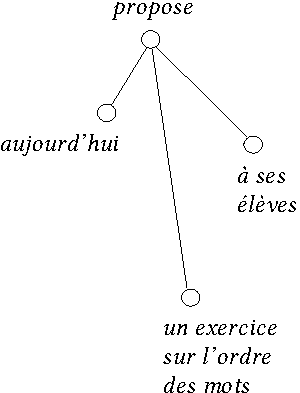
\includegraphics[scale=0.9]{figures/polygraphs/graph-3.5.22.pdf}
\end{figure}

    La position finale d’un dépendant se trouve alors déterminée par la «~longueur~» initiale de la dépendance (déterminée par la fonction et la nature du dépendant comme dans le modèle avec gabarit), l’\hi{élasticité} de cette dépendance et différents paramètres comme le poids ou la saillance.
}
\globe[sec:3.5.23]{Les langues dites à ordre libre}{%
    Une langue est dite \textstyleTermesapprof{à ordre libre} quand une tête et ses dépendants (et notamment le verbe, son sujet et son objet) peuvent être dans n’importe quel ordre. Lorsque, au contraire, un seul ordre est possible, on dit que la langue est \textstyleTermesapprof{à ordre rigide}. Il existe entre les deux toute une gamme de langues à ordre plus ou moins libre ou plus ou moins rigide.

    L’ordre des mots en français est particulièrement rigide, même s’il l’est un peu moins qu’en anglais. L’allemand a un ordre plus libre que le français. Par exemple, on peut traduire \textit{Marie poursuit Pierre} par \textit{die Marie verfolgt den Pierre} ou bien par \textit{den Pierre verfolgt die Marie.} Les deux phrases ont le même \hi{contenu informationnel} (voir chapitre \ref{sec:1.2}), c’est-à-dire qu’elles décrivent le même état du monde : chaque fois c’est Marie qui poursuit Pierre et pas l’inverse. Le repérage des dépendants du verbe est effectué en allemand grâce à un \textstyleTermesapprof{système casuel}, c’est-à-dire des marques sur certains mots du syntagme substantival qui n’ont pas d’autre rôle que justement d’indiquer la relation qu’entretient le syntagme avec le verbe. (Voir la notion de \textit{cas} au \chapfuturef{15}.) Ce sont avant tout les déterminants qui portent l’information casuelle en allemand. Dans notre exemple, le fait que \textit{den Pierre} soit l’objet est marqué par le cas accusatif du déterminant masculin singulier \textit{den} (qui s’oppose à la forme nominative \textit{der} de l'article défini).

    L’ordre des mots en allemand n’est cependant pas totalement libre au sens où seuls deux des six ordres possibles entre les trois mots correspondant à \textit{Marie}, \textit{Pierre} et \textit{poursuit} sont possibles pour une phrase déclarative. Il existe d’autres langues, comme les langues slaves ou le grec moderne, où les six ordres des trois mots sont acceptables et désignent le même état du monde. Voici un exemple du russe :
    
\ea\label{ex:malinu}
    \ea\itshape    Vanya prigotovil malinu\\
    \glt  ‘Vanya a préparé les framboises’ \\
    \glt  ‘Ce que Vanya a préparé, c’est les framboises’

    \ex\itshape Prigotovil Vanya malinu
    \glt ‘Ce qu’a préparé Vanya, c’est les framboises’

    \ex\itshape Malinu prigotovil Vanya
    \glt  ‘C’est les framboises qu’a préparé Vanya’

    \ex\itshape Malinu Vanya prigotovil
    \glt   ‘C’est les framboises que Vanya a préparé’

    \ex\itshape Prigotovil malinu Vanya
    \glt ‘Ce qu’il a préparé, c’est les framboises, Vanya’

    \ex\itshape Vanya malinu prigotovil
    \glt  ‘Vanya, c’est les framboises qu’il a préparé’
\z
\z
    Nous avons donné ici les traductions en français lorsque ces phrases répondent à une question sous-jacente telle \textit{Qu’a préparé Vanya} ?, c’est-à-dire que \textit{malinu} ‘les framboises’ est le \textstyleTermesapprof{rhème} (ce qu’on dit), tandis que \textit{Vanya prigotovil} ‘Vanya a préparé’ est le \textstyleTermesapprof{thème} (ce dont on parle).

    Si on regarde les traductions françaises, on remarque que les variations entre ces phrases sont constituées de constructions qui servent à mettre en avant un élément de la phrase. La construction clivée en «~\textit{C’est … que}~», appelée \textstyleTermesapprof{clivée} (voir le test de clivage dans la \sectref{sec:3.4.9}) est utilisée dans les traductions des phrases (\ref{ex:malinu}c, d et f) pour mettre en valeur un élément rhématique non verbal~(ici \textit{les framboises}). Très similaire est la construction pseudo-clivée en «~Ce que …, c’est … » utilisée pour les traductions des phrases (\ref{ex:malinu}a, b et e). À ces constructions s’opposent la \textstyleTermesapprof{dislocation gauche}, qui sert à distinguer un élément thématique, comme \textit{Vanya} dans la traduction de la phrase (\ref{ex:malinu}f). Similairement, on peut aussi disloquer un élément thématique à droite comme \textit{Vanya} dans la traduction de phrase (\ref{ex:malinu}e). Les six ordres en russe s’accompagnent évidemment de légères différences de sens, relevant de la structure communicative (voir l’encadré suivant), similaires à celles que montrent leurs traductions en français. Il n’en reste pas moins que les six ordres sont possibles.

    Notez ensuite que, abstraction faite des mots fonctionnels des différentes constructions, dans les deux langues considérées, le russe et le français, les trois mots lexicaux se trouvent toujours dans le même ordre. À cela s’ajoute que les principaux prosodèmes, qui constituent l’intonation de la phrase se ressemblent pour chacun des ordres possibles. La phrase (\ref{ex:malinu}b) par exemple, a une courbe intonative que l’on peut schématiser comme suit, avec une intonation montante sur le thème (\textit{prigotovil Vanya}) et une intonation descendante sur le rhème (\textit{malinu}).

    \ea
    \attop{%
    \begin{tikzpicture}
    \matrix (matrix) [matrix of nodes, nodes in empty cells, column sep=3mm, row sep=-8pt,
                      ampersand replacement=\&,every node/.style={font=\strut,anchor=base west}]
      {
        \phantom{Vrigotovil} \& \phantom{Vanya}\&  \vphantom{V}\hphantom{alinu}\\
        \textit{Prigotovil}  \& \textit{Vanya} \&  \textit{malinu}\\
        ‘Ce que prépare      \&   Vanya,       \& c’est les framboises’\\
      }; 
      \draw (matrix-1-1.west) -- (matrix-1-2.center) -- (matrix-1-2.north east);
      \draw (matrix-1-3.north west) -- (matrix-1-3.north) -- (matrix-1-3.east);
    \end{tikzpicture}}
    \z

    Il paraît évident qu’il existe une relation entre l’existence d’un système casuel et la liberté dans le placement des arguments verbaux : il serait en effet redondant d’obliger un objet à la fois à porter un marqueur casuel d’accusatif \textit{et} à occuper une place fixe. L’inverse, par contre, n’est pas tout à fait vrai. Une langue sans système casuel n’est pas forcément très restrictive quant à l’ordre des arguments verbaux. Un bel exemple est l'indonésien (et sa variante dialectale, le malais), qui ne connaît pas de flexion casuelle et permet pourtant une plus grande liberté de mots que d’autres langues sans flexion. Si l’ordre dominant est l’ordre SVO comme dans la phrase (\ref{ex:bahasa}a), il est possible de postposer le sujet comme en b et d’antéposer l’objet comme en c.
    
    \ea\label{ex:bahasa}
    \ea
    \gll Ali baca buku itu.\\
    Ali lire    livre  ce\\
    \glt  ‘Ali lit ce livre’
    \ex
    \gll baca buku itu Ali.\\
    lire    livre  ce Ali\\
    \glt  ‘Il lit ce livre, Ali’
    \ex
    \gll buku itu Ali baca.\\
        livre ce Ali lire    \\
    \glt  ‘Ce livre, Ali le lit’
    \z
    \z

    On peut comparer cette situation avec celle que propose le français à l’oral, où, avec les dislocations gauches et droites, les six ordres sont possibles sans qu’il n’y ait aucune marque casuelle indiquant les rôles syntaxiques de \textit{Ali} et \textit{ce livre} :

    \ea
    \ea\itshape {Ali, ce livre, il le lit.}
    \ex\itshape {Ali, il le lit, ce livre.}
    \ex\itshape {Il le lit, Ali, ce livre.}
    \ex\itshape {Ce livre, Ali, il le lit.}
    \ex\itshape {Ce livre, il le lit, Ali.}
    \ex\itshape {Il le lit, ce livre, Ali.}
    \z
    \z
C'est la sémantique de \textsc{lire} et le caractère animé de \textit{Ali} et non animé de \textit{ce livre} qui permit de savoir qui est sujet ou objet du verbe.
}
\globe[sec:3.5.24]{Ordre communicativement dirigé}{%
    Les \hi{langues à ordre rigide} (voir l’encadré qui précède) sont généralement des langues où la position topologique est fortement déterminée par la fonction syntaxique et la catégorie syntaxique. Ainsi, en français, un objet direct doit nécessairement être après le verbe, à moins que ce soit un clitique, un pronom relatif ou un pronom interrogatif. Autrement dit, en français, l’ordre linéaire est utilisé pour marquer la fonction syntaxique et permettre le repérage de l’objet par rapport au sujet. Nous dirons que de telles langues ont un \textstyleTermesapprof{ordre syntaxiquement dirigé}.

    A l’inverse dans \hi{les langues à ordre libre}, la fonction syntaxique joue peu de rôle, puisque, quelle que soit la fonction syntaxique, tous les ordres sont possibles. Il ne faut pas croire pour autant que l’ordre dans ces langues soit non motivé et que tous les ordres se valent. Il existe un \hi{principe d’économie} qui veut que les langues cherchent à en dire le maximum avec le minimum de moyens : il n’est donc même pas imaginable qu’un moyen aussi disponible que l’ordre linéaire ne soit pas exploitée par la grammaire. À quelle fin est alors utilisé l’ordre linéaire quand il ne sert pas à exprimer la fonction syntaxique ?

    Il semble que, dès que l’ordre n’est pas syntaxiquement dirigé, il serve principalement à exprimer la \textstyleTermesapprof{structure communicative} (voir l’\encadref{sec:1.2.4} sur \textit{Les composantes du sens}) et en particulier à indiquer de quoi on parle et ce qu’on en dit (l’\textstyleTermesapprof{opposition thème/rhème}) et ce que l’on souhaite contraster (la \textstyleTermesapprof{focalisation}). Les langues à ordre libre sont donc généralement des langues à \textstyleTermesapprof{ordre communicativement dirigé}.

    Nous avons vu, dans l’encadré qui précède, que le russe permettait tous les ordres possibles du verbe avec son sujet et son objet. Les traductions que nous avons proposées montrent que ces variations d’ordres correspondent en français à des constructions telles que le clivage ou la dislocation. En français, le clivage sert à marquer un \hi{rhème focalisé~}: autrement dit, dans la phrase \textbf{\textit{C’est}} \textit{les framboises} \textbf{\textit{que}} \textit{Vanya préfère}, non seulement \textit{les framboises} est rhématique (ce qu’on dit, l’information qui est communiquée, c’est \textit{les framboises}), mais en plus cette information est \textstyleTermesapprof{focalisée}, c’est-à-dire qu’elle est contrastée avec tous les autres éléments qui pourraient occuper cette position : c’est les framboises qu’il préfère, à l’exclusion de toutes les autres choses pertinentes dans le contexte d’énonciation. La dislocation gauche quant à elle sert à marquer un \hi{thème focalisé~}: autrement dit, dans la phrase \textit{Les framboises, Vanya aime ça}, non seulement \textit{les framboises} est thématique (ce dont on parle, ce qui est le thème de l’information que je vais communiquer, c’est \textit{les framboises}), mais en plus cette information est focalisée, c’est-à-dire qu’elle est contrastée avec tous les autres éléments qui pourraient occuper cette position dans le contexte d’énonciation : les framboises, il aime ça, les autres fruits rouges, c’est moins sûr.

    On peut postuler qu’en russe, l’ordre linéaire de la phrase obéit au gabarit de la figure \ref{fig:topo-russe}.

    \begin{figure}[H]
    \caption{Gabarit topologique de la phrase en russe\label{fig:topo-russe}}
    \begin{tabular}{|c|c|c|}
     \hline
    \multicolumn{3}{|c|}{\cellcolor{lsDOIGray}Domaine principal}\\
    \hhline{---}
    thème-foc & rhème & thème\\
    \hhline{---}
    \end{tabular}
    \end{figure}

    Le verbe en fonction de sa valeur communicative va venir dans un des trois champs. Les dépendants qui on la même valeur communicative que lui se placeront dans le même champ, tandis que ceux qui ont d’autres valeurs iront dans d’autres champs. La prosodie viendra souligner cette répartition avec une intonation montante sur le thème focalisé, descendante sur le rhème et généralement plate sur le thème.

    C’est à Henri Weil, dans sa thèse publiée en \citeyear{weil1844de} (déjà mentionné dans l’\encadref{sec:3.5.12} sur les \textit{Langues à têtes finales et langues à têtes initiales}), que l’on doit d’avoir introduit les notions de thème et rhème et d’avoir noté que trois facteurs pouvaient influencer l’ordre des mots : la structure de dépendance, la structure communicative et la prosodie. En comparant le français, l’anglais, l’allemand, le turc, le chinois, le latin et le grec ancien, il remarque que certaines langues ont un ordre davantage contrôlé par la syntaxe (les langues dites à ordre rigide) et d’autres davantage contrôlé par la structure communicative (les langues dites à ordre libre).
}

\loupe[sec:3.5.25]{Les autres usages de l’ordre linéaire}{%
    Nous venons de voir, dans les deux encadrés qui précèdent, les deux principaux usages de l’ordre linéaire : le marquage de la fonction syntaxique et le marquage de la structure communicative. Il existe trois autres usages de l’ordre linéaire.

    Premièrement, certains syntaxèmes peuvent avoir des contraintes de placement très particulières. En arabe, par exemple, le déterminant défini se place devant le nom (\textit{\textbf{al}-}ʔ\textit{awlaad-u}, \textsc{def}-enfant-\textsc{nom.pl} ‘les enfants’), alors que l’indéfini se place après (\textit{ʔawlaad-u-\textbf{n}}, enfant-\textsc{nom.pl-indef} ‘des enfants’). En français, certains adjectifs tendent à se placer devant le verbe (\textit{un} \textbf{\textit{petit}} \textit{ballon}), certains se placent obligatoirement après (\textit{un ballon} \textbf{\textit{rouge}}), tandis que, pour d’autres encore, l’ordre est relativement libre (\textit{un} \textbf{\textit{superbe}} \textit{ballon~}; \textit{un ballon} \textbf{\textit{superbe}}). Certains adjectifs peuvent avoir selon leur acception des placements différents : \textit{un homme grand} (un homme grand parmi les hommes) vs \textit{un grand homme} (un homme grand dans l’humanité), \textit{un marié jeune} (une personne jeune parmi les mariés) vs \textit{un jeune marié} (une personne jeune dans son mariage).

    Deuxièmement, les mêmes éléments lexicaux peuvent selon l’ordre déclencher des constructions différentes. Tel est le cas en russe : le numéral se place normalement devant le nom, comme dans \textit{sto metrov} ‘cent mètres’, mais on peut aussi placer le numéral après le nom. Néanmoins, il s’agit d’une autre construction, car le sens change : \textit{metrov sto} ‘approximativement cent mètres’.

    Troisièmement, les différences d'ordre des mots entraînent des différences de portée et donc de sens : \textit{Le lundi, Pierre travaille à Paris} (chaque lundi Pierre est à Paris) vs. À \textit{Paris, Pierre travaille le lundi} (quand Pierre n’est pas à Paris on ne sait pas ce qu’il fait le lundi). On peut imputer la différence de sens des deux phrases à une différence de structure communicative : dans la première \textit{lundi} est un thème focalisé, alors que c’est \textit{à Paris} dans la deuxième. Néanmoins, la différence de portée entraîne aussi une différence de sens informationnel, puisque les deux phrases peuvent correspondre à des situations du monde différentes.
}
\section{Modèle topologique}\label{sec:3.5.26}

Nous allons voir de manière un peu plus précise comment fonctionne le modèle topologique basé sur les gabarits.

Nous avons donné le gabarit topologique du verbe à l’indicatif en français dans la figure \ref{fig:domaine-verbal}. Nous donnons le gabarit topologique du nom en français dans la figure \ref{fig:domaine-nominal}.
Le nom possède un champ final à sa droite où les compléments peuvent se placer assez librement (avec des préférences en fonction de leur poids et de leur saillance), tandis que l’ordre à gauche du nom est assez rigide : ainsi, un syntagme comme \textit{les deux seules autres petites tables} n’accepte pas d’autre ordre que celui qu’il a. Voir l’\encadref{sec:3.5.27} sur la \textit{Topologie du groupe substantival en français}.

\begin{figure}\small
\caption{Gabarit topologique du domaine nominal\label{fig:domaine-nominal}}
\begin{tabular}{|c|c|c|c|c|c|c|c|c|}
\hline
\multicolumn{9}{|c|}{\cellcolor{lsDOIGray}Domaine nominal}\\
\hline
\rotatebox{90}{ch-tout} &  \rotatebox{90}{ch-article~} &  \rotatebox{90}{ch-num} &  \rotatebox{90}{ch-seul} &  \rotatebox{90}{ch-autre} &  \rotatebox{90}{ch-adj} &  \cellcolor{lsDOIGray}\rotatebox{90}{ch-nom} &  \rotatebox{90}{ch-deN} &  \rotatebox{90}{ch-final}\\
\hline
\end{tabular}
\end{figure}

Voyons maintenant comment linéariser un arbre de dépendance. Nous redonnons dans la figure \ref{fig:ballon-dep2} l'arbre de dépendance discuté dans la \sectref{sec:3.5.19} sur \textit{La linéarisation des codépendants}.

\begin{figure}
\begin{tikzpicture}
    \begin{scope}[every node/.style={CircleNode},level distance=2\baselineskip,
                  level 1/.style={sibling distance=20mm},
                  level 2/.style={sibling distance=15mm},
                  level 3/.style={sibling distance=10mm}
                  ]
      \node (root) {} child { node{} child { node{} } child { node{} } edge from parent node [reset shape,midway,above] {sujet} }
                      child { node{} }
                      child { node [xshift=-7mm] {} }
                      child { node [xshift=-7mm] {} }
                      child { node [xshift=-7mm] {} child { node [xshift=5mm] {} } child { node [xshift=5mm] {} } child { node [xshift=5mm] {} } edge from parent node [reset shape,midway,above] {objet} };
    \end{scope}
    \begin{scope}[every node/.style={font=\itshape\strut}]
    \node [above=1pt of root] {prêtera};
    \node [left=1pt of root-1] {garçon};
    \node [below=1pt of root-1-1] {le};
    \node [below=1pt of root-1-2] {petit};
    \node [below=1pt of root-2] {lui};
    \node [below=1pt of root-3] {ne};
    \node [below=1pt of root-4] {pas};
    \node [right=1pt of root-5] {ballon};
    \node [below=1pt of root-5-1] {son};
    \node [below=1pt of root-5-2] {gros};
    \node [below=1pt of root-5-3] {autre};
    \end{scope}
\end{tikzpicture}
\caption{\label{fig:ballon-dep2}Arbre de dépendance de \REF{ex:ballon}}
\end{figure}

Nous procédons en parcourant l’arbre de dépendance à partir de la racine. On commence donc par considérer le verbe \textit{prêtera} qui va ouvrir un domaine verbal. Les règles d’ordre indiquent pour chaque dépendant dans quel champ il peut aller en fonction de sa nature et de sa fonction : un sujet peut aller dans le champ ch-initial, un clitique dans un champ ch-cl-X, etc. On obtient au final la configuration suivante (où les champs non remplis ne sont pas représentés) :

\ea\hfill \begin{tabular}{|c|c|c|c|c|c|}
\hline
garçon & ne & lui & \cellcolor{lsDOIGray}prêtera & pas & ballon\\
\hline
\end{tabular}
\hfill\hbox{}\z

Chaque mot va ensuite ouvrir dans la position qu’il occupe un constituant topologique qui accueillera ses dépendants. Le gabarit du constituant dépendra de la nature de l’élément qui l’ouvre et du champ qu’il occupe (voir, pour le rôle joué par le champ, le cas des adjectifs du français dans l’\encadref{sec:3.5.27}, et celui des verbes en allemand dans l’\encadref{sec:3.5.36} sur \textit{La structure topologique de l’allemand}). Ainsi les noms \textit{garçon} et \textit{ballon} vont-ils ouvrir des domaines nominaux, pour accueillir leurs dépendants, et donner l’ordre final suivant :

\ea\label{ex:topo-ballon}%
\resizebox{.995\linewidth}{!}{\def\arraystretch{1.5}\begin{tabular}{|l|l|l|l|l|l|}
\hline
& & &\cellcolor{lsDOIGray} & & \\[-18pt]
  {\def\arraystretch{1}
  \begin{tabular}{@{}|l|l|l|@{}}
  \hline
    \rotatebox{0}{le} & \rotatebox{0}{petit} & \cellcolor{lsDOIGray} \rotatebox{0}{garçon}\\
  \hline
  \end{tabular}}
  & \rotatebox{0}{ne} & \rotatebox{0}{lui} & \cellcolor{lsDOIGray} \rotatebox{0}{prêtera} & \rotatebox{0}{pas} &
  {\def\arraystretch{1}
  \begin{tabular}{@{}|l|l|l|l|@{}}
    \hline
    \rotatebox{0}{son} & \rotatebox{0}{autre} & \rotatebox{0}{gros} & \cellcolor{lsDOIGray} \rotatebox{0}{ballon}\\
    \hline
  \end{tabular}}\\[-15pt]
   & & &\cellcolor{lsDOIGray} \raisebox{5.5pt}{prêtera} & & \\
\hline
\end{tabular}}\z

On notera qu’en plus de l’ordre linéaire, nous avons obtenu une structure avec des constituants emboîtés.

\Definition{\textstyleTermes{structure topologique}}{La structure d'\hi{emboîtement} que forme les \hi{constituants topologiques} est appelée la \textstyleTermes{structure topologique}. Dans une structure topologique, chaque constituant occupe un \hi{champ topologique}.}

La structure topologique est un \textstyleTermes{arbre de constituants ordonné}, c’est-à-dire un arbre de constituants  avec un ordre linéaire sur les fils de chaque nœud (voir l’\encadref{sec:3.5.28} sur \textit{Arbre de constituants ordonné}). Dans le cas de la structure topologique, l’ordre linéaire sur les fils d’un nœud est donné par le gabarit du constituant, qui est une liste linéairement ordonnée de champs. Les structures topologiques se distinguent notamment des arbres de constituants syntaxiques par le fait chaque constituant est associé à un champ topologique.

La structure topologique de l'exemple \REF{ex:ballon} est donnée sous la forme d'un emboîtement de constituants en \REF{ex:topo-ballon} et sous forme d'arbre dans la figure \ref{fig:topo-ballon}. La deuxième représentation comporte en plus des étiquettes catégorielles sur les constituants topologiques. Il est encore possible d'enrichir la représentation en ajoutant pour  le nom du champ occupé par chaque constituant.

\begin{figure}
\begin{tikzpicture}
    \begin{scope}[every node/.style={CircleNode},level distance=2\baselineskip,
                  level 1/.style={sibling distance=18mm},
                  level 2/.style={sibling distance=9mm},
                  ]
      \node (root) {} child { node{} child { node{} } child { node{} } child { node{} } } 
                      child { node [xshift = 3mm] {} }
                      child { node [xshift = 1mm] {} }
                      child { node [xshift = -1mm] {} }
                      child { node [xshift = -3mm] {} }
                      child { node{} child { node{} } child { node{} } child { node{} } child { node{} } }; 
    \end{scope}
    \node [above=1pt of root] {domaine verbal};
    \node [above left=1pt of root-1,align=center] {\strut domaine\\nominal};
    \node [above right=1pt of root-6,align=center] {\strut domaine\\nominal};
    \begin{scope}[every node/.style={font=\itshape\strut}]
    \node [below=1pt of root-1-1] {le};
    \node [below=1pt of root-1-2] {petit};
    \node [below=1pt of root-1-3] {garçon};
    \node [below=1pt of root-2] {ne};
    \node [below=1pt of root-3] {lui};
    \node [below=1pt of root-4] {prêtera};
    \node [below=1pt of root-5] {pas};
    \node [below=1pt of root-6-1] {son};
    \node [below=1pt of root-6-2] {autre};
    \node [below=1pt of root-6-3] {gros};
    \node [below=1pt of root-6-4] {ballon};
    \end{scope}
\end{tikzpicture}
\caption{\label{fig:topo-ballon}Arbre topologique}
\end{figure}


\eiffel[sec:3.5.27]{Topologie du groupe substantival en français}{%
    Dans le gabarit pour le nom de la figure \ref{fig:domaine-nominal} figure un champ ch-deN, juste après le champ qu’occupe le nom. Il existe en effet une contrainte d’ordre qui concerne les compléments en \textit{de} N (préposition \textsc{de} suivi d’un \hi{nom nu}, c’est-à-dire sans déterminant). Prenons l’exemple des dépendants possibles du syntagme \textit{une chemise}. Nous pouvons modifier \textit{une chemise} par \textit{pour homme}, \textit{en coton} ou \textit{pour le sport}. Chacun de ces trois compléments peut aussi être réalisé par un complément en \textit{de} N : \textit{d’homme}, \textit{de coton}, \textit{de sport}. 
    Contrairement à leurs équivalents, les compléments en \textit{de} N supportent très mal d’être séparé du nom : alors qu’on dira
    (\ref{ex:coton}a), on dira difficilement b et on préférera c.
     
    \ea\label{ex:coton}\judgewidth{\textsuperscript{??}}
    \ea[]{\textit{une chemise orange en coton}}
    \ex[\textsuperscript{??}]{\textit{une chemise orange de coton}}
   \ex[]{\textit{une chemise de coton orange}}
   \z\z
   
   Il semble également difficile de réaliser deux compléments en \textit{de} N, comme en (\ref{ex:coton2}a). Quand on réalise un complément en \textit{de} N avec un autre complément prépositionnel, le complément en \textit{de} N doit précéder l’autre : (\ref{ex:coton2}b) est préférable à c et d à e.
  
  \ea\label{ex:coton2}\judgewidth{\textsuperscript{??}}
   \ea[\textsuperscript{??}]{\textit{une chemise de coton de sport}}
   \ex[]{\textit{une chemise de coton pour le sport}}
   \ex[\textsuperscript{??}]{\textit{une chemise pour le sport de coton}}
   \ex[]{\textit{une chemise de sport en coton}}
   \ex[\textsuperscript{??}]{\textit{une chemise en coton de sport}}
   \z
  \z

    Pour les autres dépendants postposés au nom (adjectifs, compléments prépositionnels, participiales, relatives), nous considérons qu’ils vont tous dans un même champ, car leur ordre est relativement libre et semble suivre avant tout des contraintes de poids. Ainsi un adjectif se placera-t-il plutôt avant un complément prépositionnel (\textit{un mur ancien en pierre}), mais pour peu que cet adjectif soit un peu plus lourd, il se place sans difficulté après le complément prépositionnel (\textit{un mur en pierre très ancien}).

    L’ordre des éléments antéposés au nom est lui très contraint. De plus, seul des groupes adjectivaux légers peuvent être antéposés :
    on a (\ref{ex:mur}a et b), mais pas c, où \textit{haut de trois mètres} doit obligatoirement être postposé au nom comme en d
    (voir aussi l’\encadref{sec:3.5.22} sur les \textit{Contraintes de poids}). 
    
    \ea\label{ex:mur}
    \ea[]{\textit{un} \textbf{\textit{haut}} \textit{mur}}
    \ex[]{\textit{un} \textbf{\textit{très haut}} \textit{mur}}
    \ex[*]{\textit{un} \textbf{\textit{haut de trois mètres}} \textit{mur}}
   \ex[]{\textit{un mur} \textbf{\textit{haut de trois mètres}}}
    \z
    \z
    
    Du point de vue du modèle topologique, cela signifie que l’adjectif \textit{haut} n’ouvre pas un domaine adjectival complet lorsqu’il est antéposé, mais un \textstyleTermes{domaine réduit} où ne figure pas le champ final qui accueille normalement les compléments de l’adjectif. Voir la figure \ref{fig:domaine-adj} : le domaine adjectival complet est utilisé à droite du verbe comme en (\ref{ex:mur}d), tandis que le domaine réduit sera utilisé à gauche du verbe comme en (\ref{ex:mur}a) et b et bloque c, puisqu'il n'y aura pas de place pour le complément prépositionnel de l'adjectif.
    
    Quant à l’ordre relatif des adjectifs antéposés, évoqué à la \sectref{sec:3.5.26}, il semble aller des \hi{éléments à valeur référentielle} à des \hi{adjectifs qualificatifs}. Ces derniers qualifient le référent, en précisent la nature, tandis que les premiers précisent la nature de la référence elle-même : l’article indique si le référent est connu ou pas, le numéral donne le nombre de référents, des adjectifs comme \textit{seul} ou \textit{autre} permettent de positionner le référent dans l’ensemble des référents potentiels.

\begin{figure}[H]
    \caption{Gabarits pour les domaines adjectivaux}
    \label{fig:domaine-adj}
        \begin{center}
    \def\arraystretch{1.5}
    \setlength{\tabcolsep}{4ex}
    \begin{tabular}{|c|c|c|}
    \hline
    \multicolumn{3}{|c|}{\cellcolor{lsDOIGray}Domaine adjectival}\\\hline
    ch-adv & \cellcolor{lsDOIGray} ch-adjectif & ch-final\\
    \hline
    \end{tabular}
    \end{center}
   \begin{center}
    \def\arraystretch{1.5}
    \setlength{\tabcolsep}{4ex}
    \begin{tabular}{|c|c|}
    \hline
    \multicolumn{2}{|c|}{\cellcolor{lsDOIGray}Domaine adjectival réduit}\\\hline
    ch-adv & \cellcolor{lsDOIGray}ch-adjectif\\
    \hline
    \end{tabular}
    \end{center}
\end{figure}
}
\maths[sec:3.5.28]{Arbre de constituants ordonné}{%
En définissant la structure topologique dans la \sectref{sec:3.5.26} sur le {\textit{Modèle topologique}}, nous avons introduit rapidement la notion d'arbre de constituants ordonné. Nous allons préciser la nature de cette structure et les modes de représentation associés.

    Contrairement au cas des arbres de dépendance ordonnés dont les nœuds sont totalement ordonnés, l’\hi{ordre} sur les nœuds d’un arbre de constituants est \hi{partiel}, puisque deux constituants qui sont dans une relation de partie-tout ne peuvent être dans une relation de précédence l’un par rapport à l’autre et que donc une telle spécification d’ordre ne serait pas pertinente.

L’\hi{ordre linéaire sur les fils de chaque nœud} \hi{interne} de l’arbre induit un unique \hi{ordre linéaire sur les feuilles} de l’arbre. Et réciproquement, l’ordre linéaire sur les feuilles suffit à récupérer l’ordre linéaire sur les fils de chaque nœud interne. La preuve est relativement simple : pour ordonner deux feuilles, il faut rechercher leur premier ancêtre commun, lequel est unique. L’ordre sur les deux feuilles considérées est le même que celui des deux fils de leur ancêtre commun qui se trouvent sur les deux branches qui mènent à elles. Par exemple, pour ordonner \textit{garçon} et \textit{ne} dans l’exemple \REF{ex:ballon}, il faut remonter à leur ancêtre commun qui est le nœud du domaine verbal. On en déduit que \textit{garçon} est avant \textit{ne}, car le domaine nominal est avant \textit{ne}.

    Il est possible en théorie de considérer des arbres de constituants avec n’importe quel ordre sur les feuilles de l’arbre, mais cela peut donner des arbres avec des constituants discontinus et
    nous ne sommes en pratique intéressés que par les arbres de constituants ordonnés dont tous les \hi{constituants} sont \hi{continus} (ce qui est le cas des arbres de constituants topologiques et de la plupart des arbres syntaxiques considérés par les grammaires de constituants). C'est pourquoi nous définissons l'ordre dans les arbres de constituants à partir des fils d'un même nœud.

Nous allons maintenant discuter un point important concernant la représentation des arbres de constituants ordonnés.
On peut voir les «~nœuds~» de l’arbre de constituants ordonné non pas comme de simples nœuds, mais comme des segments ayant un début et une fin. N’oublions pas que les nœuds d’un arbre de constituants sont des constituants d’un énoncé et que les constituants d’un énoncé sont des segments continus de cet énoncé. On peut alors représenter les constituants comme des arcs allant d’un nœud début à un nœud fin.  Lesquels nœuds correspondent en fait aux positions linéaires inter-mot (si les constituants minimaux sont les mots) (voir l'\encadref{sec:3.5.17} sur le \textit{{Flux de dépendances}}, où il en a déjà été question).
Nous allons expliciter ce point en proposant deux représentation du même arbre de constituants ordonné, l'arbre de constituant X-barre usuel de la phrase :

\ea\textit{Le chat poursuit un chien.}\z

La première représentation, donnée dans la figure \ref{fig:arbre-tradi},
est
la \hi{représentation traditionnelle} d'un arbre de constituants ordonné, où
la \hi{structure d'arbre} est \hi{explicite} et
l'\hi{ordre} est \hi{implicite}, c’est-à-dire qu’il est représenté par la \hi{position relative des nœuds sur l’axe horizontal}, mais n’est pas explicitement encodé par des relations de précédence entre nœuds.

Dans la deuxième représentation, donnée dans la figure \ref{fig:arbre-cellule},  l’\hi{ordre} est \hi{explicite} et la \hi{structure d'arbre} est \hi{implicite} et peut se déduire de la \hi{position relative des constituants sur l’axe vertical}. Les nœuds du graphe représentent les \hi{positions inter-mot} et les constituants sont représentés par des arcs qui relient leur début à leur fin.  Bien que cette représentation soit beaucoup moins usuelle, elle est tout aussi simple et légitime que la représentation traditionnelle.  Cette représentation, où chaque décomposition d'un constituant (chaque connexion vue du point de vue dépendentiel) forme une «~cellule~», sera nommée la \hi{représentation en cellules} d'un arbre de constituants ordonné ou plus simplement un \textstyleTermes{arbre de constituants en cellules}.

\begin{figure}[H]
    \caption{Représentation traditionnelle d'un arbre de constituants ordonné (hiérarchie explicite, ordre implicite)\label{fig:arbre-tradi}}
    \begin{forest}
    [\textrm{P}
      [GN [D [\textit{le}]] [N [\textit{chat}]] ]
      [GV [V [\textit{poursuit}]] [GN [D [\textit{un}] ] [N [\textit{chien}] ] ] ]
    ]
    \end{forest}
 \end{figure}

\begin{figure}[H]
    \caption{Représentation en cellules d'un arbre de constituants ordonné (hiérarchie implicite, ordre explicite)\label{fig:arbre-cellule}}
\begin{tikzpicture}
    \begin{scope}[every node/.style={CircleNode},grow=right]
    \node (root) {} child { node {} child { node{} child { node{} child { node{}  
                    child { node{} } } } } }; 
    \end{scope}      
     \path (root)         edge[bend left] node[midway, above] {D} (root-1)
           (root-1)       edge[bend left] node[midway, above] {N} (root-1-1)
           (root-1-1)     edge[bend left] node[midway, above] {V} (root-1-1-1)
           (root-1-1-1)   edge[bend left] node[midway, above] {D} (root-1-1-1-1)
           (root-1-1-1-1) edge[bend left] node[midway, above] {N} (root-1-1-1-1-1)
           (root)         edge[bend left=66] node[midway, above] {GN} (root-1-1)
           (root-1-1-1)   edge[bend left=66] node[midway, above] {GN} (root-1-1-1-1-1)
           (root-1-1)     edge[bend left=90] node[midway, above] {GV} (root-1-1-1-1-1)
           (root)         edge[bend left=90] node[midway, above] {P} (root-1-1-1-1-1);
           
     \coordinate (1) at ($ (root) !.5! (root-1) $);
     \coordinate (2) at ($ (root-1) !.5! (root-1-1) $);
     \coordinate (3) at ($ (root-1-1) !.5! (root-1-1-1) $);
     \coordinate (4) at ($ (root-1-1-1) !.5! (root-1-1-1-1) $);
     \coordinate (5) at ($ (root-1-1-1-1) !.5! (root-1-1-1-1-1) $);
     
    \foreach \pos/\text in {1/le,2/chat,3/poursuit,4/un,5/chien} 
      {\node [font={\itshape\strut}, below=1pt of \pos] {\text};}
\end{tikzpicture}
 \end{figure}

Notons qu'il est possible de combiner les deux représentations et d'expliciter à la fois la structure hiérarchique d'arbre et l'ordre linéaire. 
}
\maths[sec:3.5.29]{Grammaires de réécriture}{%
    L’une des premières modélisations mathématiques de la grammaire est la \textstyleTermesapprof{grammaire de réécriture} proposée par Noam \citet{chomsky1957syntactic} (voir l’\encadref{sec:1.3.7} sur \textit{Calcul symbolique et grammaires catégorielles} pour les toutes premières grammaires formelles). Notre modèle topologique, au travers de ses gabarits, prolonge ce formalisme. Nous commençons par présenter ce formalisme avant d'en expliquer les limites et l'intérêt d'introduire un modèle plus riche comme le modèle topologique.

\tcbsubtitle{Exemple}
    Bien qu’on puisse utiliser les grammaires de réécriture pour définir des grammaires de dépendances, il s’agit au départ d’un formalisme introduit pour écrire des grammaires de constituants. Voici un exemple pour ceux qui ne connaissent pas encore ce formalisme. Les \textstyleTermesapprof{règles} (dites \textstyleTermesapprof{de réécriture}) sont de la forme :

    \ea \label{ex:regles}
    \begin{tabular}[t]{@{}l@{\hspace{4\tabcolsep}}l@{}}
    P → GN GV  &  V → \textit{attrape} {\textbar} \textit{poursuit}\\
    GV → V GN  &  N → \textit{chat} {\textbar} \textit{chien}\\
    GN → D N   & D → \textit{le} {\textbar} \textit{un}\\
    \end{tabular}
    \z

    Avec de telles règles, on peut produire des phrases telles que \textit{le chat poursuit un chien} ou \textit{le chien attrape le chat}. Les règles de droite sont des \textstyleTermesapprof{règles lexicales} (par exemple \textit{attrape} ou \textit{poursuit} sont des constituants de type V). Les règles de gauche sont des \textstyleTermesapprof{règles syntagmatiques} qui disent comment un constituant se décompose. Par exemple, la règle P \textrm{→} GN GV dit qu’une phrase P peut se décomposer en un groupe nominal GN suivi d’un groupe verbal GV. Lue autrement, elle dit comment les constituants se combinent : la combinaison d’un GN suivi d’un GV donne un P. La règle P \textrm{→} GN GV ne dit pas seulement que P se décompose en GN et GV, mais aussi que GN précède GV et que l’extension de P est égale à la somme des extensions de GN et GV.

    On peut réinterpréter les règles syntagmatiques comme des \textstyleTermesapprof{structures élémentaires}, c’est-à-dire des portions de la structure finale, un arbre de constituants ordonné dans notre cas, qui, assemblées, permettent de reconstituer la structure finale. La figure \ref{} donne un exemple pour la règle de réécriture P → GN GV. Nous utilisons les deux modes de représentation d’un arbre de constituants ordonné présentés dans l’encadré précédent.

\begin{figure}[H]
% %     \includegraphics{}
    \caption{La règle de réécriture P → GN GV vue comme une structure élémentaire}
    \label{fig:structureGNGV}
    \begin{subfigure}[c]{.5\linewidth}\centering
        \begin{forest} 
        [P [GN] [GV]]
        \end{forest}
        \caption{Représentation en arbre}
        \end{subfigure}\begin{subfigure}[c]{.5\linewidth}\centering
        \begin{tikzpicture} 
       \node at (0,0) (GN) [CircleNode] {};
       \node at (1,-.75) (empty) [CircleNode] {};
       \node at (2,0) (GV) [CircleNode] {};
%        \node [below=1pt of 1] {P};
%        \node [below left = 2pt of GN] {GN};
%        \node [below right = 2pt of GV] {GV};
       \path (GN) edge [out=270,in=180] node [left,midway] {GN} (empty)
             (empty) edge [out=0,in=270] node [right,midway] {GV} (GV)
             (GN) edge [bend left=66] node [below,midway] {P} (GV);
       \end{tikzpicture}
       \caption{Représentation en cellules}
    \end{subfigure}
 \end{figure}

    Avec les règles proposées en \REF{ex:regles}, et en les considérant comme des structures élémentaires qu'on assemble, on peut générer l’arbre de constituants de la phrase \textit{Le chat poursuit un chien} donné dans l’encadré qui précède. Chaque portion élémentaire de l’arbre, composée d’un nœud et de ses fils, correspond exactement à une règle de réécriture. Ainsi le sommet de l’arbre avec le nœud P et ses deux fils GN et GV est validé par la règle P \textrm{→} GN GV.

  \tcbsubtitle{Critiques}
    Nous souhaitons faire trois critiques concernant une grammaire de constituants comme celle qui précède (qui sert toujours de base à de nombreux modèles linguistiques).

    Passons rapidement sur la première, puisqu’elle a déjà fait abondamment l’objet de ce livre : nous pensons qu’il est plus judicieux de penser la syntaxe d’une langue en termes de connexions et de dépendances qu’en termes de constituants (voir le \chapref{sec:3.2} sur la connexion où nous discutons les problèmes que cela pose de vouloir privilégier une fragmentation parmi toutes celles possibles), bien que, comme nous l’avons montré (\chapref{sec:3.4}), les deux approches sont en grande partie équivalentes.

    La deuxième critique concerne le fait de vouloir \hi{exprimer simultanément la sous-catégorisation} (le fait qu’une phrase P peut être décomposée en un GN et un GV) \hi{et l’ordre linéaire} (le fait que GN < GV). Ceci peut encore se comprendre pour des langues à ordre rigide comme l’anglais, mais est difficilement justifiable pour des langues à ordre libre, où l’ordre linéaire dépend peu des relations syntaxiques (voir l’\encadref{sec:3.5.24} sur \textit{Ordre communicativement dirigé}). Cette critique a été faite dès les années 1970 et les modèles qui ont émergé au début des années 1980, notamment GPSG (\textit{Generalized Phrase Structure Grammar}), la grammaire syntagmatique généralisée de Gerald Gazdar, bien que toujours basée sur une grammaire de réécriture, séparaient clairement les \textstyleTermesapprof{règles }dites\textstyleTermesapprof{ de dominance immédiate} des \textstyleTermesapprof{règles de précédence linéaire} entre constituants.

    La troisième critique permet de saisir une différence essentielle entre les \hi{grammaires} dites \hi{syntagmatiques} (\textit{Phrase Structure Grammars} ou PSG) et les grammaires topologiques. Les règles de précédence linéaire des PSG sont des règles de précédence entre constituants, comme par exemple GN < GV. Or le sujet du verbe n’est pas nécessairement un groupe nominal (\textbf{\textit{Qu’il} \textit{vienne}} \textit{me surprendrait ;} \textbf{\textit{Partir maintenant}} \textit{serait plus judicieux)}. Il faut donc distinguer la catégorie et la fonction. On peut remplacer cette règle par Sujet < V. C’est déjà mieux, mais les grammaires topologiques vont encore plus loin. Comme nous l’avons déjà souligné, en français, le sujet n’est pas toujours devant le verbe, mais pour qu’il n’en soit pas ainsi il faut qu’un autre élément vienne occuper sa place. Il ne faut donc pas seulement \hi{déconnecter} la catégorie de la fonction, mais aussi déconnecter la \hi{fonction} de la position linéaire (c'est-à-dire du \hi{champ} dans notre modélisation). Une grammaire topologique décompose la règle Sujet < V en deux règles : 1) il existe un champ préverbal qui doit être rempli par un et un seul élément et 2) le sujet peut occuper le champ préverbal. (Le fait que le sujet occupe occupe généralement le champ préverbal n'est pas dit dans la règle : cela découle du fait que les règles qui placent le sujet dans un autre champ sont très contraintes et donc rarement déclenchées.)
}
\section{Projection topologique et émancipation}\label{sec:3.5.30}\largerpage

Comme nous venons de le voir, le modèle topologique, en plus d’assurer la linéarisation de l’arbre de dépendance, lui associe un arbre de constituants ordonné, la structure topologique. En cas de \hi{linéarisation projective}, cet arbre est en fait l’\hi{arbre de constituants syntaxiques plat} obtenu à partir des projections maximales des nœuds de l’arbre de dépendance (voir la \sectref{sec:3.4.4} sur \textit{Arbre de constituants plat}).

Nous allons maintenant nous intéresser à la \hi{linéarisation non projective}. Dans ce cas, certaines projections maximales ne sont pas continues. Nous allons voir comment associer un arbre de constituants ordonné avec des constituants continus à un arbre de dépendance, qu’il soit projectif ou non.

\Definition{\textstyleTermes{projection topologique}}
{Pour chaque nœud \textit{x} d’un arbre de dépendance ordonné, nous définissons la \textstyleTermes{projection topologique} de \textit{x} comme le plus grand \hi{segment continu} contenant \textit{x} qui corresponde à une portion connexe de l’arbre de dépendance ayant \textit{x} pour racine.}

Lorsque l’arbre de dépendance est projectif, la projection maximale de chaque nœud est continu et donc la projection topologique d’un nœud est sa projection maximale. Mais, dès qu’un arbre de dépendance est non projectif, la projection topologique de certains nœuds n’est plus leur projection maximale. Reprenons l’exemple \REF{ex:belle-complet} de la \sectref{sec:3.5.14} :

\ea\label{ex:belle}
    \textit{{Une belle est entrée qui voulait les acheter}.}
\z
La projection topologique de \textit{une belle} est \textit{une belle}, alors que sa projection maximale est \textit{une belle qui voulait les acheter}. Par contre, la projection topologique de \textit{est entrée} est bien la phrase entière et donc la projection maximale de \textit{est entrée}.

Les projections topologiques associées à un arbre de dépendance ordonné don\-né forment un arbre de constituants ordonné. Nous appelons cet arbre l’\textstyleTermes{arbre topologique} induit par l’arbre de dépendance ordonné. Il s'agit en général de l'arbre sous-jacent à la structure topologique (qui contient en plus des étiquettes sur la nature des constituants et les champs qu'ils occupent, voir la \sectref{sec:3.5.26} sur le {\textit{Modèle topologique}}). Nous verrons dans l'\encadref{sec:3.5.A} un cas d'\textit{Émanci\-pa\-tion projective}, où l'arbre topologique ne correspond pas à la structure topologique. Par ailleurs, la structure topologique peut être plus riche que l'arbre topologique induit dès que l'on considère des constituants topologiques intermédiaires (voir la \sectref{sec:3.5.34} éponyme).

Nous donnons, dans la figure \ref{fig:induit-topo}, l'arbre topologique à partir d'un arbre de dépendance à gros grains de l'exemple \REF{ex:belle}. Notons qu'il s'agit d'un arbre de constituants avec tête, puisque chaque constituant topologique est la projection d'une tête. Nous explicitons dans la représentation de cet arbre l'ordre linéaire entre les feuilles afin de bien spécifier qu'il s'agit d'un arbre de constituants ordonné, à ne pas confondre avec un arbre de constituants syntaxiques, comme introduit au \chapref{sec:3.4} et qui n'est pas ordonné.

\begin{figure}
\begin{minipage}[c]{.45\linewidth}\centering
\begin{tikzpicture}[>={Triangle[]}]
  \begin{scope}[every node/.style={CircleNode},grow=right,level distance=2cm]
  \node at (0,0) (root) {} child { node {} child { node{} } };
  \path (root) edge [bend left=45,->] (root-1-1)
        (root-1) edge [bend right,->] (root);
  \end{scope}
  \draw [<-] (root-1) -- ++(0,1.5cm);
  \node [below=1pt of root, font=\itshape\strut] {une belle};
  \node [below=1pt of root-1, font=\itshape\strut] {est entrée};
  \node [below=1pt of root-1-1, font=\itshape,align=center] {\strut qui voulait\\les acheter};
\end{tikzpicture}
\end{minipage}\begin{minipage}[c]{.1\linewidth}\centering
\huge$\Rightarrow$
\end{minipage}\begin{minipage}[c]{.45\linewidth}\centering
\begin{tikzpicture}
  \begin{scope}[every node/.style={CircleNode},sibling distance=20mm]
  \node (root) {} 
    child { node{} } 
    child { node{} edge from parent node [reset shape, midway, right] {T} } 
    child { node{} };
  \draw (root-1) -- (root-2) -- (root-3);
  \end{scope}
  \node [below=1pt of root-1, font=\itshape\strut] {une belle};
  \node [below=1pt of root-2, font=\itshape\strut] {est entrée};
  \node [below=1pt of root-3, font=\itshape,align=center] {\strut qui voulait\\les acheter};
\end{tikzpicture}
\end{minipage}
\caption{\label{fig:induit-topo}Arbre de dépendance ordonné et arbre de constituants topologiques induit}
\end{figure}

Un arbre de dépendance ordonné induit donc deux arbres de constituants avec têtes : un arbre de constituants syntaxiques et un arbre de constituants topologiques. Nous donnons, dans la figure \ref{fig:induit-synt}, l'arbre de constituants syntaxiques de notre exemple.\largerpage


\begin{figure}
\begin{minipage}[c]{.45\linewidth}\centering
\begin{tikzpicture}[every node/.style={font=\strut\itshape}]
\begin{scope}[
    every node/.style={CircleNode}
    ]
\node (root) {}
    child { node { } 
          child { node { } }
           };
\end{scope}
\node[left=1pt of root] {est entrée};
\node[left=1pt of root-1] {une belle};
\node[left=1pt of root-1-1, align=center] {qui voulait\\les acheter};
\end{tikzpicture}\end{minipage}\begin{minipage}[c]{.1\linewidth} \huge$\Rightarrow$ \end{minipage}%
\begin{minipage}[c]{.45\linewidth}\centering
\begin{tikzpicture}[every node/.style={font=\strut}]
    \begin{scope}[
    every node/.style={CircleNode},
    sibling distance=20mm,
    level distance=3\baselineskip
    ]
        \node (root) {}
            child { node { } child { node { } edge from parent node [reset shape, midway, anchor=base east] {T} } 
                            child { node { } } 
                edge from parent node [reset shape, midway, anchor=base east] {T} }
            child { node { } };
    \end{scope}
    \begin{scope}[every node/.style={font=\strut\itshape}]
    \foreach \pos/\text in {1-1/une belle, 1-2/\strut qui voulait\\les acheter, 2/est entrée} 
      {\node [below=1pt of root-\pos,align=center] {\text};}
    \end{scope}
    \end{tikzpicture}
\end{minipage}
\caption{\label{fig:induit-synt}Arbre de dépendance et arbre de constituants syntaxiques induit}
\end{figure}

La comparaison entre l’arbre topologique induit et l’arbre de constituants syntaxiques nous amène à introduire de nouveaux concepts. 
Comme on le voit dans les figures \ref{fig:induit-topo} et \ref{fig:induit-synt}, la relative \textit{qui voulait les acheter} n’est pas à la même position dans les deux arbres : dans l’arbre syntaxique, la relative est un nœud fils du groupe substantival dont \textit{une belle} est la tête, alors que dans l’arbre topologique, elle est un nœud fils de la phrase entière dont \textit{est entrée} est la tête. Autrement dit, la relative ne s’est pas positionnée par rapport à son gouverneur syntaxique \textit{une belle}, mais par rapport au gouverneur de celui-ci, \textit{est entrée}. Elle n'est pas dans la projection topologique de son gouverneur syntaxique, mais dans celle d'un ancêtre plus lointain.

\Definition{\textstyleTermes{élément émancipé}, \textstyleTermes{hôte topologique}, \textstyleTermes{visiteur topologique}}
{Un nœud de l'arbre de dépendance qui n'est pas dans la projection topologique de son gouverneur syntaxique est dit \textstyleTermes{émancipé}. Son plus proche ancêtre à la projection syntaxique duquel il appartient est son \textstyleTermes{hôte topologique}. Si l’on prend maintenant le point de vue de l’hôte topologique, nous dirons qu’un élément qui vient se placer dans la projection topologique d'un nœud sans en être un dépendant syntaxique est un \textstyleTermes{visiteur topologique}.}

Dans notre exemple, la relative \textit{qui voulait les acheter} est un élément émancipé. Elle est un visiteur topologique de la forme verbale \textit{est entrée}, qui est en retour son hôte topologique.

Un élément émancipé ne se place pas par rapport à son gouverneur, mais par rapport à un ancêtre plus éloigné, son hôte topologique. 
En conséquence, la dépendance qui unit un élément émancipé à son gouverneur syntaxique est nécessairement \hi{non projective} (voir l’\encadref{sec:3.5.16} sur l’\textit{Équivalence des définitions de la projectivité}).


\section{Non-projectivité en français}\label{sec:3.5.32}

Nous allons présenter les principaux cas de non-projectivité en français et voir comment les modéliser.

\subsection{Montée des clitiques}
Considérons les exemples suivants :

\ea
\ea \itshape Zoé \textbf{lui} a parlé.
\ex \itshape Zoé \textbf{y}   est sensible.
\ex \itshape Zoé \textbf{le}  fait appeler par un ami.
\ex \itshape Zoé \textbf{en}  a envie.
\ex \itshape Zoé \textbf{en}  connaît la moitié.
\z
\z

Dans tous ces exemples, le clitique se place sur le verbe fini (son hôte topologique), alors qu’il est régi par un dépendant de ce verbe, qui peut être un participe dans une forme verbale complexe (\textit{a parlé}), un adjectif dans une construction copulative (\textit{est sensible}), un infinitif dans une construction causative (\textit{fait appeler}), un nom prédicatif dans une construction à verbe support (\textit{a envie}) ou même un objet direct dans une construction transitive (\textit{connaît la moitié}).

Autrement dit, le gouverneur syntaxique du clitique n’offre pas de place au clitique, forçant son émancipation. Un participe passé, par exemple, ne peut jamais accueillir des clitiques, qu’il dépende d’un verbe, comme précédemment, ou qu’il dépende d’un nom (\textit{le livre donné à Zoé} vs \textit{*le livre lui donné}). Il va donc ouvrir un constituant avec un gabarit différent de celui d’un verbe fini.
Le domaine verbal réduit est présenté dans la figure \ref{fig:gabarit-verbal-reduit}.

\begin{figure}
\caption{\label{fig:gabarit-verbal-reduit}Gabarit topologique du domaine verbal réduit}
\def\arraystretch{1.5}
\setlength{\tabcolsep}{3ex}
\begin{tabular}{|c|c|c|c|c|}
\hline
\multicolumn{5}{|c|}{\cellcolor{lsDOIGray}Domaine verbal réduit}\\
\hline
ch-adv & \cellcolor{lsDOIGray}ch-verbe & ch-adv & ch-vb-sub & ch-final\\
\hline
\end{tabular}
\end{figure}

Un infinitif peut normalement accueillir des clitiques (\textit{Zoé veut} \textbf{\textit{l’}}\textit{appeler}), mais pas quand il est dans la construction causative (\textit{Zoé le fait appeler} vs *\textit{Zoé fait l'appeler}). Il ouvrira dans ce cas un constituant réduit comme celui d’un participe passé.

\subsection{Comparatif et superlatif}
\begin{sloppypar}
Les constructions comparatives et superlatives des adjectifs en français peuvent être illustrées par :
\end{sloppypar}

\ea\label{ex:plus}
\ea \itshape un plus beau livre \textbf{que le mien}
\ex \itshape le plus beau livre \textbf{du monde}.
\z
\z

Dans ces constructions, le complément à droite du nom dépend de \textit{plus} comme le montre le changement complet de sens lorsque celui-ci est supprimé (\textsuperscript{\#}\textit{un beau livre que le mien} ; \textsuperscript{\#}\textit{le beau livre du monde}), ainsi que la possibilité de le séparer du nom (\textit{ce livre est plus beau que le mien~}; \textit{le livre le plus beau du monde}).

\begin{figure}
\begin{tikzpicture}
\begin{scope}[every node/.style={CircleNode},grow=right]
\node (root) {} child { node {} child { node{} child { node{} child { node{}  
                    child { node{} child { node{} } } } } } }; 
\end{scope}
\foreach \pos/\text in {/un, -1/plus, -1-1/beau, -1-1-1/livre, -1-1-1-1/que,
                        -1-1-1-1-1/le, -1-1-1-1-1-1/mien,} 
      {\node [font={\itshape\strut}, below=1pt of root\pos] {\text};}
      
\path (root-1-1)   edge[bend right,-{Triangle[]}] (root-1)
      (root-1-1-1) edge[bend right,-{Triangle[]}] (root-1-1)
      (root-1-1-1-1-1-1) edge[bend right,-{Triangle[]}] (root-1-1-1-1-1)
      (root-1) edge[bend left,-{Triangle[]},out=60,in=120] (root-1-1-1-1)
      (root-1-1-1-1) edge[bend left,-{Triangle[]},out=60,in=120] (root-1-1-1-1-1-1)
      (root-1-1-1) edge [bend right,-{Triangle[]},out=315,in=225] (root);

\draw[{Triangle[]}-] (root-1-1-1) -- ++(0,2cm);
\end{tikzpicture}
\caption{\label{fig:plus}Arbre de dépendance ordonné de (\ref{ex:plus}a)}
\end{figure}

Le complément du superlatif va donc s’émanciper, non seulement du constituant ouvert par son gouverneur \textit{plus}, mais aussi du constituant ouvert par le gouverneur de celui-ci, \textit{beau,} (c’est-à-dire d’un domaine adjectival réduit, voir l’\encadref{sec:3.5.28} sur la \textit{Topologie du groupe substantival en français}) et venir ainsi se placer dans le champ final du domaine nominal. Ceci est à contraster avec les compléments de l’adjectif, qui ne peuvent s’émanciper de la même façon (\textit{un livre beau à pleurer} vs. *\textit{un beau livre à pleurer}).

\subsection{Extraction}
Donnons quelques exemples de phénomènes dit d'\hi{extraction} :

\ea\label{ex:extraction1}
\ea \itshape \textbf{L’année  prochaine},  je pense que Zoé habitera ailleurs.
\ex \itshape \textbf{A quel endroit}  Zoé a-t-elle envie d’habiter ?
\ex \itshape l’endroit \textbf{où}  il est probable que Zoé habitera.
\z
\z
Dans ces exemples, un complément est placé en tête de la proposition principale : un tel complément est dit extrait. La non-projectivité de ces exemples vient du fait que le gouverneur du complément extrait n'est pas le verbe principal, mais un verbe subordonné (\textit{habiter/habitera}).

Nous consacrerons l’entièreté du \chapfuturef{19}  à l’étude des phénomènes d'extraction, notamment lorsqu’ils mettent en jeu des pronoms interrogatifs ou relatifs. L'exemple (\ref{ex:extraction1}a), qui illustre la \textstyleTermes{topicalisation} d’un complément circonstanciel, peut déjà être modélisé avec les outils introduits dans ce chapitre : il s’agit d’une émancipation du complément \textit{l'année prochaine} qui vient se placer dans le champ pré-noyau ouvert par un verbe à l’indicatif.\largerpage

\loupe{Émancipation projective}
{\label{sec:3.5.A}
Il existe certains cas où, bien que la structure soit projective, on est amené à supposer une émancipation. Nous appelons de tels cas une \textstyleTermes{émancipation projective}. L'émancipation projective est illustrée par des exemples comme (\ref{ex:en}b) ou d, où le complément de nom \textit{de ce film} a été pronominalisé par le pronom relatif \textit{dont} ou le pronom personnel \textit{en}.

\pagebreak\ea\label{ex:en}
\ea \textit{La fin \textbf{de ce film} est particulièrement triste.}
\ex \textit{un film \textbf{dont} la fin est particulièrement triste}
\ex \textit{un film \textbf{dont} il parait que la fin est particulièrement triste}
\ex \textit{La fin \textbf{en} est particulièrement triste.}
\ex \textit{La fin m'\textbf{en} a ému.}
\ex \textit{La fin semble \textbf{en} être particulièrement triste.}
\z\z

Le fait que ces pronoms se substituent au complément du nom \textit{fin} permet de faire l'hypothèse qu'ils dépendent syntaxiquement de ce nom, bien qu'ils ne forment pas avec lui une unité autonomisable (\textit{la fin en} ou \textit{dont la fin} ne sont pas des unités acceptables). Les exemples (\ref{ex:en}c, e et f), qui sont non projectifs, montrent que ces pronoms ne se placent pas par rapport au nom \textit{fin}. Et donc qu'ils s'émancipent pour venir se placer dans un champ ouvert par le verbe. (Le cas de \textit{dont} et des pronoms relatifs sera discuté plus en détail dans le \chapfuturef{19} sur l'\textit{Extraction}.)

Un autre cas d'émancipation projective est illustré par notre analyse de l'ordre des mots en allemand proposé dans l'\encadref{sec:3.5.36} sur \textit{La structure topologique de l’allemand}. Nous considérons que tous les dépendants non verbaux des verbes qui se trouvent dans la parenthèse droite sont émancipés, même si ceux-ci ne créent pas de dépendance non projective. C'est par exemple le cas \textit{in seiner Nase} 'dans son nez' qui est à coté de son gouverneur \textit{zu popeln} 'creuser' dans l'exemple \REF{ex:leider}.
}

\maths[sec:3.5.33]{Grammaire topologique formelle}{%
    On peut donner une version plus formelle de la grammaire topologique, à l’image des grammaires de réécriture (voir l'\encadref{sec:3.5.29} sur la \textit{Grammaire de réécriture}). Une \textstyleTermes{grammaire topologique} assure la correspondance entre un arbre de dépendance et un ordre linéaire et elle construit une structure de constituants en même temps qu’elle assure cette correspondance. Nous allons présenter la grammaire topologique dans le sens de la linéarisation, c’est-à-dire comme le passage d’un arbre de dépendance (non ordonné) à un ordre linéaire. C’est juste un choix de présentation, puisqu’il s’agit d’une grammaire de correspondance qui met en relation les deux structures et peut être utilisée dans le sens de la synthèse comme de l’analyse (voir l'\encadref{sec:1.3.5} sur les \textit{Modèles génératif, équatif et transductifs}).
  

    Un arbre de dépendance comprend des nœuds d’une certaine catégorie reliés par des dépendances portant une certaine relation. La grammaire topologique s’appuie sur les catégories et les relations utilisées pour l’arbre de dépendance et introduit deux autres types d’éléments : des constituants topologiques et des champs. Une \textstyleTermesapprof{grammaire topologique} est donc la donnée de quatre ensembles d’étiquettes (\hi{catégories,} \hi{relations,} \hi{constituants,} \hi{champs}), d’un champ initial \textit{i} et de quatre types de règles.

    \tcbsubtitle{Description des gabarits des constituants (topologiques)} 
    Un constituant est un gabarit de places linéaires, c’est-à-dire une liste de champs. Les règles de ce type indiquent donc pour chaque constituant quelle est la liste des champs qui le compose. Ces règles se rapprochent des règles de réécriture d’une grammaire à la Chomsky (voir l’\encadref{sec:3.5.29} \textit{Grammaire de réécriture}) et l’on peut utiliser un notation similaire, D \textrm{→} $f_1 \: f_2 \ldots f_n$, ou une représentation comme celle de la figure \ref{fig:gabarit-D}, où D est un type de constituant (D comme domaine) et les $f_i$ des noms de champs (nous utilisons la lettre $f$ pour les noms de champs, de l’angl. \textit{field}, all. \textit{Feld}).

    \begin{figure}[H]
      \begin{tabular}{|c|c|c|c|}
      \hline
      \multicolumn{4}{|c|}{\cellcolor{lsDOIGray}D}\\
      \hline
      $f_1$ & $f_2$ & ... & $f_n$\\
      \hline
      \end{tabular}
      \caption{Gabarit topologique du constituant D}
      \label{fig:gabarit-D}
    \end{figure}


    La principale différence avec les règles de réécriture est qu’un constituant n’est pas réécrit en une liste de constituants, mais en une liste de champs, auxquels sont assignés des constituants par d’autres règles.

    \pagebreak\tcbsubtitle{Description des champs}
    Certains champs peuvent ne recevoir qu’un élément (le champ initial du français ou de l’allemand ou les champs clitiques), tandis que d’autres peuvent recevoir un nombre quelconque d’éléments. Certains champs peuvent rester vide, tandis que d’autres ne le peuvent pas.

    \tcbsubtitle{Règle de correspondance} Ce sont les règles qui assurent réellement la linéarisation, en indiquant, pour une dépendance donnée \textit{x} \textrm{→} \textit{y}, dans quel champ $f$ peut aller le dépendant \textit{y}. La règle dépend des catégories syntaxiques C\textsubscript{1} et C\textsubscript{2} de \textit{x} et \textit{y} et de la relation syntaxique \textit{r} entre \textit{x} et \textit{y} (c’est-à-dire l’étiquette de la dépendance \textit{x} \textrm{→} \textit{y}). Par défaut, le nœud $y$ se place par rapport à son gouverneur \textit{x} et le champ $f$ est donc l’un des champs du constituant ouvert par \textit{x}.

    \begin{figure}[H]
       \begin{tikzpicture}
          \begin{scope}[on background layer]
          \matrix (matrix) [matrix of math nodes, ampersand replacement=\&, 
                            every node/.style={draw,font=\strut},minimum size=24pt, inner sep=12pt]
            {
              ... \& |[fill=lsDOIGray]| $x$ \& ... \& $y$ \& ...\\
            };
          \node at (matrix-1-4.south east) [anchor=south east] {\footnotesize $f$};
          \end{scope}
          \path[-{Triangle[sep=4pt]}] (matrix-1-2.center) ++(0,4pt) edge [bend left=66, looseness=1.25] node [midway,above] {$r$} (matrix-1-4.center);
        \end{tikzpicture} 
        \caption{Règle de correspondance : le dépendant $y$ est placé dans le champ $f$ du constituant ouvert par $x$}
        \label{fig:topo-correspondance}
      \end{figure}

    Une telle règle peut aussi indiquer la possibilité pour \textit{y} de s’émanciper (voir la figure \ref{fig:regle-emancipation}). On peut contrôler l’émancipation de différentes façons, par exemple en indiquant quelles frontières de constituants peut «~traverser~» \textit{y} pour se placer dans un champ d’un constituant ouvert par un ancêtre de \textit{x}. La plupart des modèles linguistiques possèdent une opération similaire à l’émancipation pour traiter les constituants discontinus. La façon dont nous contrôlons l’émancipation s’apparente aux \textstyleTermesapprof{contraintes d’îlots} (angl. \textit{island constraints}) des grammaires génératives pour contrôler le mouvement. Rappelons néanmoins que le mouvement est une opération de transformation de la structure, alors que nous gérons la question dans la correspondance entre deux représentations de niveaux différents (voir l'\encadref{sec:3.2.7}  \textit{De la non-séparation des ordres au mouvement}).
  
    
    \begin{figure}[H]
     \begin{tikzpicture}
      \matrix (matrix) [ampersand replacement = \&, every node/.style={font=\strut}, column sep=18pt]
        {
          \node (dots1) {...}; \& \node (inner) [inner sep=1pt, draw, rectangle split, 
                                rectangle split parts=3,
                                rectangle split part fill={white, lsDOIGray, white},
                                rectangle split horizontal] {...\nodepart{two}$x$\nodepart{three}...};
                       \& [1pt] \node (Y) {$y$}; \& [4pt] \node (dots2) {...};\\
        };
      \node (inner2) [draw,fit=(inner)] {};
      \begin{scope}[every node/.style={draw, minimum size=36pt}]
        \node [fit=(dots1)] {};
        \node [fit=(inner2)] {};
        \node (Yfit) [fit=(Y)] {};
        \node [fit=(dots2)] {};
      \end{scope}
      \node at (Yfit.south east) [anchor=south east] {\footnotesize $f$};
      \path[-{Triangle[sep=4pt]}] (inner.center) ++(0,4pt) edge [bend left=66, looseness=1.66] node [midway,above] {$r$} (Y.center);
    \end{tikzpicture}
    \caption{Règle d'émancipation : $y$ est placé dans un champ $f$ hors du constituant ouvert par son gouverneur $x$}
    \label{fig:regle-emancipation}
    \end{figure}

   \tcbsubtitle{Création de constituant}
   À chaque fois qu’un nœud \textit{x} de l’arbre de dépendance est placé dans un champ (par une des règles précédentes), \textit{x} ouvre à son tour un constituant pour placer ses dépendants. Une règle de ce type indique donc le type de constituant D créé en fonction de la catégorie syntaxique C de \textit{x} et du champ $f$ dans lequel \textit{x} est placé.
   
    
    \begin{figure}[H]
     \begin{tikzpicture}
      \matrix (matrix) [ampersand replacement=\&, every node/.style={font=\strut}, column sep=18pt]
        {
          \node[draw,minimum size=36pt] {...}; \& \node (inner) [minimum height=6pt, minimum width=24pt,
                               rectangle split, rectangle split parts=2, inner sep=1pt, draw,
                               rectangle split part fill={lsDOIGray, white}] {D\nodepart{two}$x$}; 
          \& \node[draw,minimum size=36pt] {...};\\
        };
        \node (outer) [draw, minimum width=60pt, fit=(inner), inner sep=1.8pt] {};
        \node at (outer.south east) [anchor=south east] {\footnotesize $f$};
    \end{tikzpicture}
    \caption{Création du constituant D lorsque $x$ est placé dans le champ $f$}
    \end{figure}


    Le processus de linéarisation est le suivant. Au départ, on a un champ d'initialisation \textit{i} qui est vide. On place la racine $x$ de l’arbre de dépendance dans le champ $i$, où $x$ crée un constituant D. Ce constituant D est associé à un gabarit topologique, c'est-à-dire une liste de champs qui pourront accueillir les dépendants de $x$. Les règles de correspondance vont placer les dépendants de $x$ dans les champs de D. Ceux-ci créent à leur tour des constituants auxquels est assignée une liste de champs et ainsi de suite, jusqu’à ce qu’on arrive aux feuilles de l’arbre de dépendance, qui créent un constituant dont elles seront le seul occupant. La linéarisation est réussie si l'arbre de dépendance a pu être entièrement consommé et si la structure topologique est bien formée, c'est-à-dire si à la fin du processus aucun champ devant être obligatoirement rempli n’est vide.

    Dans la grammaire formelle que nous venons de présenter, seules la nature (ou catégorie syntaxique) et la fonction syntaxique des éléments à placer ont été prises en compte. D’autres paramètres peuvent bien sûr être ajoutés et, en tout premier lieu, les valeurs communicatives (thème/rhème, focalisation, etc.). Dans de tels cas, la règle de correspondance prendra en compte, en plus de la catégorie et la fonction de l'élément à placer, son rôle communicatif.
}
\section{Constituants topologiques intermédiaires}\label{sec:3.5.34}

Nous avons vu qu’un verbe à l’indicatif ouvre un constituant avec un grand nombre de champs. Certains éléments doivent se placer proches du verbe, alors que d’autres sont naturellement plus éloignés. On aura également noté, dans le cas du français, que les dépendants qui se placent plus près du verbe sont plus légers, notamment les clitiques, et que l’ordre à proximité du verbe est plus contraint (les champs ne peuvent accueillir plus d’un élément). Ceci nous amène à considérer plusieurs niveaux de \textstyleTermes{cohésion} entre le verbe et ses dépendants.

Un premier niveau de cohésion est le \textstyleTermes{mot} : les syntaxèmes à l’intérieur du mot sont \hi{indissociables} et \hi{inséparables} comme nous le verrons dans la partie 4 consacrée à la \textit{Nanosyntaxe}. Autour du verbe s’amassent d’autres mots avec un \hi{ordre très rigide~}: clitiques préverbaux, adverbes comme \textit{pas}, participe dépendant d’un auxiliaire. Nous appellerons cette unité, que nous étudierions au \chapfuturef{19}, l’\textstyleTermes{amas verbal}. Un troisième niveau de cohésion est celui de la \textstyleTermes{proposition} avec les champs initiaux et finaux qui vont accueillir le sujet et les compléments du verbe. On appelle encore cette unité le \textstyleTermes{domaine microsyntaxique} du verbe. Au-delà peuvent encore se placer d’autres éléments qui sont détachés prosodiquement du verbe et n’entretiennent pas nécessairement de relation de rection avec le verbe. Dans l’exemple \REF{ex:ratp}, le groupe substantif \textit{l’itinéraire} \textit{que je vous indique} ne porte aucune marque qui indique sa fonction et il sera nécessairement détaché prosodiquement de la proposition qui suit, bien qu’il forme indéniablement une seule assertion avec lui~(voir partie 6). On parlera alors de \textstyleTermes{domaine macrosyntaxique}.

\ea\label{ex:ratp}
{\itshape
 ah oui non là \hi{{l’itinéraire}  {que je vous indique}}  {hein vous en avez pour cinquante minutes}} (oral, service de renseignement téléphonique)
\z\pagebreak



On peut considérer chacune des unités que nous venons de dégager comme autant de \textstyleTermes{constituants topologiques intermédiaires}. Ceci nous amène à décomposer le \hi{domaine verbal} (voir la \sectref{sec:3.5.19} sur la \textit{Linéarisation des codépendants}) en un enchâssement de plusieurs constituants, comme dans la figure \ref{fig:topo-intermediaires}.

\begin{figure}
\def\arraystretch{1.2}
\footnotesize
\begin{tabular}{|>{\raggedright}p{\widthof{noyau}}|l|>{\raggedright\arraybackslash}p{\widthof{noyau}}|}
\hline
\multicolumn{3}{|c|}{\cellcolor{lsDOIGray}Domaine macrosyntaxique}\\
\hline
ch-pré-noyau & 
  \begin{tabular}{|>{\raggedright}p{\widthof{initial}}|l|>{\raggedright\arraybackslash}p{\widthof{final}}|}  
  \multicolumn{3}{c}{}\\
  \hline
  \multicolumn{3}{|c|}{\cellcolor{lsDOIGray}Domaine microsyntaxique}\\
  \hline
  ch-initial & 
    \begin{tabular}{*{10}{|l}|}
    \multicolumn{3}{c}{}\\
    \hline
    \multicolumn{10}{|c|}{\cellcolor{lsDOIGray}Amas verbal}\\
    \hline
    \rotatebox{90}{ch-cl-suj} & \rotatebox{90}{ch-cl-ne} & \rotatebox{90}{ch-cl-se} & \rotatebox{90}{ch-cl-le} & \rotatebox{90}{ch-cl-lui} & \rotatebox{90}{ch-cl-y} & \rotatebox{90}{ch-cl-en} & \cellcolor{lsDOIGray}\rotatebox{90}{ch-verbe} & \rotatebox{90}{ch-adv} & \rotatebox{90}{ch-vb-sub~}\\\hline
    \multicolumn{10}{c}{}\\
    \end{tabular} &
  ch-final\\\hline\multicolumn{3}{c}{}\\
  \end{tabular} & 
ch-post-noyau\\\hline
\end{tabular}
\caption{Constituants topologiques enchâssés ouverts par un verbe en français\label{fig:topo-intermediaires}}
\end{figure}

Cette décomposition ne change pas grand-chose au fonctionnement du modèle topologique lui-même, si ce n’est qu’au lieu d’ouvrir un seul constituant, un verbe ouvrira successivement un domaine macrosyntaxique, un domaine micro-syntaxique, puis un amas verbal (et encore un constituant non représenté pour le placement des syntaxèmes au sein du mot.). Par ailleurs dès qu’un dépendant du verbe ne sera pas placé dans le dernier constituant ouvert, il devra «~s’émanciper~» de celui-ci pour atteindre les constituants supérieurs.

Les avantages potentiels de ce découpage du domaine verbal sont multiples. Premièrement, en découpant ainsi le domaine verbal, on peut utiliser indépendamment ses différents morceaux. Nous pensons que dans certains cas le verbe n’ouvre qu’une partie des constituants : ainsi, comme nous le verrons au \chapfuturef{19}, un verbe subordonné placé dans l’amas verbal de son gouverneur (dans le champ ch-vb-sub de la figure \ref{fig:topo-intermediaires}) n’ouvrira lui-même qu’un constituant de type amas verbal. Cette propriété sera également illustrée dans l’\encadref{sec:3.5.36} où nous présentons la \textit{Structure topologique de l’allemand}. Nous verrons également au \chapfuturef{19} que le verbe principal d’une relative n’ouvre probablement pas de domaine macrosyntaxique.

Le deuxième avantage concerne le calcul de la prosodie. Les constituants intermédiaires marquent différents niveaux de cohésion et donc les frontières de ces constituants correspondent généralement à des coupures prosodiques de profondeurs différentes, la frontière du domaine microsyntaxique étant toujours clairement marquée prosodiquement (voir encadré suivant).

\loupe[sec:3.5.35]{Topologie et prosodie}{%
    Nous avons déjà évoqué la prosodie et discuté des contraintes entre la structure syntaxique et la structure prosodique dans la \sectref{sec:3.2.11} \textit{Unité syntaxique autonomisable}. Nous avons postulé que, à l’exception du cas des clitiques, les unités prosodiques sont des portions connexes de la structure syntaxique (c’est-à-dire des catenae pour reprendre le terme introduit dans l’\encadref{sec:3.2.20} \textit{Les limites de la dualité}).

    À ces contraintes s’ajoutent des contraintes plus topologiques qui concernent la cohésion des unités et que nous avons présentées dans la section précédente. Certains constituants topologiques comme les amas sont très cohésifs et acceptent difficilement d’être rompus par une frontière prosodique. À l’inverse, les différentes unités du domaine macrosyntaxique forment normalement des unités prosodiques distinctes. À l’intérieur du domaine microsyntaxique, les choses sont plus complexes et dépendent beaucoup de la structure communicative. Par ailleurs, il existe des contraintes propres à chaque langue : en français, par exemple, les groupes accentuels tendent à être particulièrement équilibrés et font autour de 6 ou 7 syllabes (cette longueur est aussi dépendante du débit de parole).

    En prenant en compte ces différentes contraintes, on peut faire d’assez bonnes prédictions sur les prosodies possibles. Cela dit, les locuteurs prennent certaines libertés avec la prosodie et appliquent souvent un principe de complémentarité et de compensation qui veut que la prosodie tendra à compenser une absence de marquage syntaxique (notamment lorsque la structure est syntaxiquement ambiguë), mais pourra être plus relâchée quand la structure syntaxique est claire.
}
\globe[sec:3.5.36]{La structure topologique de l’allemand}{%
    Nous avons déjà esquissé le modèle topologique de l’allemand dans la \sectref{sec:3.5.5} \textit{Le cas des langues V2}. La plupart des règles de l’ordre des mots en allemand se comprennent facilement en considérant qu’une phrase déclarative est constituée de 5 champs consécutifs qui forment le domaine principal.
    
   % 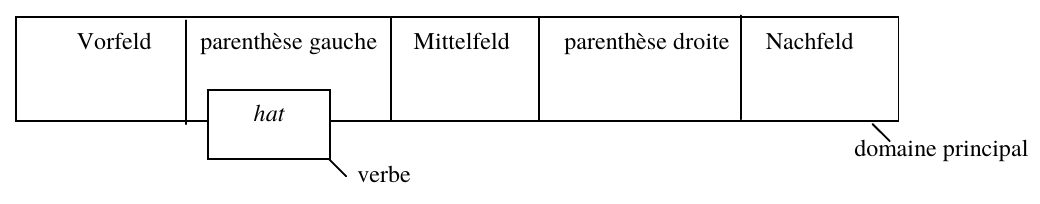
\includegraphics[width=\textwidth]{figures/vol1syntaxe2-img032.png}
   \begin{figure}[H]
      \begin{tabular}{|c|c|c|c|c|}
      \hline
      \multicolumn{5}{|c|}{\cellcolor{lsDOIGray}Domaine principal}\\
      \hline
      & {\cellcolor{lsDOIGray}parenthèse} &  & {parenthèse} & \\
       Vorfeld        & {\cellcolor{lsDOIGray}gauche}     &     Mittelfeld       &  droite      & Nachfeld \\
      \hline
      \end{tabular}
    \caption{Gabarit topologique du domaine principal de l'allemand\label{fig:gabarit-allemand}}
    \end{figure}

    Le verbe principal de la phrase, c’est-à-dire le verbe qui porte le mode indicatif, se place en 2\textsuperscript{e} position, appelée \hi{parenthèse gauche}, après l’unique constituant occupant le \hi{champ initial} ou \hi{Vorfeld} ‘pré-champ’. Les dépendants verbaux vont généralement dans la \hi{parenthèse droite}. La parenthèse gauche entoure avec la parenthèse droite, le \hi{champ du milieu} ou \hi{Mittelfeld}. Un \hi{champ final} ou \hi{Nachfeld} suit la parenthèse droite. Les \hi{champs} dits \hi{majeurs} -- Vorfeld, Mittelfeld et Nachfeld -- accueillent les différents syntagmes nominaux ou adverbiaux. 
    
    Considérons la phrase \REF{ex:leider} et son arbre de dépendance, donné dans la figure \ref{fig:leider}.
    
    \ea\label{ex:leider}
    \gll Leider hat Peter {mal wieder} in seiner Nase zu popeln gewagt   vor der ganzen Familie.\\
         Hélas   a   Peter   {une fois de plus}   dans son nez   de creuser osé   devant toute la famille\\
    \glt ‘Peter a malheureusement osé à nouveau se crotter le nez devant toute la famille.’
    \z
    
    \begin{figure}[H]
      \caption{Arbre de dépendance de \REF{ex:leider}\label{fig:leider}}
    \begin{forest} for tree={font=\itshape}
      [hat
        [leider]
        [gewagt
            [mal wieder]
            [zu popeln 
                [in seiner Nase]
                [vor der ganzen Familie]
            ]
        ]
      ]
    \end{forest}
   \end{figure}
   
    La racine de l'arbre de \REF{ex:leider}, l'auxiliare \textit{hat} `a' va dans la parenthèse gauche, tandis que le participe \textit{gewagt} 'osé' va dans la parenthèse droite, où il entraîne avec lui le verbe infinitif \textit{zu popeln} `de creuser', qui se place devant lui. Les verbes de la parenthèse droite ne peuvent pas accueillir leur dépendants nominaux et adverbiaux, qui vont donc s'émanciper et se placer dans le domaine principal. Un des constituants doit occuper le Vorfeld : ici c'est \textit{leider} qui occupe cette place, mais n'importe quel autre constituant aurait pu prendre la place.
    Le constituant \textit{vor der ganzen Familie} ‘devant toute la famille’ peut aller dans le Nachfeld, car il est assez lourd (et un placement dans le Mittelfeld séparerait trop les deux parenthèses). Des constituants légers comme \textit{mal wieder} ou \textit{Peter} préfèrent rester dans le Mittelfeld.

    Les propositions subordonnées, complétives et relatives, ont une structure réduite, sans Vorfeld, et l’élément qui introduit la proposition, le complémenteur ou le pronom relatif, occupe la parenthèse gauche. 

    \ea\label{ex:glaube}
    \gll  Ich glaube,   {\ob} dass Peter {mal wieder} in seiner Nase zu {popeln\textsubscript{3}} {gewagt\textsubscript{2}} {hat\textsubscript{1}}   {\cb}.\\
    Je crois   [ que  Peter {une fois de plus} dans son nez   de creuser  osé        a   ]\\
    \glt ‘Je crois que Peter a osé se crotter le nez à nouveau.’
    \z
    
    Le placement des verbes dans la parenthèse droite est assez contraint et peut aussi être décrit par une structure topologique, l’amas verbal. Il est composé de trois champs : le \hi{champ supérieur} ou \hi{Oberfeld}, le champ tête et le \hi{champ inférieur} ou \hi{Unterfeld} (voir la figure \ref{fig:topo-amas-allemand}). Le placement le plus courant est celui illustré en \REF{ex:glaube}, où chaque verbe subordonné se place à gauche de son gouverneur, c'est-à-dire dans le champ Oberfeld.

    \begin{figure}[H]
    \def\arraystretch{1.5}
    \setlength{\tabcolsep}{4ex}
    \begin{tabular}{|c|c|c|}
    \hline
    \multicolumn{3}{|c|}{\cellcolor{lsDOIGray}Amas verbal}\\
    \hline
    Oberfeld & \cellcolor{lsDOIGray}champ tête & Unterfeld\\
    \hline
    \end{tabular}
    \caption{Gabarit topologique de l'amas verbal en l'allemand\label{fig:topo-amas-allemand}}
    \end{figure}
    
    Sans rentrer dans tous les détails de l’amas verbal, remarquons que pour les dépendants de certains verbes, en particulier les modaux, l’Unterfeld est préférable à l’Oberfeld :

    \ea\label{ex:konnen}
    \ea[\textsuperscript{?}]{
    \gll Ich glaube,  {\ob} dass Peter {mal wieder} in seiner Nase {popeln\textsubscript{3}} {gekonnt\textsubscript{2} } {hat\textsubscript{1}}   {\cb}.\\
        Je crois  [ que   Peter {une fois de plus} dans son nez   creuser  pu           a   ]\\}
    \ex[]{
    \gll Ich glaube,  {\ob} dass Peter {mal wieder} in seiner Nase {hat\textsubscript{1}} {popeln\textsubscript{3}} {können\textsubscript{2}}   {\cb}.\\
    Je crois   [ que   Peter {une fois de plus} dans son nez  a     creuser  pu   ]\\
    \glt  ‘Je crois que Peter a pu se crotter le nez à nouveau.’}
    \z
    \z

    Dans l’exemple (\ref{ex:konnen}a), on observe l’ordre standard dans la parenthèse droite : l’infinitif \textit{popeln} ‘creuser’ se place dans l’Oberfeld du participe \textit{gekonnt} ‘pu’, lui-même placé dans l’Oberfeld de l’auxiliaire \textit{hat} ‘a’. On préfère en fait b, où un «~ersatz~» d’infinitif (all. \textit{Ersatzinfinitiv}), \textit{können} ‘pouvoir’, est réalisé au lieu du participe et où celui-ci est placé dans l’Unterfeld de l’auxiliaire, tandis que \textit{popeln} ‘creuser’ se place à nouveau dans l’Oberfeld de son gouverneur. Cette construction est appelée l’\textit{Oberfeldumstellung} ‘conversion du champ supérieur’. Pour certains locuteurs de l’allemand, le verbe \textit{popeln} peut se placer dans l’Oberfeld de l’auxiliaire, non occupé par le dépendant direct de l’auxiliare. Cette nouvelle construction est appelée le \textit{Zwischenstellung} ‘positionnement intermédiaire’ avec l’auxilaire entre les deux verbes à l’infinitif :

    \begin{exe}
    \exr{ex:konnen}
    \begin{xlist}
    \exi{c.} \gll Ich glaube,  {\ob} dass Peter {mal wieder} in seiner Nase  {popeln\textsubscript{3}} {hat\textsubscript{1}} {können\textsubscript{2}} {\cb}.\\
    Je crois   {\ob} que   Peter {une fois de plus} dans son nez  creuser  a     pu {\cb}\\
    \glt ‘Je crois que Peter a pu se crotter le nez {une fois de plus}.’
    \end{xlist}
    \end{exe}
}
\loupe[sec:3.5.37]{L’anglais comme langue de référence}{%
    Peu d’approches théoriques distinguent, comme nous le faisons, la structure syntaxique de la structure topologique. Nous pensons que la non-prise en compte de la topologie doit beaucoup au fait que l’anglais sert de langue de communication dans le monde scientifique et donc de langue de référence de très nombreux travaux en linguistique. Or l’anglais est, du point de vue typologique (c’est-à-dire lorsqu’on prend en compte la diversité des langues), une langue particulièrement «~exotique~». En effet, l’anglais a un ordre des mots singulièrement rigide, avec non seulement une position fixe du sujet devant le verbe, mais aussi l’obligation de placer l’objet direct avant les autres compléments. Cette particularité permet de postuler une sorte de groupe verbal (voir l’\encadref{sec:3.4.20} sur \textit{Le groupe verbal}) au niveau topologique en anglais. Par ailleurs, le fait que la structure syntaxique et la structure topologique soient si fortement liées peut amener à les identifier et donc à considérer aussi un constituant syntaxique VP (\textit{verb phrase}) au niveau syntaxique, comme le font les générativistes.

    Cela va plus loin encore, car les mêmes générativistes considèrent que toutes les langues devraient avoir un VP. Les langues qui autorisent le placement du sujet entre le V et l’objet, contredisant de fait l’existence d’un VP, sont alors dites \hi{non-configurationnelles}. Certains linguistes, dont Chomsky, considèrent qu’il y a bien un VP sous-jacent, mais que les syntaxèmes sont systématiquement déplacés en surface (voir l’\encadref{sec:3.2.6} sur \textit{Linéarisation et mouvement}). C’est une analyse que nous rejetons totalement.
}
\chevalier[sec:3.5.38]{Historique de la description topologique}{%
    Nous avons déjà mentionné à deux reprises la contribution de Gabriel \citet{girard1747vrais} à la modélisation de l’ordre des mots. Son ouvrage contient une dizaine de \hi{règles de précédence linéaire} remarquablement formalisées. Par exemple :

    \begin{quote}
    «~Première Règle. – Dans la forme expositive, le Subjectif marche ordinairement devant l’Attributif : celui-ci y précède à son tour l’Objectif et le Terminatif, lorsqu’ils sont énoncés par des expressions formelles et non simplement désignés par des pronoms personnels ou relatifs.~»
    \end{quote}

    Cette règle indique que, dans la phrase déclarative (= expositive), le sujet (= Subjectif) se place devant le prédicat verbal (= Attributif), qui lui-même précède l’objet direct (= Objectif) et l’objet indirect (= Terminatif), à moins que ceux-ci ne soient des pronoms personnels ou relatifs. Les règles suivantes de Girard indiquent que le sujet se place après le verbe dans les propositions en incise (Règle II), que le sujet peut se placer après le verbe en l’absence d’un objet direct ou quand celui-ci est un pronom (Règle III), etc.

    Le modèle topologique, avec ses gabarits de places fixes, s’est développé au siècle suivant en Allemagne. Simon \citet{herling1821uber} propose la première théorie globale sur la structure hiérarchique des phrases complexes de l’allemand basée sur des gabarits de places fixes. Oskar \citet{erdmann1886grundzuge} poursuit le travail de Herling en énumérant les types d’éléments que ces places peuvent contenir, donnant ce que \citet{Höhle1986} propose d’appeler le système de Herling-Erdmann et qu’on appelle plus souvent aujourd’hui la théorie des champs topologiques. Le terme \textit{Feld} ‘champ’ pour désigner ces places dans la phrase apparaît pour la première fois chez Erich \citet{drach1937grundgedanken} dans un livre intitulé~\textit{Grundgedanken der Deutschen Satzlehre} ‘Idées fondamentales de la phrase allemande’ destiné aux enseignants de l’allemand comme langue maternelle et langue étrangère. Le livre de Drach prône, avec une teinte légèrement nationalisante propre à l'époque, une émancipation de la grammaire allemande, qui était jusqu’à là sous une influence latine forte, en faveur d’une «~construction d’une présentation et d’un système de règles basé sur la nature de la langue allemande~». Gunnar \citet{bech1955studien} a adapté par la suite la terminologie de Drach pour décrire la structure interne du complexe verbal.

    Le modèle topologique a été appliqué par Povl \citet{skaarup1975premieres} à la description de l’ordre des mots en ancien français, montrant l’influence des langues germaniques sur l’émergence du français. \citet{gerdes2006amas} proposent le modèle topologique pour le français présenté dans ce chapitre, qui s’appuie notamment sur les travaux sur la macrosyntaxe de Claire \citet{blanche-benveniste1990francais}. Le modèle topologique a aussi été appliqué à des langues clairement non germaniques, comme dans la description par \citet{DonohueSag1999} du warlpiri, une langue aborigène d’Australie à ordre très libre.

    La question de l’ordre des mots a été peu traitée dans les premières grammaires formelles. Dans les grammaires de constituants, l’ordre linéaire est intégré à la structure syntaxique et toute variation de l’ordre des mots suppose un changement de structure syntaxique (voir l’\encadref{sec:3.2.7} \textit{De la non-séparation des ordres au mouvement}). Il faudra attendre le début des années 1980 pour que soient proposées des grammaires de constituants où les \hi{règles de précédence linéaire} sont séparées des règles de sous-catégorisation, notamment avec le modèle GPSG (\textit{Generalized Phrase Structure Grammar}, \citealt{gazdar1985generalized}), qui donnera ensuite HPSG (\textit{Head-driven Phrase Structure Grammar}, \citealt{PollardSag1987}). Le modèle topologique de l’allemand sera formalisé pour la première fois par Andreas \citet{kathol1995linearization-based} dans le cadre de HPSG.

    Dans le cadre des grammaires de dépendance, \citet{melcuk1987surface} proposent une liste très complète des constructions de l’anglais et des règles de précédence linéaire qui vont avec. Le modèle topologique sera formalisé en grammaire de dépendance simultanément par \citet{duchier2001topological} et \citet{gerdes2001word} (voir la formalisation proposée dans l’\encadref{sec:3.5.33} sur la \textit{Grammaire topologique formelle}).
}
\exercices{%\label{sec:3.5.39}
    \exercice{1} 
    \begin{enumerate}[label=\alph*.]
    \item Qu’est-ce que la topologie ?
    \item À quel endroit du modèle linguistique le modèle topologique intervient-il dans un modèle stratificationnel comme la théorie Sens-Texte (voir la \sectref{sec:1.3.8} \textit{Modularité et stratification} et l'\encadref{sec:1.3.9} \textit{La Théorie Sens-Texte}) ?
    \item Pourquoi rejetons-nous la notion d’ordre de base ?
    \end{enumerate}

    \exercice{2} (Ordre préfixé et postfixé.)
    \begin{enumerate}[label=\alph*.]
    \item On considère l’expression préfixée × 3 + × 12 5 7. Donner l’arbre de dépendance correspondant et en déduire une expression infixée et postfixée.

    \item On considère l’expression postfixée 1 5 ${\surd}$ + 2 /. Sachant que ${\surd}$ (racine carrée) est un opérateur unaire (c’est-à-dire d’arité 1), donner l’arbre de dépendance correspondant à cette expression. En déduire l’écriture traditionnelle de ce nombre (qui n’est autre que le nombre d’or).
    \end{enumerate}
    \exercice{3} (Projectivité.) Construire la structure de dépendance de la phrase suivante et vérifier qu’elle est non projective :

    \begin{exe} \exi{} À \textit{cette heure-là, je pense qu’il est déjà parti.} \end{exe}

    \exercice{4} (Théorie des graphes.) Le graphe K\textsubscript{4} n’est pas planaire extérieur (voir l'\encadref{sec:3.5.15} sur \textit{Projectivité et planarité}). Montrer qu’il est néanmoins planaire et que donc tous les graphes de 4 nœuds ou moins sont planaires. Chercher les graphes non-planaires les plus simples à 5 et à 6 nœuds.

    \exercice{5} (Topologie du groupe substantival en français.) On s’intéresse plus particulièrement au placement des déterminants et des numéraux en français. Comment rendre compte des données suivantes dans un modèle topologique ?

    \begin{exe}
    \sn
    \begin{xlista}
    \ex[]{\itshape les/mes/ces/deux/quelques/des/plusieurs amis sont venus}
    \ex[]{\itshape les/mes/ces deux/quelques amis sont venus}
    \ex[*]{\itshape les mes/ces/des/plusieurs amis sont venus}
    \ex[*]{\itshape amis sont venus}
    \end{xlista}
    \end{exe}

    \exercice{6} (Interrogation en français.) On observe un contraste entre le fonctionnement des interrogatifs \textit{à qui} et \textit{que~}:
    
    \begin{exe}
    \sn
    \begin{xlista}
    \ex[]{\itshape À qui parle-t-elle ?}
    \ex[]{\itshape À qui Marie parle-t-elle ?}
    \ex[]{\itshape Que dit-elle ?}
    \ex[*]{\itshape Que Marie dit-elle ?}
    \end{xlista}
    \end{exe}
    Comment expliquer cette différence de comportement dans le cadre d’un modèle topologique ?

    \exercice{7} (Topologie de l’anglais.) L’anglais possède une classe de verbes que l’on appelle les \terme{modaux} qui comprend les auxiliaires \textsc{be} ‘être’ et \textsc{have} ‘avoir’ et quelques verbes à valeur modale, comme \textsc{can} ‘pouvoir’, \textsc{must} ‘devoir’, \textsc{will} (auxiliaire du futur) ou \textsc{would} (auxiliaire du conditionnel), qui ont la particularité d’être invariables, ainsi que la proforme \textsc{do} ‘faire’. Ces verbes ont également des propriétés distributionnelles qui les distinguent des autres verbes. Premièrement, les adverbes se placent de préférence après les modaux et avant les verbes ordinaires :
    
    \begin{exe}
    \exi{(i)}
    \judgewidth{\textsuperscript{??}}
    \begin{xlista}
    \ex[]{\textit{Mary often calls Peter.}     ‘Marie appelle souvent Pierre.’}
    \ex[\textsuperscript{??}]{\textit{Mary calls often Peter.}}
    \ex[]{\textit{Mary would often call Peter.}   ‘Marie appellerait souvent Pierre.’}
    \ex[\textsuperscript{??}]{\textit{Mary often would call Peter.}}
    \end{xlista}
    \end{exe}
    Deuxièmement, dans les interrogatives, le sujet se place entre le modal et le verbe, et en cas d’absence de modal, \textsc{do} est introduit :
    
    \begin{exe}
    \exi{(ii)}
    \begin{xlista}
    \ex[]{\textit{Would Mary call Peter?}     ‘Marie appellerait-elle Pierre ?’}
    \ex[*]{\itshape Calls Mary Peter?}
    \ex[]{\textit{Does Mary call Peter?}     ‘Marie appelle-t-elle Pierre ?’}
    \end{xlista}
    \end{exe}
    La position initiale peut aussi être occupée par un pronom interrogatif :
    
    \begin{exe}
    \exi{(iii)}
    \begin{xlista}
    \ex[]{\textit{Why would Mary call Peter?}   ‘Pourquoi Marie appellerait-elle Pierre ?’}
    \ex[]{\textit{Who does Mary call?}     ‘Qui Marie appelle-t-elle ?’}
    \end{xlista}
    \end{exe}
    Troisièmement, la négation se place obligatoirement sur un modal et donc comme dans le cas de l’interrogation, \textsc{do} doit être introduit en l’absence d’un autre modal :
    
    \begin{exe}
    \exi{(iv)}
    \begin{xlista}
    \ex[]{\textit{Mary would not call Peter.}     ‘Marie n’appellerait pas Pierre.’}
    \ex[*]{\itshape Mary calls not Peter.}
    \ex[]{\textit{Mary does not call Peter.}    ‘Marie n’appelle pas Pierre.’}
    \end{xlista}
    \end{exe}
    Quatrièmement, le sujet peut être inversé dans certains cas :
    
    \begin{exe}
    \exi{(v)}
    \begin{xlista}
    \ex  \textit{Never does Mary call Peter.}   ‘Jamais Marie n’appelle Pierre.’
    \ex  \textit{Here are two nice people.}     ‘Ici sont deux chouettes personnes.’
    \end{xlista}
    \end{exe}
    Rappelons également que, en anglais, l’objet direct doit précéder tous les autres compléments. De quelle façon un modèle topologique de l’anglais peut-il rendre compte de ces propriétés ?

    \exercice{8} (Topologie de l’allemand.) Les exemples que nous avons présentés dans l’\encadref{sec:3.5.36} acceptent encore d’autres ordres, comme, par exemple :

    \begin{exe}
    \sn
    \gll In seiner Nase zu popeln hat Peter {mal wieder} gewagt.\\
         dans son nez  de creuser  a   Peter   {une fois de plus}   osé\\
    \glt   ‘Peter a à nouveau osé se crotter le nez.’
    \end{exe}
  Comment pouvez-vous intégrer cet exemple au modèle topologique de l’allemand ?

    \exercice{9} Ce que nous avons fait pour le français, l’allemand, le russe ou l’anglais peut être fait pour n’importe quelle langue a priori. Nous avons déjà écrit des modèles topologiques pour l’arabe, le chinois ou le wolof. Vous pouvez essayer d’écrire un fragment de modèle topologique pour la langue de votre choix et nous l’envoyer.
}
\lecturesadditionnelles{% \label{sec:3.5.40}
    Comme nous l’avons déjà mentionné au \chapref{sec:3.3}, on peut consulter en ligne la plupart des ouvrages anciens. On trouvera facilement \citet{buffier1709grammaire}, \citet{girard1747vrais}, \citet{gaultier1817atlas}, \citet{weil1844de}, ainsi que les articles de Beauzée et Dumarsais dans l’\textit{Encyclopédie} de Diderot et D’Alembert (voir le \chapref{sec:3.3}).

    Les premiers travaux sur le modèle topologique sont en allemand : \citet{erdmann1886grundzuge}, \citet{drach1937grundgedanken}, \citet{bech1955studien}. Pour des travaux plus récents sur l’ordre des mots, nous avons mentionné \citet{gazdar1985generalized}, \citet{pollard1994head-driven}, \citet{melcuk1987surface}, \citet{kathol1995linearization-based}, ainsi que les articles de \citet{bresnan2007predicting}, \citet{duchier2001topological} et \citet{gerdes2001word,gerdes2006amas}. Sur la structure communicative et son rôle dans l’ordre des mots, nous renvoyons à \citet{lambrecht1996information} et \citet{melcuk2001communicative}.

    Pour les travaux typologiques sur l’ordre des mots, on consultera l’article original de \citet{greenberg1963universals} et l’étude et le travail très complet de \citet{dryer1992greenbergian}, ainsi que les cartes et les différents articles consacrés à l’ordre des mots sur le site \url{wals.info}, une base de données typologique où sont répertoriés 192 traits pour plus de 2500 langues !

    \FurtherReading{3-5}
}
\corrections{%\label{sec:3.5.41}
    \corrigé{1}
    \begin{enumerate}[label=\alph*.]
    \item La topologie est l’étude du placement des unités syntaxiques, c’est-à-dire l’étude de l’ordre des mots, mais aussi des syntaxèmes à l’intérieur des mots.

    \item Le modèle linguistique décrit la correspondance entre le sens et le texte. Le modèle topologique décrit la linéarisation, c’est-à-dire la correspondance entre la structure syntaxique (non ordonnée) et la chaîne linéaire. Ou dans sa version plus élaborée entre une structure de dépendance syntaxique et un arbre de constituants topologiques.

    \item Certaines langues ont un ordre dominant, comme l’ordre SVO en français. Néanmoins considérer un ordre de base revient à considérer que tous les autres ordres sont obtenus par des transformations de l’ordre base. Cela revient à dire que lorsque le sujet est après le verbe en français, celui-ci a été inversé. Même s’il peut nous arriver de conserver la terminologie et de parler de «~sujet inversé~», nous ne considérons pas qu’il y a eu une inversion. Nous considérons que le sujet a été placé directement dans cette position.
    \end{enumerate}
    \corrigé{2} 
    \begin{enumerate}[label=\alph*.]
    \item Le premier symbole, $\times$, est la racine de l’arbre. Son premier dépendant est 3. Le symbole suivant, +, est la racine du deuxième dépendant, et ainsi de suite. La formule est donc $3 \times \left((12\times5) + 7\right)$ sous forme infixée et 3 12 5 $\times$ 7 + $\times$ sous forme postfixée.

    \item La formule est (1 + $\sqrt{5}$) / 2 sous forme infixée et / + 1 $\surd$ 5 2 sous forme préfixée.
    \end{enumerate}

    \corrigé{3} Le syntagme \textit{à cette heure-là} dépend de \textit{parti} et couvre donc la racine de l’arbre \textit{pense}.

    \corrigé{4} Le graphe K\textsubscript{4} est planaire : il suffit de prendre une des diagonales et de la faire passer par l’extérieur du carré. C’est le plus complexe des graphes à 4 nœuds et donc tous les graphes à 4 nœuds ou moins sont planaires. Le plus petit graphe non planaire à 5 nœuds est K\textsubscript{5}, le graphe complet à 5 nœuds. Le plus petit graphe non planaire à 6 nœuds est K\textsubscript{3,3}, le graphe où 3 nœuds sont liés aux 3 autres. On vérifiera que, si on retire un seul de leurs liens, ces graphes deviennent planaires.

    \begin{center}
    \begin{minipage}[c]{.5\linewidth}\centering
      \begin{tikzpicture}
      \begin{scope}[local bounding box=graph,every node/.style={CircleNode}]
        \graph [clockwise, empty nodes] { subgraph K_n [n=5] };
      \end{scope}
        \node[below=1pt of graph] {K\textsubscript{5}};
      \end{tikzpicture}
    \end{minipage}\begin{minipage}[c]{.5\linewidth}\centering
      \begin{tikzpicture}
      \begin{scope}[local bounding box=graph,every node/.style={CircleNode}]
        \graph [empty nodes, branch right, grow down] { subgraph K_nm [n=3, m=3] };
      \end{scope}
        \node[below=1pt of graph] {K\textsubscript{3, 3}};
      \end{tikzpicture}
    \end{minipage}
    \end{center}

    Le mathématicien polonais Kazimierz Kuratowski a établi en 1930 la caractérisation suivante des graphes planaires : un graphe est \hi{planaire} si et seulement s’il ne peut être réduit ni à K\textsubscript{5}, ni à K\textsubscript{3,3}.

    On pourra consulter les pages de la wikipédia sur les graphes planaires et planaires extérieurs.

    \corrigé{5} On observe trois paradigmes de «~déterminants~» : 1) \textit{les, mes, ces~}; 2) \textit{des, plusieurs~}; 3) \textit{deux, quelques}. Les éléments de types 1 et 3 peuvent cooccurrer, tandis que ceux de types 2 excluent les autres. Les noms communs doivent obligatoirement être accompagnés d’au moins un éléments d’un de ces trois types. Les éléments de type 1 sont les déterminants définis, ceux de type 2 les déterminants indéfinis. Quant à ceux de type 3, ce sont des quasi-déterminants, puisqu’ils peuvent se placer entre un déterminant défini et le nom et qu’ils n’ont pas de valeur intrinsèquement définie ou indéfinie, mais ils prennent une valeur indéfinie en l’absence d’un déterminant défini. On peut modéliser cette distribution en considérant deux champs topologiques : un pour les déterminant définis, suivi d’un pour les quasi-déterminants, avec la condition qu’un des deux champs au moins doit être occupé. Les déterminants indéfinis occuperaient quant à eux les deux champs en même temps. (Ou ce qui revient au même, ils occupent le champ des quasi-déterminants, mais excluent, pour des raisons sémantiques, la cooccurrence avec un déterminant défini.)

    \corrigé{6} Les pronoms interrogatifs se placent au début du domaine microsyntaxique, devant le sujet (dans \textit{Marie, à qui parle-t-elle} ?, \textit{Marie} est détaché et n’occupe plus la position sujet). Le pronom interrogatif \textit{que} est la forme faible du pronom \textit{quoi} (comme \textit{me} avec \textit{moi}). C’est un clitique qui doit obligatoirement être dans l’amas verbal (comme \textit{me}). Autrement dit, le pronom interrogatif \textit{que} doit à la fois être en tête du domaine microsyntaxique et dans l’amas verbal, ce qui écrase tout ce qui se trouve entre les deux et en particulier le champ initial qu’occuperait le sujet.

    \corrigé{7} Les modaux de l’anglais occupent un champ topologique différent de celui des verbes. Le domaine microsyntaxique de la phrase déclarative est donné dans la figure \ref{fig:domaine-anglais}.
    
    \begin{figure}[H]
      \caption{Domaine verbal microsyntaxique de l'anglais\label{fig:domaine-anglais}}
      \begin{tabular}{|c|c|c|c|c|c|}
        \hline
        \multicolumn{6}{|c|}{\cellcolor{lsDOIGray}Domaine microsyntaxique}\\
        \hline
        ch\_initial & ch\_modal & ch\_adv & ch\_verbal & ch\_objet & ch\_compl\\\hline
      \end{tabular}    
    \end{figure}

    Le sujet va dans le champ initial, sauf quand celui-ci est occupé par un pronom interrogatif, une négation ou un locatif, ou quand il reste vide dans une interrogative totale. Le champ modal peut rester vide quand le sujet occupe le champ initial et qu’il n’y a pas la négation \textit{not} dans le champ adverbial. Lorsque le champ initial est occupé par un autre élément, le sujet va dans le champ adverbial. Dans les interrogatives le sujet ne peut pas occuper le champ initial, qui peut rester vide en l'absence d'un pronom interrogatif. Le champ modal doit obligatoirement être occupé si le sujet n'est pas dans le champ initial.

    \corrigé{8} Cet exemple montre qu’un constituant à tête verbale, comme \textit{in seiner Nase zu popeln} ‘de se crotter le nez’, peut également venir se placer dans le Vorfeld. Nous avons vu un cas similaire dans l'exemple (\ref{ex:Nase-participe}a), où un verbe au participe passé est placé dans le Vorfeld. Il suffit d'indiquer, dans la règle de correspondance de placement dans le Vorfeld, quelles sont la catégories syntaxiques qui sont éligibles.
    Il n’est pas nécessaire d’aménager davantage le modèle.
}
